\documentclass[12pt,twoside]{reedthesis}

\usepackage{graphicx,latexsym}
\usepackage{amssymb,amsthm}
\usepackage{longtable,booktabs,setspace}
\usepackage[hyphens]{url}
\usepackage{rotating}
\usepackage{outlines}
\usepackage{enumitem} % custom labels

% font stuff
\usepackage{bbm, stmaryrd}
\usepackage{luatexja} % for memes

\usepackage{amsmath}
\usepackage{mathtools} % paired delimeters
\usepackage{braket}
\usepackage{epigraph} % funny quotes
\usepackage{tikz-cd} % diagrams
\usepackage{circuitikz} % circuit diagrams
\usepackage{emoji}
\usepackage{quiver} % fancy arrows

\usepackage{mathpartir} % inference rules

\usepackage[
backend=biber,
style=alphabetic,
citestyle=alphabetic
]{biblatex} % better citation style
\addbibresource{thesis.bib}

\usepackage{hyperref}

\hypersetup{
  colorlinks,
  allcolors=black,
  hidelinks,
}

\theoremstyle{definition}
\newtheorem{theorem}{Theorem}[section]
\newtheorem{definition}[theorem]{Definition}
\newtheorem{example}[theorem]{Example}
\newtheorem{joke}[theorem]{Joke}
\newtheorem{notation}[theorem]{Notation}
\newtheorem{remark}[theorem]{Remark}
\newtheorem{lemma}[theorem]{Lemma}
\newtheorem{Recall}[theorem]{recall}
\newtheorem{corollary}[theorem]{Corollary}

% \newcommand{\sslash}{\mathbin{/\mkern-6mu/}}
\newenvironment{sketch}{\textit{Sketch.}  }{\hfill$\sslash$}

%%% From user4686 on the TeX stackexchange. Thank you!
%%% https://tex.stackexchange.com/a/289552
\newcommand*\autoop{\left(}
\newcommand*\autocp{\right)}
\newcommand*\autoob{\left[}
\newcommand*\autocb{\right]}
\DeclareRobustCommand*\{{\ifmmode \left\lbrace \else \textbraceleft \fi }
\DeclareRobustCommand*\}{\ifmmode \right\rbrace \else \textbraceright \fi }
\AtBeginDocument {%
   \mathcode`( 32768
   \mathcode`) 32768
   \mathcode`[ 32768
   \mathcode`] 32768
   \begingroup
       \lccode`\~`(
       \lowercase{%
   \endgroup
       \let~\autoop
   }\begingroup
       \lccode`\~`)
       \lowercase{%
   \endgroup
       \let~\autocp
   }\begingroup
       \lccode`\~`[
       \lowercase{%
   \endgroup
       \let~\autoob
   }\begingroup
       \lccode`\~`]
       \lowercase{%
   \endgroup
       \let~\autocb
   }}

\delimiterfactor 1001

\makeatletter
% for amsmath "compatibility" (not sophisticated)
% \usepackage{amsmath}
\AtBeginDocument {%
          \def\resetMathstrut@{%
           \setbox\z@\hbox{\the\textfont\symoperators\char40}%
           \ht\Mathstrutbox@\ht\z@ \dp\Mathstrutbox@\dp\z@}%
}%
\makeatother

% thanks to this guy https://tex.stackexchange.com/a/101138
\usepackage{scalerel}
\usepackage{stackengine,wasysym}

\newcommand\reallywidetilde[1]{\ThisStyle{%
  \setbox0=\hbox{$\SavedStyle#1$}%
  \stackengine{-.1\LMpt}{$\SavedStyle#1$}{%
    \stretchto{\scaleto{\SavedStyle\mkern.2mu\AC}{.5150\wd0}}{.6\ht0}%
  }{O}{c}{F}{T}{S}%
}}

\newcommand{\term}{\emph} % TODO: make a tool to grab all the emph's from my
                          % document and optionally add them to the glossary
\newcommand{\id}{\textrm{id}}

\def\bitcoin{%
  \leavevmode
  \vtop{\offinterlineskip %\bfseries
    \setbox0=\hbox{B}%
    \setbox2=\hbox to\wd0{\hfil\hskip-.03em
    \vrule height .3ex width .15ex\hskip .08em
    \vrule height .3ex width .15ex\hfil}
    \vbox{\copy2\box0}\box2}}


\hyphenation{pre-sheaves}

\DeclarePairedDelimiter\ceil{\lceil}{\rceil}

% Comment out the natbib line above and uncomment the following two lines to use the new 
% biblatex-chicago style, for Chicago A. Also make some changes at the end where the 
% bibliography is included. 
% \usepackage{biblatex-chicago}
% \bibliography{thesis}

% \usepackage{times} % other fonts are available like times, bookman, charter, palatino

\title{The Way of Glue\\ An Invitation to the Categorical Semantics of Lambda
  Calculi} \author{Jay Kruer}
% The month and year that you submit your FINAL draft TO THE LIBRARY (May or December)
\date{December 2021}
% \division{Mathematics and Natural Sciences}
\advisor{Ang\'elica Osorno}
\altadvisor{James (Jim) Fix}

\department{Mathematics and Computer Science}
% if you're writing a thesis in an interdisciplinary major,
% uncomment the line below and change the text as appropriate.
% check the Senior Handbook if unsure.
\thedivisionof{The Established Interdisciplinary Committee for\\ Mathematics and Computer Science}
% if you want the approval page to say "Approved for the Committee",
% uncomment the next line
% \approvedforthe{Committee}

\setlength{\parskip}{0pt}

\begin{document}
\maketitle
\frontmatter % this stuff will be roman-numbered
\pagestyle{empty} % this removes page numbers from the frontmatter

% Acknowledgements (Acceptable American spelling) are optional So are
% Acknowledgments (proper English spelling)
\chapter*{Acknowledgements}
It's not often in life one gets a chance to thank the many people who have
helped him on his way, so I've spent the last few months slowly accumulating a
list of people I'd like to thank whether for their direct impact in making this
thesis possible or just for having had an outsized impact on my life at one
point or another. I can only start by thanking my advisors Ang\'elica and Jim
for their part in making my thesis year one of my favorite's in my time at Reed
and for making this thesis possible. I am first of all indebted to Ang\'elica's
spooky ability to instantly grasp at understanding even in an area relatively
unknown to her. Without her hints at how to tackle an opaque construction every
now and then, I think I'd probably be still fumbling around with the basics. Jim
has had an outsized influence on the direction my intellectual life has taken.
Jim's intro CS course taught partially in Standard ML was my first real exposure
to mathematically structure programming and opened up to me a world that had
until then had seemed inaccessible. Jim has also served as a great mentor in
matters of personal taste and style (his course webpages are always out of this
world cool.) I'll really miss our wacky math-cs crossover meetings, you two!

The students and faculty in the math department have made the last few years a
profoundly enriching experience. Albyn Jones and Irena Swanson, who taught my
intro courses freshman year, are singled out for special thanks. I was not by
any stretch a likely math major by the time I came to Reed. Having been brought
from complete ignorance to a great appreciation for mathematics under Albyn and
Irena's careful guidance was a great privilege and one I'll remember fondly all
my life! I am also grateful to Kyle Ormsby for always being an absolute chiller,
encouraging me in some early ambitions, and for giving me a taste of category
theory before I fled from his topology class.

Now the acknowledgements become less organized, but by no means less sincere!

None of this would have been possible without my Mom and Dad. Thanks so much!

Jaclyn, my love, thank you for being everything to me over the past (almost!)
two years and for your friendship for the last (almost) 4. You turned an ugly
quarantine into a beautiful one, and I can't wait to spend the rest of it (and
more!) with you.

Thank you to Uncle Jay for your constant encouragement for my interests in
computers. And to Grandma, Aunt Julie, Aunt Susie, and all of my extended family
for your continued support!

A few teachers have made a huge impact on my life. My high school Chinese
teacher 吳老師 (Rhoda Weston) is the most generous person I've ever met, in so
many ways, and just about changed my life. Thank you for making it possible for
me to go to Taiwan and for everything else! Thank you to my first grade teacher
Ms.\ King for being a fantastic example of living with kindness, to 柳老
師 (Hyong Rhew) for getting me to chill out a bit freshman year\footnote{Thanks
  also for comparing me to a metal waterbottle for some reason\dots never
  figured that one out.} and hours of fun studying Chinese, to Mrs.\ Leitsch for
stellar teaching and encouragement in 9th grade English, to Mr. Cool for good
times on the robotics team (even if you wouldn't let us switch from LabView),
and to my 4th (?) grade history teacher Mr.\ Raveli for teaching me that it's
better to know how and where to find the answers than to have them all committed
to memory.

More than anything, friends have made the last few years special:

Thanks to the hyperbolic crew---Francis Baer, Alec Forget, Usman Hafiz, Kiana
McBride, and Luke Doms---for helping to make Kyle's wild ride a dummy good time.

Thanks to the many friendbobs of pika: Joebob, Jit, Eli, Gabe and Ciara, Becca,
Andres, Nathan, Chloe. The time I spent with you all in Boston was and remains
precious to me beyond measure!

Thanks to Aaron Weiss for being a constant companion (even over discord) over
the last 3 years. I'm so glad we ended up labmates! Stay fresh, king.

The following people made my freshman year at Reed. Thank you to Holden and Max
for making WP117 home. Special thanks to Max for not holding against me my
having thrown a mug at him, and to Holden for never violating the NAP. Thanks to
Noah Koster for being one of my very first friends at Reed and for always
truckin'. You may not be the next Bill Gates, but you're a great guy. Thanks to
Nick Chaiyachakorn for always encouraging my stupid computer purchases, and for
just always being there for me. Thanks to Yuta, Shulav, Jake, and Aditya for
many fine hours of good lad time. Thanks to Carter Fife for ditching us all and
for being a massive weeb, to Dan Jeon for telling everyone about that time he
caught me practicing Naruto hand signs, to Mary Brady for showing me the best
song of the century (Freaky Friday by Lil Dicky ft. Chris Brown), and to Salma
Huque for being poggers.

The following people made my sophomore year much more tolerable. Thanks to
Genya, Tristan, and the rest of the crew for so many great nights in Polytopia.
Special thanks go to Young Kim for corrupting my soul. This thesis is in some
sense a tribute to you, because I know how much you love category theory. Thanks
also to Alice McKean for good times talkin' type theory.

Thank you to my beloved 1989 Toyota TownAce van which made the early pandemic an
absolute adventure. I'll miss you forever :'(

My deep thanks go to Amal Ahmed for taking me on and guiding my early studies of
programming language theory during my leave from Reed. I came to her with a lot
of enthusiasm to learn and not much else, and she gave me a wonderful
opportunity to make good on that enthusiasm. Without her guidance I would not be
writing a thesis like this today, and I'll always be indebted to the influence
she's had on my way of thinking about computing.

Thanks to Murali Vijayaraghavan for mentorship and patient instruction while I
was learning the ropes the ropes of CPU and hardware design. Thanks to Cody Roux
and Dan McArdle (then at Draper Lab) for early encouragement!

Thank you to Sara Rosenberger in the business office for having my back when the
office of financial aid left me to rot. This thesis couldn't have happened
without you!

Thanks to my sister Megan for her unrelenting support, especially over the last
few challenging years! and for her patience putting up with my various neuroses!
Thanks to my brother Ryan and my sister Kathleen for always being there.

Thank you to the composers of Breath of the Wild and to lofi girl for the
soundtrack.

I owe a huge debt to the great and generous people of the \TeX\ StackExchange
for \TeX macros used in the production of this document. Thank you to user4586
for their automatically-sized delimeters macro, to Steven B. Segletes for their
really wide tildes macro, and to user13907 for their stylized B symbol. Thank
you to the various people involved in the creation of the Lua \LaTeX\ system, in
whatever capacity. Free software development is often thankless work, and I hope
that recognizing it in this small way means something to the authors of these
tools.

Thank you to Steve Awodey for listening to me deliver a draft version of the
argument laid out in Chapter 3 and for helpful comments. Thanks to Carlo Angiuli
for answering a question about the category of renamings. Thank you to Ivan Di
Liberti for many fun and useful mentorship Zoom meetings throughout the last few
months!

I would like to give special thanks to Paul Taylor who wrote the book that made
this thesis possible. Paul's \emph{Practical Foundations of Mathematics} is one
of the great books of computing, in the same league as Knuth's \emph{Art of
  Computer Programming} in that it is not just a useful centralization of human
knowledge but that the presentation is painstakingly beautiful. On nearly all of
the early days spent on this project I learned from Paul's book a profound
perspective on programming or mathematics in general.

My thanks also go to Jon Erickson, author of \emph{Hacking: The Art of
  Exploitation} which got me started on this road so many years ago. What a long
and strange road to a thesis about huffing (strictly in the mathematical sense)
glue!

% The preface is optional
% To remove it, comment it out or delete it.
% \chapter*{Preface}


% I don't know what to put here, but this is certainly a funny quote that should
% find a home somewhere in the thesis.

\chapter*{Notation}
The face \( \mathfrak{Mathfrak}\) is used to denote presheaves, namely, objects
in the category \( {\catset}^{C^{\textrm{op}}}\) for any category \( C \).


% \chapter*{List of Abbreviations}
% \begin{table}[h]
%   \centering % You could remove this to move table to the left
%   \begin{tabular}{ll}
%     \textbf{TMA}  	&  Too Many Abbreviations
%   \end{tabular}
% \end{table}


\tableofcontents
% if you want a list of tables, optional
\listoftables
% if you want a list of figures, also optional
% \listoffigures

% The abstract is not required if you're writing a creative thesis (but aren't they all?)
% If your abstract is longer than a page, there may be a formatting issue.
\chapter*{Abstract}
Normalization by gluing is based.

% \chapter*{Dedication}


\mainmatter% here the regular arabic numbering starts
\pagestyle{fancyplain} % turns page numbering back on

\setlength{\headheight}{14.49998pt}
\overfullrule=1mm

% The \introduction command is provided as a convenience.
% if you want special chapter formatting, you'll probably want to avoid using it altogether

\chapter*{Introduction}
\epigraph{And further, by these, my son, be admonished: of making many books
  there is no end; and much study is a weariness of the flesh.}{Ecclesiastes
  12:12, KJV.}
\addcontentsline{toc}{chapter}{Introduction}
\chaptermark{Introduction}
\markboth{Introduction}{Introduction}
% The three lines above are to make sure that the headers are right, that the intro gets included in the table of contents, and that it doesn't get numbered 1 so that chapter one is 1.

% Double spacing: if you want to double space, or one and a half 
% space, uncomment one of the following lines. You can go back to 
% single spacing with the \singlespacing command.
% \onehalfspacing
% \doublespacing

Though we encounter many interesting objects and ideas along the way, this
thesis is primarily concerned with the \emph{open normalization} problem for the
simply typed lambda calculus. Some explaining is in order. First, we'll talk
about the simply typed lambda calculus. The reader might be familiar with the
\emph{untyped} lambda calculus. The lambda calculus is a formal system oriented
toward the study of functions and their \emph{applicative} behavior
\cite{barendregt_lambda_2012}. We define a notion of function abstraction which
allows us to select \emph{bound} variables from the variables appearing in some
mathematical phrase, as in \( \lambda x.\, x^{2}\). The fundamental operation of the
lambda calculus is \emph{application}, which is defined in terms of
\emph{substitution}. The application of a function \( f \) to an argument
\( a \) is denoted by juxtaposition as in \[ f a. \] A more concrete example of
application is \( \sin \pi \). Function application is a derived notion; what
application \emph{does} is defined in terms of \emph{substitution}. For phrases
(henceforth called \emph{terms}) $e$ and $e'$, we impose an equation
\[ (\lambda x.\, e) e' = [e' / x]^{*}e \] called the \( \beta \)-\emph{law}. When
writing \[ [s/x]^{*} p, \] we mean the term given by taking the term $p$ and
replacing with $s$ every occurrence of $x$ appearing within. Authors more
interested in the computational character of the \emph{lambda calculus} write
\[ (\lambda x.\, e) e' \rightarrow [e' / x]^{*}e\] so that \( \beta \) principle is instead
understood as a \emph{reduction rule} for an \emph{allowed transition} or
\emph{computation step}. For our purposes, we will mostly be working with
equations except in remarks meant to appeal to those readers who are
operationally inclined.

The famed Church-Turing thesis says that the lambda calculus and the Turing
machine, a more famous model of universal computation, are \emph{equivalent in
  computational power}. That is, any Turing machine can be simulated by the
lambda calculus and conversely any program written in the lambda calculus can be
simulated by some Turing machine. Consequently, just as the Turing machine is a
universal computer, the lambda calculus is a universal programming language.
That the lambda calculus is so powerful is exciting, but some consider working
with that full power unwieldy or even dangerous. Indeed, there are programs that
one can write down in the lambda calculus which get ``stuck'' before computing a
\emph{value}, meaning that there are lambda programs $p$ which reduce to a $p'$
which isn't a value but cannot be reduced to some $p''$.

The usual solution to this problem is to tie our own hands a bit, imposing a
regime of \emph{types} which allow us to statically rule out those program
states (i.e., stuck terms) that we don't want to happen. The simplest example of
such a regime is, appropriately, \emph{simple types}. The simply-typed lambda
calculus enriches the lambda calculus with some base types, say booleans and
natural numbers, along with derived types \( A \times B\) representing \emph{pairs of
  terms} of the types $A$ and $B$ along with \( A \Rightarrow B\) representing
\emph{functions} taking an $A$ and giving a $B$. For example, the type
\( \mathbbm{B} \times \mathbbm{N}\) is inhabited by pairs of a boolean and some
natural number. Along with this type structure comes \emph{rules} stipulating
how it may be used. We will not explain this story in depth in this thesis, but
we will soon see these rules in Chapter~\ref{chapter:stlc}. The desired result
indeed follows from this setup: lambda terms that follow the typing rules do not
get stuck when evaluated. This is one instance of the famed \emph{type safety}
properties of programming language theory. Another family of properties, namely
\emph{normalization} properties, follows from this type regime. It turns out
that any program in the lambda calculus will reduce to a value in a finite
number of evaluation steps. This property is called \emph{closed normalization}.
Borrowing the language of the theory of Turing machines, this means that
programs written in the simply typed lambda calculus always halt. In particular,
this means that the lambda calculus is \emph{not} Turing complete and can only
simulate deciding Turing machines. This can be a problem for some applications.
If you want, say, your web server to run indefinitely without bound; the simply
lambda calculus can't do that. You could, however, make your program loop until
the projected death of the sun and deploy a new version of your server shortly
thereafter. Having noted that there are some workarounds to the problems arising
from the terminating character of the simply typed lambda calculus, it is
interesting to note also that this very character is actually required for some
applications; for some purposes, non-terminating languages have no such cute
workarounds.

An \emph{interactive theorem prover} is a computer program that allows a
computer user to state theorems and input proofs\footnote{Individual systems
  vary in how manual the process of inputting proofs is.}, which are then
checked by the program. Many interactive proof systems, such as Coq or Agda, are
based on type\footnote{Here I am referring to type theory in the same sense as
  above for the simply typed lambda calculs. Only the type systems underlying
  modern proof assistants feature much more complicated type structure, which is
  precisely what enables them to express non-trivial mathematical statements and
  proofs. We will see a little more on this story below.} theory. Such proof
systems leverage a principle called the \emph{Curry-Howard isomorphism}, which
allows one to represent theorems as \emph{types} and proofs as \emph{programs}.
The advanced type theories of such systems allow one to state and prove the sort
of universally and existentially quantified propositions one often encounters in
mathematics. An \emph{absolutely critical} property for systems like this is
that the proof construction language (remember that this is analogous to a
programming language according to the Curry-Howard isomorphism) be terminating,
for the following reason. Suppose you have stated a proposition $P$. The
Curry-Howard isomorphism allows us to represent $P$ by a type $T_{P}$ such that
constructing a term (a program potentially with parameters) $t$ with type
$T_{P}$ amounts to proving the proposition $P$. Given any type, I can give you a
non-terminating program of that type. This is easiest to see by putting
unguarded termination in the language as a form of non-termination. The program
simply calls itself recursively forever, infinitely passing the buck but
ostensibly having the desired type. Let's check out an example in the Coq proof
assistant; we will be deriving a term of type False (the type which has no term
constructors, and hence really ought to be uninhabited.) You could perform this
same construction for any type you choose, even if it would be redundant now
that we have a False term (which gives us a term of any other type by trivial
case analysis). We first manually deactivate a Coq safety feature expressly
intended to rule out such definitions.

\begin{verbatim}
j@art-house-thinking-sand ~ % coqtop
Welcome to Coq 8.14.0

Coq < Unset Guard Checking.

Coq < Fixpoint falso (u : unit) : False := falso tt.
falso is defined
falso is recursively defined (guarded on 1st argument)
\end{verbatim}

If we reset \emph{guard checking}, which places restrictions on the allowed
forms of recursive definitions so that they are \emph{well-founded}, we find
that Coq refuses this definition.

\begin{verbatim}
Coq < Set Guard Checking.

Coq < Fixpoint falso (u : unit) : False := falso tt.
Toplevel input, characters 0-46:
> Fixpoint falso (u : unit) : False := falso tt.
> ^^^^^^^^^^^^^^^^^^^^^^^^^^^^^^^^^^^^^^^^^^^^^^
Error:
Recursive definition of falso is ill-formed.
In environment
falso : unit -> False
u : unit
Recursive call to falso has principal argument equal to
"tt" instead of a subterm of "u".
Recursive definition is: "fun _ : unit => falso tt".
\end{verbatim}

With this fact in mind, normalization proofs for the underlying proof language
are an essential requirement for a trustworthy interactive theorem proving
system; otherwise there is no guarantee that proofs of false theorems as above
are unavailable. It should be noted that non-termination is only one source of
inconsistency and that we should demand much more than termination of our
theorem proving systems.

Normalization theorems like these are typically proven using a technique called
\emph{the method of logical relations}\footnote{Normalization proofs actually
  only require the use of \emph{logical predicates}, which are the unary case of
  logical relations, but the general method is better known by the name
  \emph{logical relations}.} We will learn a bit more about logical relations in
the third chapter. The normalization theorem of interest to people concerned
with the safety of proof assistants are a little more challenging, and demand a
leap in technology to the method of \emph{Kripke logical relations}, also
detailed in Chapter~\ref{chapter:gluing}. The class of normalization theorems of
interest to implementors of proof assistants is called the problem of \emph{open
  normalization}, and is in fact the type of theorem we will work toward in this
thesis. Our \emph{open normalization} theorem will be stated somewhat
differently than the \emph{closed normalization} statement given above. Rather
than speaking directly about the behavior of terms undergoing reduction, we will
work with \emph{equivalence classes} of terms taken over an equality
\emph{generated by} the reduction rules of the lambda calculus. Our
normalization theorem will demand that we produce a \emph{function} from
ordinary open terms to normal forms which both preserves and reflects these
equivalence classes of terms. The reason that such a device is interesting to
implementors of proof assistants is that proof assistants are usually based on
\emph{dependent type systems}, in which the language of types allows for the
presence of general terms. Such advanced type systems are the ones alluded to
earlier in this introduction during our discussion of the Curry-Howard
isomorphism. The Curry-Howard isomorphism casts the task of proof verification
as the task of typechecking. Because dependent type theory allows for arbitrary
terms (and in particular \emph{programs}) inside of types, the task of
typechecking in this setting amounts to deciding the equality of the final
\emph{result} of arbitrary subterms (and, in particular, arbitrary
sub\emph{programs}). In the general case, this problem is well-known to be
undecidable. Using a \emph{normalizing} term language makes it possible. Coming
up with a \emph{normalization} function \( \normalize \) which satisfies some
key properties\footnote{Exactly which properties we will demand of our
  normalization function will be fully detailed in Chapter~4.} will allow us to
compute normal forms for these subterms and use those normal forms for the
desired equality check. The desired property most relevant to dependent
typechecking is what I call \emph{equation reflection} which says that for open
terms \( t\) and \( t' \) of type \( \tau \) whose free\footnote{Free variables are
  those variables appearing in a term which are not bound by a lambda
  abstraction.} variables come from \emph{context}\footnote{A context is nothing
  more than a list of variables together with their associated types.} \( \Gamma \)
we have that
\[
  \normalize(t) = \normalize(t') \Rightarrow t = t'.
\]
This property validates the use of normalized subterms (as opposed to the
original subterms) in our final check for equality of types. More information on
how normalization functions can be used in implementations of dependent
typecheckers can be found in Christiansen's tutorial
\cite{christiansen_checking_nodate}.

Theorems such as closed and open normalization are conventionally proven using a
technique called the method of \emph{logical relations}. Open normalization in
particular demands the use of a strong variant of logical relations called
\emph{Kripke logical relations}. We will discuss Kripke logical relations in
more detail in the introduction to Chapter~3. The specific open normalization
theorem often proven using Kripke logical relations is somewhat ill-suited to
the proof assistant applications mentioned in the previous chapter; the theorem
statement only asks for a proof of \emph{existence} of a normal form for each
term, whereas dependent typechecking requires an effective formula by which to
\emph{compute} the normal form for a given open term. Our goal in this thesis is
to construct such a normalization function. To do so, we make a significant
departure from the usual methods. However, we will ultimately observe echoes of
the conventional approaches in the constructions we settle on.

The methods used in this thesis come from category theory and in particular
topos theory, but only basic familiarity\footnote{The level of familiarity I
  expect of the reader is the kind that one might obtain from having read
  through most of a standard text such as Riehl's \cite{riehl_category_nodate}
  or Awodey's \cite{awodey_category_2010} or from having read the early parts of
  a text like Barr and Wells's \cite{barr_toposes_nodate}. I recommend that the
  reader unfamiliar with category theory check out as many texts as possible, as
  each presents its own unique perspective and one perspective may suit your
  background better than another.} with category theory is assumed. We will also
make use of many of the basic tools of programming language theory without much
commentary. In particular we expect that the reader has a working knowledge of
type systems, grammars, etc. For these essentials, we refer the reader to
Pierce's textbook \cite{pierce_types_2002}. I regret that I wasn't able to fully
treat these topics in this thesis, but such a document would have been at least
twice as long and I'm just one lad.

The study of this mountain of prerequisites is well worth it, as the benefits of
the methods we employ are many. First of all, the \emph{Artin gluing}
construction which frames the development enables us to give a far more
conceptual treatment of this problem than conventional approaches allow for. Our
particular instance of the Artin gluing construction allows us to cast the
normalization problem as a simpler problem of finding a a morphism from one
chosen object to another chosen object inside of a specially structured
category. The structure of the category is such that each intermediate step
taken along the path from the first chosen object to the second chosen object
must maintain a certain invariant which ultimately will entail our desired
properties. One could liken this situation to the style of \emph{type-directed
  programming} popular among functional programmers. In \emph{type-directed
  programming}, one defines rich datatypes in terms of which the functions
comprising one's program are \emph{specified} before turning to the task of
actually writing them. These (possibly dependent) datatypes are used to express
a variety of correctness criteria about the functions such that any function the
programmer ultimately comes us with meets the specified properties as long as it
has the right type (as determined by the typechecker). In a similar way, the
design of the gluing category is like a strongly typed setting in which to
define and compose syntactic transformations. The structure of the gluing
category forces us to verify a certain correctness criterion \emph{as we go}
while constructing the intermediate syntactic transformations so that, besides
one final totally straightforward verification about each of the syntactic
transformations, our desired correctness criteria for a normalization function
immediately follow from having managed to construct a normalization function of
the ``correct type'' within the gluing category. I am remaining vague on this
point for now because we don't yet have enough language to precisely describe
what is going on. A more clear characterization of how the gluing category
productively ties our hands as typed programming languages do shall come in
Chapter~3. For now, we turn to developing category-theoretic tools for reasoning
about syntactic theories and the meaning of the things (terms) these theories
allow us to write down.

\chapter[Functorial semantics]{Functorial semantics: sketches and their models; algebraic theories and their algebras}\label{chapter:functorial_semantics}
In this chapter we will develop tools for reasoning about (syntactic)
\emph{theories}, which are \emph{notions of} abstract structure. As an example,
this chapter will present a theory encoding the structure of a ring (as in
algebra.) A more complicated example will come in Chapter~\ref{chapter:stlc}
which will apply the ideas of this chapter to simple type theory. To discuss how
we write down our theories, we need another level of abstraction. We will work
with several \emph{notions of} (syntactic) theory. We will more laconically
refer to a notion of syntactic theory as a \emph{doctrine}. A \emph{doctrine} is
something like a framework specifying how we are to write down a theory. The
first doctrine we will consider is that of the \emph{elementary
  sketch}\footnote{The reader familiar with and/or traumatized by experience
  with pencils of geodesics in hyperbolic geometry need not be scared away by
  this terminology; there is nothing non-Euclidean afoot here, per se.}. The
doctrine of the \emph{elementary sketch} allows us to specify theories involving
\emph{unary} operations (those defined over a single parameter.) This
restriction on the arity of operations turns out to be quite limiting. To
address this, we will later upgrade the doctrine of elementary sketches to the
doctrine of \emph{algebraic theories} which allow us to encode operations with
any finite number of parameters, thus covering a broad variety of gadgets one
might encounter in mathematics and computing. Algebraic theories are known more
famously as \emph{Lawvere theories} after categorical logic superstar (and
former Reed College professor!) William Lawvere who originally presented them
while building his functorial treatment of universal algebra. Emphasizing the
doctrinal upgrade, some authors refer to algebraic theories as \emph{finite
  product sketches} \cite{wells_sketches_2009} though we will tend to stick with
Lawvere's original terminology. As an example of the strength of algebraic
theories, we will show how to write down (as an algebraic theory) what it means
to be a ring, with no reference to sets or functions. In the following chapter,
we will use the doctrine of algebraic theories to develop categorical semantics
of the lambda calculus. This chapter is strictly expository in nature; indeed,
much of what follows draws heavily from Paul Taylor's \emph{Practical
  Foundations of Mathematics}~\cite{taylor_practical_1999}. My contribution is
to flesh out some of the examples found there, add some of my own, and make
other parts of the presentation more palatable and quickly digestible to the
reader already acquainted with basic category theory and type theory.

\section{An algebraic prelude}
We begin by recalling from algebra the notion of an \emph{action} of, say, a
group or a monoid. Actions are, from our perspective, a way of giving meaning,
or \emph{semantics} to elements of a set which enjoys some algebraic structure.
\begin{definition}\label{def:covariant action}
  Recall that a \emph{covariant action} of a group or monoid \((M, id, \cdot)\) on
  a set \(A\) is a function \((-)_* (=) : M ‌\times A \rightarrow A\) such that
  \(\text{id}_* a = a\) and \( (g \circ f)_* a = g_* (f_* a) \). We can similarly
  define the notion of a \emph{contravariant} action which similarly requires
  the identity action to do nothing, but instead flips the order of action for
  compositions: $(g \circ f)^{*}a = f^{*}(g^{*} a)$
\end{definition}

For example, in algebra we learn that the dihedral group of size 8, written
$D_{4}$, acts on the square (with uniquely identified points) by reflections and
rotations; each of the operations encoded by the action results in the same
image of the square up to ignoring the unique identity of the points we started
with. This action gives geometric meaning to each of the group elements, and was
used in the first day of the author's algebra class to explain the algebraic
mechanics of the group itself; discovering which elements of the group are
inverse to one another is done by geometric experimentation using a square with
uniquely colored vertices. Similarly, the symmetric groups $S_{n}$ act on lists
of length $n$ by permutation of the list elements. In this case, the action can
be even more trivially defined. We now turn to the definition of an important
property of actions: \emph{faithfulness}.

\begin{definition}\label{def:faithful}
  A \emph{faithful} action $(-)_{*}$ is one for which we have
  \[ \forall (a:A)\ldotp f_* a = g_* a \Longrightarrow f = g \] for all \( f, g \) in $M$. Morally,
  this requirement says that elements are \emph{semantically} equal (or, act the
  same) only when they are \emph{syntactically} equal (or, \emph{look}
  identical.)
\end{definition}

It can now be seen that the crucial property enjoyed by the natural action of
$D_{8}$ on the square which enabled our use of paper cutouts in studying the
group is faithfulness. If the action were not faithful, determining which
operations in $D_{8}$ are inverses would not be so easy as printing out a square
and plugging away, because we may (among other catastrophes) be working with an
action which may not take only the identity element to the
leave-everything-in-place operation on the square.

Having gesticulated that actions gives groups and monoids their meaning, we turn
to the development of the doctrines of \emph{elementary sketch} and
\emph{algebraic theory} which will allow us to generalize both sets with
algebraic structures and their actions to new settings.

\section{Elementary sketches and their models}
As promised, we begin with the definition.
\begin{definition}\label{def:elem sketch}
  An \emph{elementary sketch} is comprised of the following data:
  \begin{enumerate}
    \item a collection \(X, Y, Z, \dots \) of named \emph{base types} or
          \emph{sorts}.
    \item a \emph{variable} \(x:X\) for each occurrence of each named sort.
    \item a collection of \emph{unary operation-symbols} or
          \emph{constructors} \(\tau\) having at most one variable. We write
          these operation symbols as, for example, \( x:X \vdash \tau(x) : Y \).
    \item a collection of equations or \emph{laws} of the
          form: \[ \tau_n (\tau_{n-1}(\cdots \tau_2 (\tau_1 (x))\cdots )) = \sigma_m (\sigma_{m-1}(\cdots \sigma_2 (\sigma_1 (x))\cdots )) \]
  \end{enumerate}
\end{definition}
\begin{remark}
  We will sometimes write example sorts with Greek letters, \( \Gamma, \Delta, \) etc.\ to
  stress the similarities of our work in this simple setting to our treatment of
  \emph{type theory} which takes place in a more advanced doctrinal setting. For
  now, the reader should be careful not to read much into this notation. The
  sorts of an elementry sketch are never to be considered as \emph{contexts}; in
  this setting, a sort is always used with reference to single variable.
\end{remark}
We will discuss the generality provided by this definition after some
intervening examples. One of the simplest examples is the sketch of a (free)
monoid on some set $S$:
\begin{example}[Sketch of a (free) monoid]\label{ex:monoid sketch}
  The requisite data for the sketch are as follows:
  \begin{enumerate}
    \item The collection of sorts is the singleton \( \{M\} \).
    \item The collection of variables is \( \{m:M\} \).
    \item The operation symbols are the set \( \{ m : M \vdash s(m) \mid s \in S\} \).
    \item No equations are imposed.
  \end{enumerate}
\end{example}

To really buy that this sketch generates a free monoid, we need an intervening
concept which makes more concrete what we mean when saying ``generates.'' The
idea should be familiar to the reader acquainted with type theory, despite the
drastically simplified setting.

\begin{definition}\label{def:term}
  Given an elementary sketch, a \emph{term} $t : \Gamma \vdash X$ is a string of
  composable unary operation-symbols applied to a variable $\gamma : \Gamma$ as in:
  \[ \tau_{n} (\tau_{n-1} (\cdots (\tau_{2}(\tau_{1}(\gamma))))).\] Composable unary-operation symbols
  are ones which have compatible domains and codomains in the usual sense, as
  for example in set theory.
\end{definition}

We now propose a more precise version of the above claim: the terms of the
sketch defined above form the elements of a free monoid over $S$. Before we can
continue, we should decide what our term composition will be.

\begin{definition}[Composition of terms]\label{def:term composition}
  Composition of terms is by substitution for the variable: for a term
  \( s : \Delta \vdash \Gamma\) and some terms \( t_{i}\) with \( t_{n} \) having as its
  outermost operation symbol an operation ending in \( \Xi \), we define
  \[ (t_{n} (t_{n-1} (\cdots (t_{2}(t_{1}(\gamma)))))) \circ s = t_{n} (t_{n-1} (\cdots (t_{2}(t_{1}(s(\delta)))))) : \Delta \vdash \Xi. \]
\end{definition}

With our notion of composition in hand, we can now handwave an argument for our
revised claim that the terms of the sketch form the elements of a free monoid.
It is well-known that the substitution operation is associative; see, for
example, Chapter~1 of Taylor \cite{taylor_practical_1999} for a fantastic
treatment of the theory of substitution. As a consequence, any elementary
sketch, including this one, satisfies the associativity axiom of monoids for
free. The identity term is given by zero composable unary operation-symbols
(i.e., the empty string) applied to a variable. Because composition is given by
substitution for the variable, a lone variable does indeed function as the
identity. Freedom comes from the fact that the sketch has no equations.

This loose argument is somewhat satisfying, but we can do better. To get there,
we will first develop a notion generalizing \emph{actions} from algebra. After
doing so, we will give more concrete meaning to this sketch and complete our
intuitive handle on it.

\begin{definition}\label{def:model}
  A \emph{model} (also known as an algebra, an interpretation, a covariant
  action) of an elementary sketch is comprised of:
  \begin{enumerate}
    \item an assignment of a set $X_{A}$ to each sort $X$ and
    \item an assignment of a function $\tau_* : X_{A} \rightarrow Y_{A}$ for each
    operation-symbol of the appropriate arity such that:
    \item each law is preserved; i.e., for each law as before we have
    \[ {\tau_n}_* ({\tau_{n-1}}_* (\cdots {\tau_2}_* ({\tau_1}_* (x))\cdots )) = {\sigma_m}_* ({\sigma_{m-1}}_*(\cdots {\sigma_2}_* ({\sigma_1}_* (x))\cdots )). \]
    That is, the covariant action on operation-symbols is faithful in
    the sense defined above.
  \end{enumerate}
\end{definition}

The next definition will feature prominently in our later study of type theory,
but will also prove immediately useful in studying Example~\ref{ex:monoid
  sketch} by forming the sets of a ``for-free'' model for any elementary sketch.

\begin{definition}\label{def:clone}
  Given an elementary (unary) sketch, the \emph{clone} at \( (\Gamma, X) \) is
  the set \( \text{Cn}_{\mathcal{L}} (\Gamma, X) \) of all the \emph{terms} of sort
  $X$ assuming a single variable of sort $\Gamma$, quotiented by the laws of the
  sketch.
\end{definition}
The fact that a sketch's clones contain \emph{equivalence classes} (with respect
to the laws) of its terms will feature prominently in our later study of ideas
central to the goals of this thesis. In particular, clones alone don't allow for
any meaningful discussion of computational behavior of terms undergoing
reduction; a term's normal form and its various reducible forms are identified
in the clone.

It can be shown that the clones of a sketch form (the sets for) a model of a
sketch. In particular, it can be shown that the sketch acts covariantly on the
set of its clones:
\begin{theorem}\label{thm:clone model}
  Every elementary sketch has a faithful covariant action on its clones
  \(\mathcal{H}_{X} = \cup_{\Gamma} \text{Cn}_{\mathcal{L}}(\Gamma,X)\) by sequencing with
  the operation symbol. Substitution for the (single) variable in a term gives
  a faithful contravariant action on
  \(\mathcal{H}^{Y} = \cup_{\Theta} \text{Cn}_{\mathcal{L}}(Y,\Theta)\).
\end{theorem}
\begin{proof}
  The actions of \(\tau : X \rightarrow Y\) on
  \(\text{Cn}_{\mathcal{L}} (\Gamma,X) \subseteq \mathcal{H}_{X}\) and
  \(\text{Cn}_{\mathcal{L}} (Y,\Theta) \subseteq \mathcal{H}^{Y}\) are given by:
  \begin{itemize}
    \item \(\tau_{*}a_{n}(\cdots a_{2}(a_{2}(\sigma))\cdots) =
    \tau(a_{n}(\cdots(a_{2}(a_{1}(\sigma))))) \in
    \text{Cn}_{\mathcal{L}}(\Gamma,Y)\)
    \item \(\tau^{*}\zeta_{m}(\cdots \zeta_{2}(\zeta_{1}(y))) =
    \zeta_{m}(\cdots\zeta_{2}(\zeta_{1}(\tau(x)))) \in
    \text{Cn}_{\mathcal{L}}(X,\Theta)\)
  \end{itemize}
  where \(\sigma : \Gamma, x : X \text{ and } y:Y\). Covariance of the
  former is clear. Contravariance of the latter follows by considering the
  behavior of substitutions in sequence.
\end{proof}

Recalling our sketch of a monoid from Example~\ref{ex:monoid sketch}, the
substance of this covariant action morally amounts to saying that the sketch
acts on its terms by left multiplication (here ``multiplication'' is actually
just juxtaposition plus some parentheses) which gives the robust version of the
handwavy argument we provided above.

\begin{joke}
  A couple of type theorists walk into a Michelin starred restaurant. The menu
  reads in blackboard bold letters $\mathbbm{``NO\, SUBSTITUTIONS''}$. They promptly leave.
\end{joke}

The reader might have noted that there is a strong resemblance between the
notion of a sketch and that of a category. Indeed, the following result uses the
clone action defined above to show that we can associate to every sketch a
category and that to every category we can associate a sketch. These assignments
moreover induce an isomorphism of categories.

\begin{theorem}[The canonical elementary language]\label{thm:canonical_elementary_language} Every elementary sketch
  \( \mathcal{L} \) presents a category \( \cn_{\mathcal{L}}\) via the for-free
  action on its clones, and conversely any small category $C$ is presented by
  some sketch $\mathcal{L}$ in the sense that \( C \cong \cn_{\mathcal{L}}\). We
  write \( \lceil-\rceil \) for this isomorphism and call the sketch
  \( L(C) = \mathcal{L} \) the \emph{canonical elementary language} of \( C \).

  The language is defined as follows:
  \begin{enumerate}
    \item The sorts \( \lceil X \rceil \) of \( L(C) \) are the objects \( X \) of \( C\)
    \item The operation symbols \( \lceil f \rceil \) are the morphisms \( f \) of \( C \) and
    \item The laws are \( \lceil \id \rceil (x) = x \) and \( \lceil g \rceil (\lceil f \rceil (x)) = \lceil g \circ f \rceil (x) \)
  \end{enumerate}
  and the isomorphism of categories \( C \cong \cn_{\mathcal{L}} \) is clear.
\end{theorem}

\section{The category of contexts and substitutions}
We now introduce a category which is special in both the structure it enjoys as
well as the central role it will play in the rest of this thesis. This category
goes by many names: \emph{syntactic category}, the verbose \emph{category of
  contexts and substitutions}, and the elusive \emph{classifying category}. We
endeavor to explain the meaning behind each of these names over the course of
the thesis, but for now we adopt the name most closely describing its
presentation.

\newcommand{\syncat}[1]{\text{Cn}_#1^{\times}}
\begin{definition}[The category of contexts and substitutions]\label{def:syn cat}
  Given a sketch $\mathcal{L}$, the \emph{category of contexts and substitutions}, written \( \syncat{\mathcal{L}} \) is presented as follows:
  \begin{outline}
    \1 The objects are the contexts of \( \mathcal{L} \), i.e., finite lists of
    distinct variables and their types.

    \1 The generating morphisms are:

    \2 Single substitutions or \emph{declarations} \( [a/x] : \Gamma \rightarrow [\Gamma, x:X] \)
    for each term \( \Gamma \vdash a : X \). The direction in the signature should be
    confusing unless you're either already an expert or a total novice to type
    theory.

    \2 Single omissions or \emph{drops} \( \hat{x} : [\Gamma, x : X] \rightarrow \Gamma \) for each
    variable $x:X$.

    \1 The laws are given by an extended version of the substitution lemma from
    type theory \cite{pierce_types_2002}. When talking about these laws, we will
    often call them ``the extended substitution lemma.'' The following laws are
    imposed for each collection of terms $a,b$ and distinct variables $x$ and
    $y$ such that $x$ does not appear free in $a$ and $y$ appears free in
    neither $a$ or $b$:
    \begin{align*}
      % declaration follow by drop does nothing
      [a/x] ; \hat{x} &= \id \\
      % successive declarations commute up to accounting for the first
      % declaration in the body of the second
      [a/x] ; [b/y]   &= [ [ a/x ]^{*} b/y ] ; [a/x] \\
      % non-overlapping declarations and drops commute
      [a/x]; \hat{y} &= \hat{y}; [a/x] \\
      % non-overlapping drops commute
      \hat{x}; \hat{y} &= \hat{y}; \hat{x} \\
      [x/y]; \hat{x}; [y/x]; \hat{y} &= \id.
    \end{align*}
  \end{outline}
  We will briefly speak to the meaning of the laws. The first law says that
  binding a variable to some term and then forgetting the variable is just the
  same as doing nothing. The second law says that successive variable
  declarations commute \emph{up to accounting for the first declaration in the
    body of the second}. The third law says that \emph{non-overlapping}
  declarations and drops commute. The fourth law says that pairs of
  non-overlapping drops commute. The last law is tricky and is easier to explain
  by passing to the substitution point-of-view. Since the substitution action is
  contravariant, this requires considering the compositions in reverse order as:
  \[ \hat{y}^{*}; [y/x]^{*}; \hat{x}^{*}; [x/y]^{*} = {\id}^{*}. \] Rendered
  thus, this law means that introducing a free variable $y$ to the
  context\footnote{Note that weakening by $y$ might have no effect if $y$ is
    already present as a free variable.}, followed by replacing every free
  occurrence of $x$ with $y$, followed by re-introducing $x$ as a variable in
  the context, and then finally replacing every free occurrence of $y$ with $x$
  is the same as doing nothing. More concisely at the expense of precision,
  renaming a free variable in a term and then un-renaming it results in the same
  term.
\end{definition}


We can give the syntactic category a model in the clones by acting by
substituting for variables, along the lines of Theorem~\ref{thm:clone model}.
The reader unfamiliar with substitution will find relief in
Example~\ref{ex:digital_logic}, where we show how this action works in terms of
a concrete (and visual) example from digital logic.
\begin{remark}
  The morphisms of the category of contexts and substitutions
  \( \syncat{\mathcal{L}} \) for some sketch \( \mathcal{L} \) acts
  contravariantly on the clones
  \( \mathcal{H}^{Y} = \cup_{X}\cn_{\mathcal{L}}(Y,X)\). In the case of single
  substitution \( [a/x]\), the action is by substituting the term $a$ for the
  variable $x$. In the case of weakenings, the action has no operational or
  syntactic significance.
\end{remark}

This category allows us to define a special class of functor. In our
case, that class of functor captures what it means to produce a model of an
elementary sketch. The proof of this theorem is rather bureaucratic, but its
importance is that it teaches us that the canonical elementary language of a
category is purpose-built so that its models are precisely set-valued functors
out of the category in question.

\section{Models are essentially functors}
\begin{theorem}[The classifying category]\label{thm:classify_elem_sketch}
  Let $\mathcal{L}$ be an elementary sketch and \( \cn_{\mathcal{L}} \) the
  category it presents. Then the models of $\mathcal{L}$ correspond to functors
  $\cn_{\mathcal{L}} \rightarrow \mathfrak{Set}$.
\end{theorem}
\begin{proof}
  \( (\Rightarrow) \) Suppose we have an \( \mathcal{L}\)-model $A$. Then $A$ is an
  assignment of a set $\ceil{X}_{A}$ to each sort \( \ceil{X}\) and an
  assignment of a function \( \ceil{r}_{A} : \ceil{X}_{A} \rightarrow \ceil{Y}_{A}\) to each operation-symbol
  \( X \vdash \ceil{r}(x) : Y\) such that the laws (given by
  Theorem~\ref{thm:canonical_elementary_language}) of \( \mathcal{L} \) are preserved. These
  assignment form precisely the data of a functor

  \begin{align*}
   F &: \cn_{\mathcal{L}} \rightarrow \mathfrak{Set} \\
    X &\mapsto \ceil{X}_{A} \\
    (X \xrightarrow{r} Y) &\mapsto \ceil{r}_{A}.
  \end{align*}

  It remains to show functoriality of these assignments which follows from the
  laws of the canonical elementary language and faithfulness of the model. \\

  \( (\Leftarrow) \) Suppose we have a functor
  $F : \cn_{\mathcal{L}} \rightarrow \mathfrak{Set}$. We will construct a model $A$ of
  $\mathcal{L}$ from $F$ as follows: Recall from
  Theorem~\ref{thm:canonical_elementary_language} that the sorts \(\ceil{X} \)
  of the sketch $\mathcal{L}$ are precisely the objects $X$ of
  \( \cn_{ \mathcal{L}} \), and the operation symbols \( X \vdash \ceil{ f } : Y \)
  are the morphisms \( f \) of \( \cn_{\mathcal{L}}\). Now,
  \begin{enumerate}
    \item For each sort \(\ceil{X}\) we assign \( \ceil{X}_{A} = F(X)\).
    \item For each operation symbol \( \ceil{f} \) we assign \( \ceil{f}_{A} = F(f) \).
    \item Again by Theorem~\ref{thm:canonical_elementary_language}, the only
          laws of the sketch are that \(\ceil{\text{id}}(x) = x\) and
          \(\ceil{g}(\ceil{f}(x)) = \ceil{g \circ f}(x)\). According to the
          assignments in the previous two points, the first law says that
          \(F(\text{id}_{X}) = \text{id}_{\ceil{X}_{A}}\), and the second
          says that \( (F \ceil{g}) \circ (F(\ceil{f})) = F (g \circ f)\).
          Both are ensured by functoriality.
  \end{enumerate}
\end{proof}

% \subsection{Example morphisms in the syntactic category}
% A natural question for the operationally-minded reader to ask after having seen
% the definition of the syntactic category is: how does all this ornate structure
% encode terms in the calculus I'm interested in? Let us ask instead a more
% precise question: how do we represent by a substitution a term \(\Gamma \vdash t : T\)?
% For such a term, there is a canonical substitution (morphism of contexts)
% \( \Gamma \xrightarrow[]{[t/x]} \Gamma,x:X \) which ``picks'' that term in $T$. Here
% $[t/x]$ is an explicit encoding/formula for the substitution inserting $t$
% anywhere it sees $x$. The ordering of the codomain and domain here should be
% confusing, but the contravariant base change functor, which lifts this encoding
% to a real substitution \emph{operation} clarifies things; we have:
% \( [t/x]^{*} : \clone{}{\Gamma, x:X}{T} \longrightarrow \clone{}{\Gamma}{T} \). In words, the
% substitution operation takes a term of type $T$ under $\Gamma$ and an additional free
% variable $x:X$ and gives us a term of type $T$ under just $\Gamma$; we reduce our
% assumption set by filling in one of the assumptions with some concrete evidence,
% namely the (syntactic) term $t$. In the special case of a closed (syntactic)
% term $t$, we have \( [t/x]^{*} : \clone{}{x:X}{T} \longrightarrow \clone{}{\emptyset}{T}\).

\section{Algebraic theories and their algebras}
While conjuring up example elementary sketches, the reader will find that the
regime of unary operations regularly gets in the way of representing familiar
gadgets like rings or type theories. To address this deficiency, we introduce
the doctrine of \emph{algebraic theories} which generalizes the doctrine of
elementary sketches and allows for multi-input operation symbols. As we work
through this upgrade in doctrine, many of the notions (\emph{terms, clones,
  syntactic category, etc.}) we developed in the simplified world of elementary
sketches will come along for the ride without much changed.

\begin{definition}[Algebraic theory]\label{def:alg theory}
  A (finitary many-sorted) \emph{algebraic theory} $\mathcal{L}$ has
  \begin{enumerate}
    \item a collection $\Sigma$ of base types or \emph{sorts} $X$
    \item an inexhaustible collection of variables $x_{i}:X$ of each sort;
    \item a collection of \emph{operation symbols},
          $x_{1}: X_{1},\dots , x_{k} : X_{k} \vdash r(x_{1},\dots, x_{k}) : Y$ each
          having an \emph{arity}, namely a list of input sorts $X_{i}$, and an
          output sort $Y$; and
    \item a collection of \emph{laws}, posed as equalities between different
          terms (in the sense defined before.)
  \end{enumerate}
\end{definition}
We will write \( \termob \) for the nullary product of sorts, and moreover when
working with a \emph{constant} operation symbol \( \termob \vdash c() : X \), we will
often allow ourselves to simply write $c$ rather than $c()$. When working
abstractly with an operation symbol
\(x_{1}: X_{1},\dots , x_{k} : X_{k} \vdash r(x_{1},\dots, x_{k}) : Y \), we will
often elide the variables and simply write \( X_{1}, \dots, X_{k} \vdash r : Y\).

\begin{remark}
  The syntactic category \(\syncat{\mathcal{L}}\) of an algebraic theory is
  given as before for elementary sketches. Because the syntactic category
  defined for elementary sketches already has products given by \emph{contexts},
  there is nothing more to do.
\end{remark}

The next major concept we will introduce generalizes to algebraic theories the
notion of \emph{action} or \emph{model} we saw previously for elementary
sketches. As expected, the definition will be essentially the same up to taking
some products.

\begin{definition}[$\mathcal{L}$-algebra]\label{def:algebra}
  Given an algebraic theory $\mathcal{L}$ and a category $C$ with finite
  products (in the sense of the universal property as treated in the chapter on
  basic category theory) an \emph{$\mathcal{L}$-algebra in $C$} is comprised of
  \begin{enumerate}
    \item an object $A_{X}$ of $C$ for each sort $X$ of $\mathcal{L}$, and
    \item for each operation symbol $X_{1}, \dots , X_{k} \vdash r : Y$, an
          assignment of a map \(r_{A} : A_{X_{1}} \times \cdots \times A_{X_{k}} \rightarrow A_{Y}\) in
          $C$.
  \end{enumerate}
  such that the assignments respect the laws of $\mathcal{L}$.
\end{definition}

We now give some prototypical example theories and algebras. The first such pair
we consider is the familiar structure of a ring from abstract algebra, one of
whose algebras is the ring of integers under addition and multiplication.

\begin{example}[Algebraic theory of \emph{ring}]\label{ex:theory of ring}

  We sketch an algebraic theory encoding the familiar structure of a ring from
  abstract algebra. The presentation should look familiar (when squinting) to
  anyone with a background in abstract algebra, except that we force the
  existence of multiplicative and additive identities by requiring any model (to
  be defined!) of this theory to 1) provide \emph{global elements}, namely
  morphisms out of the terminal object of the category hosting the model, which
  act like identities and 2) satisfy the defining equations of the identity.

  \begin{enumerate}
    \item Sorts: The single sort is \( S \). The variable collection for the
          sort is \( \{x,y,z\} \cup \set{s_{i}}_{i\in\mathbb{N}} \).

    \item Operations: \begin{align*}
                        \cdot &: S \times S \rightarrow S, \\
                        + &: S \times S \rightarrow S,\\
                        0 &: \mathbbm{1} \rightarrow S,\\
                        1 &: \mathbbm{1} \rightarrow S,\\
                        - &: S \rightarrow S.
                      \end{align*}

    \item Laws: \begin{align*}
                  +(x,y) &= +(y,x)\\
                  +(0(), x) &= x\\
                  +(x, -(x)) &= 0()\\
                  \cdot(x,y) &= \cdot(y,x)\\
                  \cdot(1(), x) &= x\\
                  \cdot(x, +(y,z)) &= +(\cdot(x,y), \cdot(x,z)).
                \end{align*}
  \end{enumerate}
  Note that the countably infinite set of variables \( \{ s\}_{i\in\mathbb{N}}\)
  is added so that we may have deeply nested expressions, even if we had no need
  for them when stating the laws above. In fact, such countable variable sets
  are \emph{required} when defining an algebraic theory for precisely this
  reason. That this requirement was not imposed for elementary sketches is
  because there can only be one variable in a term, even in heavily nested
  terms, by construction.
\end{example}


Having given some concrete examples, we now allow ourselves another abstract
definition: that of an \emph{$\mathcal{L}$-algebra} for an algebraic theory:
\begin{example}[The ring of integers]\label{ex:integer ring}
  \begin{enumerate} \,
    \item For the single sort, we set $A_{S} = \mathbb{Z}$
    \item For the operations, we set
    \begin{enumerate}
      \item $\cdot_{A}$ to be the ordinary multiplication of integers
      \item $+_{A} = +$ where the second plus is ordinary addition of integers
      \item $0_{A}$ to the function $* \mapsto 0 \in \mathbb{Z}$
      \item $1_{A}$ to the function $* \mapsto 1 \in \mathbb{Z}$
      \item $-_{A}$ to the function $x \mapsto -x$ taking an integer to its additive inverse
    \end{enumerate}
    \item Verifying the rest of the laws is routine after understanding how to
          verify any one of them, so we demonstrate just one. We show that the
          $0$ selected by the model indeed serves as the left identity of
          addition in the model.
          \begin{proof}
            \begin{align*}
              +_{A} \circ \braket{0_{A}(*), \id} &= (y : \mathbb{Z}) \mapsto 0_{A}(*) + \id(y)\\
                                          &= (y : \mathbb{Z}) \mapsto 0_{\mathbb{Z}} + y \\
                                          &= (y : \mathbb{Z}) \mapsto y\\
                                          &= \id_{S_{A}} \\
            \end{align*}
            which is the interpretation of the variable $x$, as required.
          \end{proof}
  \end{enumerate}
\end{example}

The reader familiar with algebra will observe that this example amounts to
verifying that the integers form a ring under the standard multiplication and
addition operations we learn in elementary school. In general, the reader will
find that all \emph{rings} (in the conventional sense of abstract algebra) are
\( \mathfrak{Set}\)-valued \emph{algebras} of the algebraic theory of
\emph{ring} and that conversely every \(\mathfrak{Set}\)-valued \emph{algebra}
of the theory of \emph{ring} defines \emph{a ring}. The reader may also verify
that the usual ring-homomorphisms in \( \mathfrak{Set}\) are an instance of the
generalized notion of \( \mathcal{L}\)-algebra homomorphism that we introduce
following an intervening example theory-algebra pair from computing.

This example is meant for readers with a basic background in digital logic. An
interesting aspect of this example is that it admits some very practical
algebras.

\begin{example}[The algebraic theory of digital logic circuits]\label{ex:digital_logic}
  We can encode the language of digital logic circuits as an algebraic theory, presented as follows:

  \begin{enumerate}
    \item The single sort is \( \bitcoin \). We will write \( \bitcoin^{k} \)
          for the $k$-wide product \( \bitcoin \times \bitcoin \times \cdots \times \bitcoin \) for
          finite \( k \).
    \item The variable collection is \( \{ b_{k} \mid k \in \mathbbm{N} \} \).
    \item The operations, for each finite $k \in \nat$, are:
      \begin{align*}
        \texttt{AND}_{k} &: \bitcoin^{k} \rightarrow \bitcoin \\
        \texttt{OR}_{k} &: \bitcoin^{k} \rightarrow \bitcoin \\
        \texttt{NOT} &: \bitcoin \rightarrow \bitcoin \\
        \top &: \termob \rightarrow \bitcoin \\
        \bot &: \termob \rightarrow \bitcoin \\
      \end{align*}
    \item The laws, for each finite $k \in \nat$, are:
    \begin{align*}
      \texttt{AND}_{k} (b_{1},b_{2},\dots,\bot, \dots, b_{k}) = \bot \\
      \texttt{OR}_{k} (b_{1},b_{2},\dots,\top, \dots, b_{k}) = \top \\ \\
      \texttt{AND}_{k} (\top,\dots,\top) = \top \\
      \texttt{OR}_{k} (\bot, \dots, \bot) = \bot \\ \\
      \texttt{NOT}(\top) = \bot \\
      \texttt{NOT}(\bot) = \top \\
    \end{align*}
  \end{enumerate}
\end{example}

A mundane but useful algebra for this theory is given as follows: We assign the
the single sort to be the set \( \{0,1\} \). For the operation symbols, we
assign \( \top \) to the function \( * \mapsto 1\); \( \bot \) to function \( * \mapsto 0 \);
$\texttt{AND}_{k}$ to the function which multiplies all of its inputs;
$\texttt{OR}_{k}$ to be the function which takes the maximum of its inputs; and
finally not to be the function taking $b$ to $1-b$. This algebra provides a
convenient way of writing down and quickly reducing boolean circuits according
to the familiar symbolic language of algebra.

A more interesting algebra of this theory comes from practical engineering. We
can give an algebra of the theory above by implementing the \emph{logic gate}
operations NOT, AND, and OR as component circuits built with \emph{metal oxide
  semiconductor field effect transistors}, also known as \emph{MOSFETs}. You
probably own a couple billion of them. The reader more familiar with computer
games than MOSFETs might be interested in Nguyen's work which exhibits an
algebra for the same theory in \emph{Minecraft}
\cite{nguyen_incremental_nodate}. We do not consider this algebra here, instead
focusing on the physical algebra.

\begin{figure}[h]
  \caption{A diagram of a MOSFET, by Brews ohare - CC BY-SA 3.0,
    https://commons.wikimedia.org/w/index.php?curid=18796795}
\centering
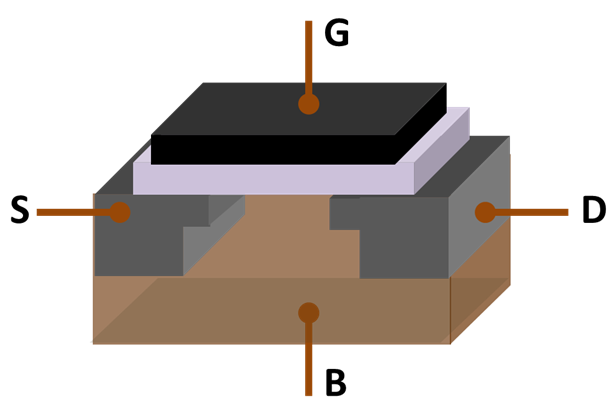
\includegraphics[width=0.5\textwidth]{mosfet}
\end{figure}

The exact details of how a MOSFET is used to construct such circuits are beyond
the scope of this thesis; we refer the interested reader to Ben Eater's videos
on the constructions~\cite{eater_making_2015}. The particularly interested
reader might also consult a standard textbook \cite{brown_fundamentals_2014} for
more on the matter. For our purposes, the upshot of this construction is that we
get, for say the NOT operation, a circuit component
\begin{center}
  \begin{circuitikz}
    \draw (0,0) node[not port] (mynot) {};
  \end{circuitikz}
\end{center}
which has low voltage on its output when it has high voltage applied to its
input, and vice versa. This behavior is precisely the equational law
characterizing the NOT operation symbol, and suggests that we interpret the
\( \top \) operation symbol as a source of high voltage and the \( \bot \) operation
symbol as a wire with no voltage applied. The AND and OR operations also enjoy
physical realizations in term of MOSFETs, as do the finite-input generalizations
of all of these operations.

The reader suspicious of abstract nonsense will complain that we have merely
dressed up in abstract nonsensical terms the well-known fact that electrical
circuits can implement combinational logic. Indeed, the utility of this example
lies not in some new exciting insight about digital circuits but rather, as we
will soon see, in leveraging our visual intuition about digital circuits to
better understand how substitution works, and why substituting for a variable is
a contravariant operation.

The circuit interpretation also provides a neat intuition for weakening.
Weakening by a variable is drawing a new input wire with the appropriate label,
and then not connecting it to anything. As an example, we have the following
equality
\begin{align*}
 \widehat{b_{4}}^{*} \bigg({\tikz[baseline=-0.5ex]{ \draw (0,0) node[and port, number inputs=3](myand){}
    (myand.in 1) node [anchor=east] {\( b_{1} \)}
    (myand.in 2) node [anchor=east] {\( b_{2} \)}
    (myand.in 3) node [anchor=east] {\( b_{3} \)};
  }}\bigg) &= \tikz[baseline=-0.5ex]{ \draw (0,0) node[and port, number inputs=3](myand){}
    (myand.in 1) node [anchor=east] {\( b_{1} \)}
    (myand.in 2) node [anchor=east] {\( b_{2} \)}
    (myand.in 3) node [anchor=east] {\( b_{3} \)}
    (myand) ++(-1.725,-.75) node[](b4){\( b_{4}\)}
    (b4) ++(1,0) node [circle,fill=black,inner sep=0pt,minimum size=7pt](myground){}
    (b4) -- (myground)
    ; }
\end{align*}
where we represent an unused input as a wire capped off with some sort of
insulating material, here displayed as a circle.

Allowing ourselves to write the operations of the algebra for the operation
symbols of the theory for a moment, consider the morphism
\[ [ \tikz{ \draw node[and port, number inputs=3](myand){} (myand.in 1) node [anchor=east] {\( b_{1} \)}
    (myand.in 2) node [anchor=east] {\( b_{2} \)} (myand.in 3) node
    [anchor=east] {\( b_{3} \)}; } \middle/ b_{4}] : [b_1 : \bitcoin,
  b_2:\bitcoin, b_3 : \bitcoin] \rightarrow [b_1:\bitcoin,b_2:\bitcoin,b_3:\bitcoin,b_4
  :\bitcoin]\] in the syntactic category. We can now consider a concrete example
of substitution in action by substituting along this morphism. Ignoring the
requisite intermediate weakenings, we have
\[
  [ \tikz{ \draw node[and port, number inputs=3](myand){}
    (myand.in 1) node [anchor=east] {\( b_{1} \)}
    (myand.in 2) node [anchor=east] {\( b_{2} \)}
    (myand.in 3) node [anchor=east] {\( b_{3} \)};
  } \middle/ b_{4}]^* (\tikz { \draw node[or port](myor){}
    (myor.in 1) node [anchor=east] { \(b_{4}\) }
  (myor.in 2) node [anchor=east] { \( b_{5}\) };}),
\]
which results in the circuit component
\[
\tikz{ \draw (0,2) node[and port, number inputs=3](myand){}
    (myand.in 1) node [anchor=east] {\( b_{1} \)}
    (myand.in 2) node [anchor=east] {\( b_{2} \)}
    (myand.in 3) node [anchor=east] {\( b_{3} \)}

    (2,0) node[or port](myor){}

    (myor.in 2) node [anchor=east] { \( b_{5}\) }
    (myand.out) -| (myor.in 1);
    }.
\]

Looking back at the morphism encoding this substitution operation, we should
remind ourselves that the \( b_{1}, b_{2}, b_{3}\) in the codomain context were
not necessarily \emph{used} in the original circuit; indeed, those variables
could be (as in this case) merely unused inputs which were added by a weakening
operation. What is essential is that such a weakening \emph{has put the input
  wires in place} before we slot the 3-wide AND into place.

\begin{definition}[$\mathcal{L}$-algebra homomorphism]\label{def:homomorphism}
  A \emph{homomorphism} \( \phi: A \rightarrow B\) of $\mathcal{L}$-algebras $A$ and $B$ in some
  category $C$ with finite-products is an assignment to each sort $X$
  of a $C$-morphism \( \phi_{X} : A_{X} \rightarrow B_{X}\) between the
  corresponding objects in each algebra such that diagrams of the following form
  commute:

  \[\begin{tikzcd}
      {A_{X_1}\times\cdots \times A_{X_k}} &&& {A_{X}} \\
      \\
      {B_{X_1}\times\cdots\times B_{X_k}} &&& {B_{X}}
      \arrow["{r_A}", from=1-1, to=1-4]
      \arrow["{r_B}", from=3-1, to=3-4]
      \arrow["{\phi_{X_1}\times \cdots \times \phi_{X_k}}"', from=1-1, to=3-1]
      \arrow["{\phi_{X}}", from=1-4, to=3-4]
    \end{tikzcd}.\]
\end{definition}

\begin{remark}\label{rmk:alg_func}
  The following is an observation due to Lawvere in a paper written in his time
  teaching at Reed College \cite{lawvere_functorial_1963}. The familiarity of
  this diagram is no mistake: indeed, by analogy to
  Theorem~\ref{thm:classify_elem_sketch}, we may understand algebras as
  product-preserving functors. A mapping between algebras then is a natural
  transformation, hence the naturality diagram in
  Definition~\ref{def:homomorphism}. We will later make this analogy more
  concrete in Theorem~\ref{thm:classifying alg theory}.
\end{remark}

\begin{remark}
  Perhaps predictably, the $C$-valued algebras and homomorphisms of
  an algebraic theory $\mathcal{L}$ form a category, called
  $\textrm{Mod}_{C}(\mathcal{L})$.
  \begin{proof}
    Per Remark~\ref{rmk:alg_func}, we consider algebras and their homomorphisms
    as functors and natural transformations respectively. The identity morphisms
    are the identity natural transformations whose component morphisms are the
    identities of $C$. Composition of natural transformations is
    given by composition of their component morphisms, hence we may out-source
    the associativity condition to that guaranteed by the categorical structure
    of $C$.
  \end{proof}
\end{remark}

Many things you'd like to prove about a type theory are concerned with the
\emph{terms} of the theory at hand. \emph{Normalization} theorems talk about the
accessibility (under some reduction relation) of a certain class of terms from
any arbitrary open term. \emph{Canonicity} or \emph{closed normalization}
theorems talk about the accessibility of a different class of terms from
arbitrary \emph{closed} terms. These are but two examples of a broad spectrum of
properties one might desire of the terms of a theory. Considering the primacy of
term properties in type theory, it is rather strange that the notion of
semantics we have built so far makes no commentary on terms besides the action
on the clones given in Theorem~\ref{thm:clone model}. Our models so far have
only given meaning to the individual \emph{sorts} (types) and individual
\emph{operation symbols} (constructors) of the theory considered. In fact, this
is enough: our models extend canonically \emph{along the product structure} to
contexts and substitutions and thus give meaning to terms.

\DeclarePairedDelimiter{\sem}{\llbracket}{\rrbracket}

\begin{definition}[Extending a model to terms]\label{def:term model}
  Let $A$ be an $\mathcal{L}$-algebra in a category $C$. This algebra
  extends canonically to an interpretation $\sem{-}$ of contexts by the
  following definition recursive in the structure of contexts:
  \begin{align}
    \label{eq:contexts interp}
    \sem{\varnothing} &= \mathbbm{1}_{C} \\
    \sem{\Gamma, x : X} &= \sem{\Gamma} \times A_{X}.
  \end{align}
  The (overly) careful reader will complain that $C$ doesn't necessarily feature
  a terminal object, but it turns out that a terminal object is
  guaranteed\footnote{I.e., because the terminal object is just the nullary
    finite product.} by the finite product closure we imposed on $C$ in our
  definition of algebras. We are good to go.

  Recalling more from the definition of an algebra, we know that $A$ gives
  meaning to each operation symbol \( Y_{1},\dots , Y_{k} \vdash r : Z \) as a
  morphism \( r_{A} : A_{Y_{1}} \times \cdots \times A_{Y_{k}} \rightarrow A_{Z} \) and gives meaning to
  each constant \( c : Z \) by a morphism \( \termob_{C} \rightarrow A_{Z} \). We can
  extend this to arbitrary terms in the context
  \( \Gamma \equiv \sem{x_{1} : X_{1}, \dots , x_{n} : X_{n}} \) by the following
  recursive definition:
  \begin{align*}\label{eq:term interp}
    \sem{x_{i}} &: \sem{\Gamma} \equiv A_{X_{1}} \times \cdots \times A_{X_{n}} \xrightarrow{\pi_{i}} A_{X_{i}} \\
    \sem{c} &: \sem{\Gamma} \xrightarrow{<_{!}} \mathbbm{1}_{C} \xrightarrow{c_{A}} A_{Z} \\
    \sem{r(u_{1}, \dots , u_{k})} &: \sem{\Gamma} \xrightarrow{\braket{\sem{u_{1}}, \dots, \sem{u_{k}}}} A_{Y_{1}} \times \cdots \times A_{Y_{k}} \xrightarrow{r_{A}} A_{Z}
  \end{align*}
  where the $\sem{u_{i}}$ are the interpretations of the sub-expressions of the
  expression in the final line, $\pi_{i}$ is the $i$th projection guaranteed to us
  by the universal property of products, and $<_{!}$ is the unique map into the
  terminal object. The angle bracket notion is used to express the product
  functor's action on morphisms in $C$. For clarity, we write out
  explicitly the composites for the reader:
  \begin{align*}
    \sem{x_{i}} &\equiv \pi_{i} \\
    \sem{c} &\equiv c_{A } \circ <_{!} \\
    \sem{r(u_{1}, \dots , u_{k})} &\equiv r_{A} \circ \braket{\sem{u_{1}}, \dots,\sem{u_{k}}}.
  \end{align*}
\end{definition}

\begin{theorem}[The classifying category of an algebraic
  theory]\label{thm:classifying alg theory}
  Let \( \mathcal{L} \) be an algebraic theory. Then $\cn_{\mathcal{L}}$ has
  finite products and
  \begin{enumerate}
    \item there exists in \( \cn_{\mathcal{L}}\) an $\mathcal{L}$-algebra which
          satisfies the following universal property:
    \item Let $C$ be another category with finite products and its
          own an $\mathcal{L}$-algebra. Then the functor
          $\sem{-} : \cn_{\mathcal{L}} \rightarrow C$ preserves finite products
          and the $\mathcal{L}$-algebra, and is the unique such functor.
  \end{enumerate}
\end{theorem}
\begin{proof}
  We first show that the syntactic category has finite products. Recall that the
  objects of the syntactic category are variable contexts
  \([x : X, y : Y, \dots]\). For any other context \( [t : T, u : U, \dots] \)
  we have the
  product \[ [x : X, y : Y, \dots] \times [t : T, u : U, \dots] = [x : X, y : Y, \dots, t : T, u : U, \dots]\]
  That is, products are given by concatenation of contexts. The projections are
  given by weakening by all the variables in either context: that is, the second
  projection is \( \Gamma \times \Delta \xrightarrow{\hat{\gamma_{1}}\circ\cdots\circ\hat{\gamma_{k}}} \Delta \) where the
  \( \gamma_{i} \) are the variables of \( \Gamma \). We define the first projection
  similarly. The universal property for products is upheld by the equational
  laws concerned with weakenings in the category of contexts.

    Now come the more interesting promised results:
    \begin{enumerate}
      \item
      \begin{enumerate}
        \item The sorts $X$ of $\mathcal{L}$ are interpreted as single variable
        contexts $[x:X] \in \ob C$ where the variable $x$ is arbitrary.
        \item The operation symbols \( X_1, X_2, \dots \vdash r : Y \) of
        $\mathcal{L}$ are interpreted as substitutions \( [r(x_1, x_2, \dots)/y] :
        [x_1:X_1, x_2:X_2,\dots] \rightarrow [y : Y]\)
      \end{enumerate}
      \item The functor promised is precisely the one defined by
      Definition~\ref{def:term model}. Preservation of the model and of
      finite products both follow from the definition of the interpretation
      by induction on contexts. Uniqueness of the functor is in turn forced
      by preservation of the model and finite products.
    \end{enumerate}
\end{proof}
\chapter[Syntax and (functorial) semantics of the lambda calculus]{Functorial
  semantics of the simply typed lambda calculus in cartesian closed
  categories}\label{chapter:stlc}
\epigraph{``Eeny, meeny, miny, moe''}{Alonzo Church (Allegedly, on his choice of
  $\lambda$ as the name for his calculus.)}

This chapter exploits the heavy machinery developed in the previous chapter to
give meaning, in specially structured categories, to the types and terms of the
simply typed lambda calculus. Here is how we shall do so: First, we will present
various a suite of simple type theories as a series of \emph{algebraic theories}
differing only in their equational laws. One of these type theories will be the
typical simply typed lambda calculus with the full gamut of equational laws,
including \( \beta \)-conversion and \( \eta \)-conversion and \( \alpha \)-renaming.
Second, we present an interesting perspective on a well known type of
categorical structure, namely \emph{cartesian closedness}, by explicitly
defining it in terms of the definitional \( \beta\) and \( \eta \) laws from type
theory. We will find that this characterization exactly coincides with the one
found in typical books on category theory. Finally, we will show that any
interpretation of base types of the simply typed lambda calculus gives rise to
an interpretation of lambda terms in any \emph{cartesian closed} category with
an interpretation of the base types. Unless otherwise noted, what follows is an
adaptation of \cite[Chapter 4.7]{taylor_practical_1999}. We begin by presenting
the term language and type system for the calculus under consideration.


\section{The simply typed lambda calculus}
We'll work with the simply typed lambda calculus with some collection $T$ of
\emph{base types} (say natural numbers, integers, booleans, or some other type
of object the reader is interested in). We will not dwell on the details of
standard aspects of this development and instead refer the reader to the
standard references \cite{pierce_types_2002}, \cite{harper_practical_2016} for
the full story.

\begin{definition}[Types]\label{def:stlc_types}
  Given a set of base types \( T\), the types \( \types \) of the simply typed
  lambda calculus are generated by the following grammar:
  \[
    \tau \Coloneqq \termob \mid \tau \rightarrow \tau \mid \tau \times \tau \mid \theta
  \]
  where \( \theta \) is a \emph{base type} drawn from \( T \). Note that the unit
  type \( \termob \) is not a base type but rather can be considered a nullary
  product of types.
\end{definition}

\begin{definition}[Terms]\label{def:stlc_terms}
  The terms of the simply typed lambda calculus (with booleans) are generated by the
  following grammar:
  \[
    t \Coloneqq x \mid () \mid \pi_{1}\, t \mid \pi_{2}\, t \mid (t_{1}, t_{2}) \mid t_{1}\, t_{2} \mid \abstr{x}{\tau}{t}
  \]
  where the variables $x$ are drawn from a countably infinite set \( V \).
\end{definition}

The typing rules are given as follows:
\begin{definition}[Typing rules]\label{def:stlc_rules}
    \begin{mathpar}
    \inferrule[]{ \Gamma \vdash t : \tau_1 * \tau_2 }{ \Gamma \vdash \pi_{i} t: \tau_{i} } \and \inferrule{ \Gamma \vdash t_{i} : \tau_{i} }{(\tau_1,\tau_{2}) : \tau_{1} * \tau_{2}}\\
    \inferrule{ \Gamma \vdash t_{1} : \tau' \rightarrow \tau  \\  \Gamma \vdash t_{2} : \tau' }{ \Gamma \vdash t_{1} t_{2} : \tau } \and \inferrule{ \Gamma,x:\tau' \vdash t : \tau}{ \Gamma \vdash \abstr{x}{\tau'}{t} : \tau' \rightarrow \tau}\\
    \inferrule*{ }{ \Gamma, x:\tau, \Gamma' \vdash x : \tau }\\
    \inferrule{ }{ \Gamma \vdash () : \termob }
  \end{mathpar}
\end{definition}

\section[Raw CCS and beta-eta is exactly CCS]{Raw cartesian closed structure, beta-eta rules, and cartesian closed structure}
The following notion mediates between \emph{having lambda abstraction} and the
more structured situation enjoyed by usual presentations of the lambda calculus.
The mediating notion, namely \emph{raw cartesian closed structure}, merely
requires that one be able to write down lambda abstractions, and that they
behave nicely with respect to substitutions that don't interfere with the bound
variable. Notably lacking in \emph{raw cartesian closed structure} from the more
structured situation referred to above are the \emph{$\beta$- and $\eta$-laws} which
explain how to \emph{compute} with lambda abstraction.
% Both the former and latter situations predictably have analogues in
% categories, in which exponential objects will serve as function types, the
% counit of the product-hom adjunction is the evaluation, and lambda abstraction
% is given by exponential transposition. We will see that the less structured

The definition comes from Taylor
\cite{taylor_practical_1999}.

\begin{definition}[Raw cartesian closed structure]
  Let \( C \) be a category with finite products together with product
  projections. We say that \( C \) is \emph{raw cartesian closed} or \emph{has
    raw cartesian closed structure} if we have the following for each pair of
  objects \( X, Y \) of \( C \):
  \begin{enumerate}
    \item An object \( Y^{X} \)
    \item A morphism, \emph{application}, \( \evsig{X}{Y} \) and
    \item For each object \( \Gamma \), a function of hom-sets
          \( \lambda_{\Gamma, X, Y} : C[\Gamma \times X, Y] \rightarrow C[\Gamma, Y^{X}] \) obeying the naturality
          law:
          \[
            \lambda_{\Gamma, X, Y} ( b \circ (u \times \id_{X})) = \lambda_{\Gamma, X, Y}(b) \circ u
          \]
          for each \( u : \Gamma \rightarrow \Delta \) and
          \( b : \Delta \times X \rightarrow Y \).
        \end{enumerate}
        Looking closely, the naturality law essentially says that substitutions
        ``not touching'' the bound variable commute with lambda abstraction.
        Informally, this is a good equation to have in mind:
        \( u^{*}(\lambda x\, . b) = \lambda x.\, (u^{*}b) \).
\end{definition}

We will say that an algebraic theory $\mathcal{L}$ \emph{has raw cartesian
  closed structure} if its classifying category \( \cnprod \) has raw cartesian
closed structure.

The following theorem extends Definition~\ref{def:term model} and shows how to
construct an interpretation of terms from an algebra in a raw cartesian closed
category. The essence is that we extend the assignments of base types and
operation symbols along products (as we did before when dealing with ordinary
algebraic theories) and along the new exponential objects as well.

\begin{theorem}\label{thm:rawccsinterp}
  Let \( \mathcal{L}\) be an algebraic theory and $C$ be a category with raw
  cartesian closed structure and an algebra for \( \mathcal{L}\). The algebra
  for \( \mathcal{L}\) extends uniquely along the raw cartesian closed structure
  to provide an interpretation of terms, which defines a functor
  \( \sem{-} : \cn_{\mathcal{L}} \rightarrow C\)
\end{theorem}
\begin{proof}
  Building on Definition~\ref{def:term model}, we define the interpretation by
  structural recursion:
  \begin{itemize}
    \item The interpretation of base types are given by the algebra for \( \mathcal{L}\)
    \item The interpretation of an exponential \( \Delta^{\Gamma}\) is
          \( \sem{\Delta}^{\sem{\Gamma}}\) where the latter is the exponential entailed by
          the raw cartesian closed structure.
    \item Contexts are taken to products as in Definition~\ref{def:term model}.
    \item The variables, operation symbols, and the laws are treated as in
          Definition \ref{def:term model}.
    \item The last clause of the raw cartesian closed structure gives the notion
          of lambda abstraction in $C$.
  \end{itemize}
\end{proof}


\begin{definition}[Beta-eta rules]
  A raw cartesian closed algebraic theory $\mathcal{L}$ satisfies the
  \emph{$\beta$-$\eta$ rules} if for all
  \( b \in \cn_{\mathcal{L}}(\Gamma \times X,Y) \) we have the equations
  \begin{align*}
    \ev{X}{Y} \circ (\lambda_{\Gamma,X,Y}(b) \times \id_{X}) &= b && (\beta) \\
    \lambda_{Y^{X},X,Y}(\ev{X}{Y}) &= \id_{Y^{X}}. && (\eta)\\
  \end{align*}
\end{definition}

These equations deserve some commentary. The beta rule says that application of
an abstracted body $b$ to the identity gives you back the body you started with:
the beta rule forces that application of lambda expressions does nothing more
than substitute for the abstracted variable. The eta rule says that taking a
function $f$, applying it to a variable $x$, then finally abstracting over that
variable $x$ is the same operation as doing nothing to $f$. We will see the more
familiar symbolic forms of these rules in the definition of the theory of the
usual calculus below.

We now define a notion more well-known outside of computing. Cartesian
closed structure endows a category with the ability to take products and
function spaces over its objects in a suitable fashion; as can be seen below,
the notion of Cartesian product and function space in the category of sets are
examples of suitable such constructions. It will turn out that this familiar
situation is equivalent to the combination of raw cartesian closed structure and
beta-eta rules.

\begin{definition}[Cartesian closed structure]
  Let \( C \) be a category. An \emph{exponential} of objects \( X \) and
  \( Y \) is an object $Y^{X}$ of \( C \) together with a morphism
  \( \epsilon : Y^{X} \times X \rightarrow Y \) such that for each object \( \Gamma \) of \( C \) and
  morphism \( b : \Gamma \times X \rightarrow Y \) there is a unique morphism
  \( \tilde{p} : \Gamma \rightarrow Y^{X} \) called the \emph{exponential transpose} such that
  \( p = \epsilon \circ (\tilde{b} \times \id_{X})\). This is a universal property: exponentials
  are unique up to unique isomorphism. A category is \emph{cartesian closed} if
  it has all finite products and all exponentials.
\end{definition}

The category \( \catset \) is the prototypical cartesian closed category whose
products are the usual cartesian products of sets and whose exponentials are
function sets: for sets $X$ and $Y$, \( Y^{X} = \{ \textrm{functions
} f \mid \textrm{dom}(f) = X \wedge \textrm{cod}(f) = Y \}\). Another good source of
example cartesian closed categories is topos theory. All elementary topoi,
including categories of presheaves, are cartesian closed
\cite{mac_lane_sheaves_1992}.

It turns out that all of these examples of cartesian closed categories can also
be characterized as raw cartesian closed categories that satisfy the beta-eta
rules.

\begin{theorem}[Finite-product category + raw CCS + beta-eta $\iff$ cartesian closed]\label{thm:rawbetaetaisccs}
  Let \( C \) be a category. Then \( C\) is cartesian
  closed if and only if \( C \) has finite products and is both raw
  cartesian closed and satisfies the beta-eta laws.
\end{theorem}

We will not repeat Taylor's proof \cite{taylor_practical_1999}, but we will say
that the proof largely comes down to these two facts: that exponential
transposes are unique and that the characterizing property of the transpose is
exactly the \( \beta \) rule.
% \begin{proof}
%   For the first direction, suppose that \( \mathfrak{C} \) is cartesian closed.
%   Then \( \mathfrak{C} \) has all exponential and all products. The map
%   \( \abstr{\Gamma}{X}{Y} : \mathfrak{C}[\Gamma\times X, Y] \rightarrow \mathfrak{C}[\Gamma, Y ^{X}]\)
%   required for raw cartesian closed structure is precisely given by the map
%   which takes the exponential transpose: \( p \mapsto \tilde{p}\). The naturality law
%   for the map is given by the product-hom adjunction. The \( \beta\) rule is the
%   universal property of the exponential transpose, and is hence satisfied.



%   required for raw cartesian closed structure. Its \emph{naturality law} is
%   precisely expressed by the naturality of the isomorphism witnessing the
%   adjunction. The \emph{application} or \emph{evaluation} map is given by the
%   counit \( \epsilon_{X,Y} : (- \times X) \circ ({-}^{X}) \rightarrow \id_{\mathfrak{C}}\) associated with
%   the above adjunction.
% \end{proof}

\section{An algebraic treatment of the lambda calculus}
Finally, we will present the lambda calculus as a series of algebraic theories,
each of which are identical except for the equations they admit. These theories
correspond to instances of the lambda calculus whose respective definitional
equalities identify more or fewer lambda terms. We will see that algebras of
these theories are essentially functors valued in specially structured
categories.

\begin{definition}[Algebraic theory of the lambda calculus]
  The \emph{$\alpha$-lambda calculus} is presented as the following algebraic theory called \( \mathcal{L}_{\lambda\alpha}\):
  \begin{enumerate}
    \item Sorts: We define the sorts to be the set \( \types \) given in
          Definition \ref{def:stlc_types}.
    \item Variables: The variables are defined as the collection
          \( \{ v : \tau \mid (v, \tau) \in V \times \types \} \) where $V$ is the countably
          infinite set $V$ of untyped variables as in
          Definition~\ref{def:stlc_terms}.
    \item We define the following operation symbols for each
          \(\tau_{1},\tau_{2},\tau,\tau' \in \types\):
          \begin{align*}
            t : \tau_{1} * \tau_{2} &\vdash \pi_{1}(t) : \tau_{1} \\
            t : \tau_{1} * \tau_{2} &\vdash \pi_{2}(t) : \tau_{2} \\
            [t_{1} : \tau_{1}, t_{2} : \tau_{2}] &\vdash (t_{1},t_{2}) : \tau_{1} * \tau_{2} \\
            \\
            [t : \tau' \rightarrow \tau , t' : \tau'] &\vdash t\, t' : \tau \\\\
            &\vdash () : \termob.\\
          \end{align*}
          The reader will note that we have not yet added an operation symbol
          for lambda abstraction. This requires careful consideration, because
          lambda abstraction is not really an operation symbol but rather a
          family of operation symbols defined mutually with the others. For each
          term \( \Gamma, x:\tau' \vdash t : \tau \), we add a new operation symbol
         \begin{align*}
           \Gamma &\vdash (\lambda x.\, t)(\overrightarrow{\gamma}) : \tau
         \end{align*}
         where $\overrightarrow{\gamma}$ is the list of variables comprising $\Gamma$.

          Finally, the complete collection of operation symbols is defined as
          the least set closed under taking abstractions in this way and
          containing the operation symbols already mentioned above.

    \item The only equation is the $\alpha$-rule which says that terms can be
          identified up to renamings of their bound variables:
          \begin{align*}
            \alphalaw. && (\alpha)
          \end{align*}

          Note that we do not include the $\beta\eta$-rules in this version.
  \end{enumerate}
\end{definition}

With this theory in hand, we first show that it is raw cartesian closed (i.e.
that it supports a reasonably coherent notion of lambda abstraction.) After
that, we will add to the theory the \( \beta\) and \(\eta \) laws. Finally, we will use
the preceding theorems to argue \emph{from $\beta$ and $\eta$} to show that the
resulting theory of the typical lambda calculus is cartesian closed.

\begin{theorem}[$\alpha$-lambda calculus is raw cartesian closed ]
  The theory \( \mathcal{L}_{\lambda\alpha}\) is raw cartesian closed
\end{theorem}
\begin{proof}
  In the following we write \( [ X \Rightarrow Y ]\) for the exponential \( Y ^{X}\), for the
  sake of legibility. The exponential
  \[{[x_{1} : X_{1},x_{2} : X_{2}\ldots, x_{j} : X_{j}]} \Rightarrow {[y_{1} : Y_{1},y_{2} : Y_{2},\ldots,y_{k} : Y_{k}]}\]
  is the context \( [f_{1} : F_{1} ,f_{2} : F_{2}, \ldots, f_{k} : F_{k}]\) where the
  \( f_{i}\) are new variables
  and \[ F_{i} = X_{1} \Rightarrow (X_{2} \Rightarrow \cdots \Rightarrow (X_{j} \Rightarrow Y_{i}) \cdots ) \] Finally, we define \(\textrm{ev}_{\overrightarrow{X},\overrightarrow{Y}} \) as
  \[ [(\cdots(f_{1}(x_{1})x_{2}) \cdots x_{j}) / y_{1}] \circ \cdots \circ [(\cdots(f_{k}(x_{1})x_{2}) \cdots x_{j}) / y_{k}] \]
  and
  \( \lambda_{\Gamma, \overrightarrow{X}, \overrightarrow{Y}} [\overrightarrow{p} / \overrightarrow{y}] \) as
  \[[(\lambda x_{1}.\,(\lambda x_{2}. \ldots (\lambda x_{k} .\, p_{1}) \ldots ))/f_{1}] \circ \cdots \circ [(\lambda x_{1}.\,(\lambda x_{2}.\, \ldots (\lambda x_{k} .\, p_{k}) \ldots ))/f_{k}].\]
  To clarify the notation, we consider a small example of an exponential object:
  the exponential
  \[ [x: X, y: Y] \Rightarrow [z: Z, w: W]\] is the context
  \[ [f_{z}: (X \Rightarrow (Y \Rightarrow Z)), f_{w} : (X \Rightarrow (Y \Rightarrow W))]. \]

  Naturality with respect to weakening and single substitution follows from the
  fact that substitution for (or weakening by) a variable $x$ commutes with
  abstraction of a distinct variable $y$: for any terms $p$ and $c$, we have
  \( [c/y]^{*} (\lambda x.\, p ) \equiv_{\alpha} \lambda x.\, ([c/y]^{*}p)\). The same situation holds
  for weakening. The full naturality law follows from this and the fact that
  single substitution and weakening are the generating morphisms of the
  syntactic category.
\end{proof}

\begin{definition}[Lambda calculus]\label{def:alpha_beta_eta_theory}
  The lambda calculus, or the $\alpha\beta\eta$-lambda calculus is defined as the algebraic
  theory of the $\alpha$-lambda calculus enriched with the following additional
  equational laws:
  \begin{align*}
    \betalaw && (\beta)\\
    \etalaw. && (\eta)\\
  \end{align*}

  We write \( \mathcal{L}_{\lambda\alpha\beta\eta}\) or simply \( \lambda \) for the new theory, and
  \( \cl \) for its classifying category.
\end{definition}

\begin{definition}[Lambda algebra]
  By a \emph{lambda algebra}, we mean an algebra for the theory
  \( \mathcal{L}_{\lambda\alpha\beta\eta}\).
\end{definition}

The following results quickly follow the definition of the theory of the lambda
calculus and the work we did in Chapter~\ref{chapter:functorial_semantics}.
\begin{theorem}
  The lambda calculus is a raw cartesian closed algebraic theory with beta-eta.
\end{theorem}

\begin{theorem}
  The syntactic category \( \cl \) of the theory \( \mathcal{L}_{\lambda\alpha\beta\eta} \) is
  cartesian closed and has a lambda algebra satisfying the following universal
  property: if $C$ is a cartesian closed category with a lambda algebra then
  there is a unique functor \( \sem{-} : \cl \rightarrow C \) that preserves the cartesian
  closed structure and the lambda algebra.
\end{theorem}
\begin{proof}
  Cartesian closure follows immediately from the previous result and
  Theorem~\ref{thm:rawbetaetaisccs}. The rest is given essentially as in
  Theorem~\ref{thm:classifying alg theory}, except that we must handle the new
  exponentials with more care. Theorem~\ref{thm:rawccsinterp} provides the
  requisite care and extends the functor defined in Definition~\ref{def:term
    model} to provide one which preserves exponentials as required.
\end{proof}

This final result will prove important in Chapter~\ref{chapter:gluing}.

\chapter{Normalization by gluing}\label{chapter:gluing}
\epigraph{You, you were like glue\\
  holding each of us together\\
  I slept through July\\
  while you made lines in the heather}{Fleet Foxes, ``Lorelai''}

The next two chapters will consider the normalization problem for the simply
typed lambda calculus using the technology we've developed so far. We begin by
reviewing the notion of normalization most likely to be familiar to the reader.
Normalization\footnote{As we will note below, we are talking about an
  \emph{operational} characterization of normalization here.} comes in both weak
and strong flavors, but both are properties of a \emph{reduction} relation, say,
\( - \rightarrow = \) defined over the terms of a theory. By a \emph{normal form} we mean
a term $t$ for which there is no other $t'$ such that \( t \rightarrow t' \). Writing
\( - \rightarrow^{*}\, = \) for the least transitive, reflexive closure of this relation,
we say the reduction system enjoys \emph{weak normalization} if for any
well-typed term \( e \), there exists a normal form \( n \) such that
\( e \red n\). A reduction system enjoying \emph{strong normalization} is one
for which \emph{every} reduction sequence ends in a normal term. These are
\emph{operational} characterization of normalization; we will see below
\emph{equational} characterizations of normalization that better line up with
what we have done so far.

Theorems \emph{about theories} (such as a programming language or type system)
are called \emph{metatheorems}. Normalization theorems, then, are
\emph{metatheorems}. Type safety\footnote{This result is often sloganized as
  \emph{well-typed (closed) terms don't go wrong}.} is another class of
metatheorem which is much more famous than normalization, perhaps because some
of its variants enjoy straightforward proofs. One variant of this result called
\emph{syntactic type safety} defines a set of chosen \emph{good terms} called
values and defines a \emph{stuck term} to be a term which is both irreducible
and \emph{not} a value. The syntactic type safety theorem says that well-typed
terms \( \Gamma \vdash t : \tau \) never reduce to a stuck term. This variant of type safety
enjoys a straightforward proof by induction over typing derivations using a
trick called \emph{progress and preservation}. See Chapters 8 and 9 of Pierce's
textbook \cite{pierce_types_2002} for the details.

Normalization theorems on the other hand tend to resist standard techniques like
straightforward induction over typing derivations. A famous example is
\emph{closed normalization} which says that all closed terms have a normal form.
When easy induction fails, metatheoreticians resort to \emph{occult} techniques
like the method of logical relations. The method of logical relations is,
broadly speaking, opaque to all but its most experienced practitioners. In
short, a logical relation is a relation of terms indexed by the types of the
theory whose inclusion criteria in some vague sense mirror the type structure of
the theory. Such logical relations are easy to work with in simple settings like
that of the closed normalization problem for the simply-typed lambda calculus,
see Pierce's textbook \cite{pierce_types_2002}. However, logical relations are
well known to become fiendishly complicated when working with theories whose
type structure is more complicated. Examples of such complexity include the
addition of type system features associated with computational effects, such as
\emph{recursive types} (the effect being non-termination) or \emph{mutable
  reference types} (the effect being change of \emph{state}). Another variant of
type safety presents a great example of the problems associated with using
logical relations in the presence of these features.

Type safety has another characterization called \emph{semantic type safety}, as
espoused by Milner in his paper introducing the concept of type safety
\cite{milner_theory_1978}. Proving semantic type safety involves building a
\( \catset \)-valued model $A$ of the type theory in question where the sets
$\sem{\tau}_{A}$ of the model are comprised of terms satisfying a certain
behavioral requirement. With this done, a \emph{semantic typing} relation
\( \Gamma \Vdash t : \tau \) is defined by \( t \in \sem{\tau}_{A} \). Finally, one proves the
so-called \emph{fundamental} theorem which says that all \emph{syntactically}
well-typed terms \( \Gamma \vdash t : \tau \) are also \emph{semantically} well-typed, so
that all \emph{syntactically} well-typed terms satisfy the behaviorally
properties for their type as specified in the model. This type of result is
unlike \emph{syntactic} type safety in that it does not admit easy proofs by
induction on typing derivations, and rather are typically proven with logical
relations. This is no problem for well-behaved type systems like the simply
typed lambda calculus, but for type systems with features like \emph{mutable
  reference types} even (ordinary) logical relations don't suffice and more
advanced proof techniques are required. The additional heavy machinery called
for is the method of \emph{step-indexed logical relations}, a form of
\emph{Kripke logical relations} which I describe below and detail in this
chapter. Ahmed, for example, employed \emph{step-indexed logical relations} to
prove for the first time the semantic type safety of a version of System F
endowed with mutable reference types in her doctoral thesis
\cite{ahmed_semantics_2004}.

It is not just realistic programming languages whose metatheory demands the use
of such heavy machinery, however. The very nature of certain metatheoretical
problems preclude the use of ordinary logical relations. One such problem is the
\emph{open normalization} problem for the simply typed lambda calculus. Open
normalization generalizes the closed normalization problem to terms with free
variables: we require that every well-typed term \( \Gamma \vdash t : \tau \) has a normal
form, in the same sense as above. Such problems again demand that the logical
relation be indexed not just by types, but also by the elements of some poset
\cite{harper_kripke-style_nodate}. That poset might be, as in the case of the
open normalization problem, the poset of contexts \( \Gamma \) ordered by weakenings
\( \hat{x}\). Such a relation indexed by a poset is called a Kripke relation if
it additionally satisfies a certain monotonicity condition. In the example of
the previous sentence, these conditions amount to saying that a term which has a
normal form when considered as a term under the context \( \Gamma \) should also have
a normal form when considered as a term under any extended context
\( \Gamma, x', \dots, z'\). In the case of \emph{step-indexed logical relations}, the
indexing poset is \( \mathbb{N} \) where the indices represent \emph{remaining
  reduction steps} and the partial order \( m \leq_{\texttt{step}} n \) is defined
e as \( n \leq m \). That is not a typo. The monotonicity condition, then, says
that a term is in the relation when allowed $k$ steps of reduction is also in
the relation when allowed \emph{fewer} steps of reduction
\cite{benton_formalizing_2007}. Don't read too much into this; we will be
working with something closer to the poset of contexts ordered by weakenings
mentioned before.

This chapter will consider the open normalization problem for the simply typed
lambda calculus from a slightly different perspective. First of all, the problem
we will tackle is not exactly the one I suggested at the beginning of this
introduction. Instead of an \emph{operational} normalization theorem, we seek to
prove an \emph{equational} normalization theorem, in keeping with the
perspective we developed in the previous two chapters. The \emph{equational}
version of the normalization problem asks for a given well-typed term
\( \Gamma \vdash t : \tau \) whether there exists a normal form \( N \) such that
\( \sem{t} = \sem{N}\), i.e., the two are equal as morphisms in the syntactic
category. In fact, our solution will offer even more than that, giving a
\emph{function} which computes the corresponding normal form for a given term.
Our methods are also substantially different from the usual approach. Building
on our work in the previous two chapters, we will develop and make use of the
category-theoretic \emph{Artin gluing} construction to tackle this problem.
Briefly, the gluing construction allows us to define a category of \emph{proof
  relevant Kripke logical predicates}, meaning that the objects of the category
are Kripke predicates (in the sense of Kripke logical relations mentioned above)
with a twist: just as a category is a proof-relevant poset (i.e., morphisms
\( a \rightarrow b \) are witnesses for the proposition \( a \leq b \)) a proof relevant
Kripke logical predicate is one where any inhabitant of the predicate can have
multiple \emph{witnesses} of its membership. The predicates are \emph{logical}
insofar as the category is \emph{cartesian closed}, which the reader will
recognize as saying that it in some sense mirrors the type structure of the
lambda calculus.

Where the method of Kripke logical relations is ad-hoc and mysterious, gluing
regularizes the thought involved and delivers more conceptual proofs and theory.
The gluing construction is perhaps overshadowed in fame by one of its instances:
The \emph{scone} or \emph{Sierpinski cone} is well-known outside of type
theoretic circles for its use in proving results similar to closed
normalization. Because we are interested in open normalization, the scone
construction is not suited to the problem at hand. The reader interested in the
broader context is encouraged to read on in Section 22 of Part II of Lambek and
Scott's \emph{Introduction to higher order categorical logic}
\cite{lambek_introduction_1989}. Our own case will involve an instance of the
gluing construction which, in some sense, glues the syntax of open terms to its
meaning in the semantics (in the category \( \cl \)). The gluing construction is
set up exactly so that morphisms in the category are pairs of \emph{syntactic
  transformations} and \emph{semantic transformations} (namely substitutions)
which in some sense commute with the semantic interpretation of terms in
\( \cl \). Our normalization function then will be delivered from a composite of
these morphisms, so that the semantic equivalence of the input term and the
computed normal form is essentially automatic once we have verified that the
maps involved in the composite are genuine morphisms of the gluing category. In
this sense, the gluing category we work with has been set up not just to mirror
the type structure of the simply-typed lambda calculus, but to also mirror the
desired result.

This chapter will develop the gluing construction itself and define our
particular gluing category. There is a lot of technology to build up, and many
of the constructions we'll see are non-trivial. \emph{Math is hard, but we'll
  get through it together!} The subsequent chapter will leverage the technology
of this chapter to deliver the long-promised normalization function.

\section{The comma construction and friends}
This section introduces a general construction that will, among other things,
allow us to define the gluing construction from which this chapter gets its
name. The loose idea of the comma construction is to glob some extra data to the
objects of a category in a way that supports a well-defined notion of an
object-with-extra-data-morphism which preserves the attached data. This
intuition perhaps underlies the name for the gluing construction. Our specific
use of the gluing construction will involve gluing presheaves of syntactic terms
(as you would write them down on paper) together with presheaves of semantic
terms (which are \emph{substitutions}.) That is, the extra data we glob on is
the semantics of terms, and the notion of extra-data-preserving morphism is a
pair of a syntactic transformation and a substitution which commute with the
semantic interpretations of the syntax.

\begin{definition}[Comma category]
  Let $E,D,C$ be categories and \[F: D \rightarrow C \leftarrow E : G \] be a pair of functors sharing
  their codomain $C$. The comma category \( F \downarrow G \) has as its
  \begin{enumerate}
    \item Objects: triples \( (d : D, Fd \xrightarrow{f} Ge, e : E) \)
    \item Morphisms: $(h,k) : (d, f, e) \rightarrow (d', f', e')$ are pairs of $D$ and
          $E$-morphisms \(h : d \rightarrow d', k : e \rightarrow e'\) making the following diagram
          commute:
          \[
            \begin{tikzcd}
              Fd \arrow{r}{Fh} \arrow{d}[swap]{f} & Fd' \arrow{d}{f'} \\
              Ge \arrow{r}[swap]{Gk} & Ge'\\
            \end{tikzcd}
          \]
  \end{enumerate}

\end{definition}

\begin{remark}[The gluing construction]
  When in the above we have $D=C$ and $F = \id_{C}$, we will write \( C \downarrow G\)
  for the comma category and we will say that we have \emph{glued $C$ to $E$
    along $G$}.
\end{remark}

\section{An easy instance of the comma construction: the category of renamings}
As a warm-up example, we present the \emph{category of renamings} which can be
nicely expressed as an instance of the comma construction. In elementary terms,
the category has the same objects as the syntactic category (i.e., contexts) but
the morphisms are a restricted class of substitutions, which are only allowed to
substitute for a variable \emph{by a variable of the same type} or weaken by a
variable. Thus the category of renamings is something like a less proof-relevant
version of the category of contexts and substitutions in the following sense: if
there exists a substitution relating two contexts in the syntactic category,
then there exists a renaming relating the same contexts. The upshot is that
renamings allow us to track changes in context \emph{due to a substitution}
without actually working with substitutions directly. Working over \( \cl \) is
problematic because substitutions (and thus the terms they represent) are
identified up to computational equality, whereas we would like to distinguish
between terms at differing stages of reduction (e.g. distinguishing between a
term and its normal form.) We will understand this problem in greater detail in
Remark~\ref{rmk:syntactic-cat-bad}. Concisely, the category of renamings allows
us to define the presheaves we need while not losing track of how contexts
evolve by substitution\footnote{The reader might complain now, as I did, that if
  we only care about tracking how contexts evolve by substitutions then we
  should simply work with the category of context \emph{weakenings}. The problem
  here is that the category of weakenings lacks finite products, which precludes
  the use of a trick (which we will soon see \emph{does} work in the case of the
  category of renamings) for explicating the binding structure of its category
  of presheaves. Thank you to Carlo Angiuli for explaining this to me!}. We
present the category abstractly as a comma category and at the same time spell
out concretely its morphisms in terms of the substitutions of the syntactic
category:
\begin{definition}[Category of renamings]
  Recall from Chapter~\ref{chapter:stlc} that \( V \) is some countably infinite
  set of variables and \( \types \) is the set of all types in the simply typed
  lambda calculus generated from a set of base types \( T \). Let \( \fin \) be
  the category whose objects are finite subsets of \( V \) and whose morphisms
  are all functions between the underlying sets. Let
  \( \mathbb{T} : \termob_{\mathfrak{Cat}} \rightarrow \catset \) be the functor sending
  the single object of the terminal category to the set \( \types\). Let
  \( U : \fin \rightarrow \catset \) be the forgetful functor taking finite variable sets
  to their underlying sets and functions to functions. Now by the \emph{category
    of renamings} we mean the \emph{opposite category} of the comma category
  \( U \downarrow \mathbb{T} \) whose
  \begin{itemize}
    \item Objects are \emph{pairs} \( (V : \fin, \Gamma : V \rightarrow \types) \), i.e.,
          finite variable list together with an assignments of types to a each
          variable. Note that we elide the final entry of the triple, since it
          is always the object \( * : \termob_{\mathfrak{Cat}}\) and is
          therefore uninformative. These objects are precisely the contexts of
          the familiar classifying category.
    \item Morphisms of contexts \( (V , \Gamma) \rightarrow (V', \Gamma')\) are functions
    \( \rho : V \rightarrow V' \) making the following diagram commute:
    \[
      \begin{tikzcd}
        V \arrow{d}[swap]{\Gamma} \arrow{r}{\rho} & V' \arrow{d}{\Gamma'} \\
        \types \arrow{r}[swap]{\id_{\types}} & \types\\
      \end{tikzcd}.
    \]
    The reason the morphisms are single functions and not pairs is that
    the second function would not communicate any data, it would simply be
    taken by \( \mathbb{T}\) to the identity no matter what it is. We now
    unpack what this means. The functions \( \rho \) are
    \emph{type-preserving renamings}: for each variable \( x \in V\), we
    have that \( \Gamma'(\rho x) = \Gamma(x)\). In particular, this restricts \( \rho \)
    to the following classes of morphisms in the classifying category:
    substitutions of variables for variables of the same type, context
    extension with new variables, and all compositions of these. The
    equations are given by the substitution lemma, as in the syntactic
    category.
  \end{itemize}

  We write \( \ren = (U \downarrow \mathbb{T})^{\textrm{op}}\) for the category of
  renamings.
\end{definition}

\begin{remark}\label{rmk:reninclusioncl}
  We write for the functor \( \iota : \ren \rightarrow \cl \) which takes contexts to contexts
  and casts renamings as change-of-variable (or weakening) substitutions. When
  going between \( \ren \) and \( \cl \), we will take the liberty to implicitly
  insert this coercion as needed without further warning. It turns out that this
  functor is \emph{faithful} and thus witnesses \( \ren \) as a
  \emph{subcategory} of the syntactic category.
\end{remark}

\section{Variable-arity Kripke relations}
In order to motivate the next example of a comma construction, we will define
\emph{variable-arity Kripke relations}. Variable-arity Kripke relations are,
loosely speaking, families of relations parameterized by the objects of some
\emph{category} (c.f. the Kripke logical relations mentioned in the
introduction, which vary over the objects of a \emph{poset}) for which inclusion
in the relations respects, in a sense to be defined, the morphisms of that
category.
\begin{definition}[$C$-Kripke relation]
  Let $C$ and $S$ be categories. For a functor \( \varsigma : C \rightarrow S \), a
  \emph{$C$-Kripke relation} $R$ of \emph{arity} $\varsigma$ over an object \( A \) of
  \( S \) is a family of sets \( \{ R(c) \subseteq S(\varsigma(c), A)\}_{c \in C}\) satisfying the
  following \emph{monotonicity} condition:

  For each morphism \( \rho : c' \rightarrow c \) in \( C \) and every \( a : \varsigma(c) \rightarrow A \) in
  $R(c)$, the map \( a \circ \varsigma(\rho) : \varsigma(c') \rightarrow A\) is in $R(c')$.
\end{definition}

In order to disentangle this admittedly abstract definition, we specialize to
the case of \( \ren\)-Kripke relations which are perhaps more graspable.

\begin{example}[A class of \( \ren \)-Kripke relations over \( \cl \)]
  Consider the inclusion functor \( \iota : \ren \rightarrow \cl \). Following the definition
  above, we can define a \( \ren\)-Kripke relation $R$ of \emph{arity} $\iota$ over
  any type\footnote{Remember that a type is in particular a singleton context.}
  \( \tau \) of \( \cl \) by producing a family of sets
  \( \{ R(\Gamma) \subseteq \cl[\Gamma, \tau]\}_{\Gamma \in \ren}\), namely a selection of terms of type
  \( \tau \) in each context \( \Gamma \), along with a proof of the monotonicity
  condition: for each \emph{renaming} \( \rho : \Gamma' \rightarrow \Gamma \) in \( \ren \) and every
  \emph{term} \( t : \Gamma \rightarrow \tau \) in $R(\Gamma)$, the map \( t \circ \iota(\rho) : \Gamma' \rightarrow \tau\) is in
  $R(\Gamma')$. This example demonstrates that we can think of Kripke relations as
  families of unary relations for which inclusion in any of the relations in the
  family, say $R(\Gamma)$, those unary relations of terms which can be
  \emph{lifted} along a renaming to yield a proof of inclusion in the relation
  at any other context \( \Gamma' \) enjoying a renaming into \( \Gamma \).
\end{example}

Even with a more concrete example, it can be hard to understand what the utility
of a construction like this is without knowing how to map between such
$C$-Kripke relations of a given arity. In fact, we will not say explicitly what
a $C$-Kripke morphism is at all. Instead we turn directly to the work of
defining the \emph{gluing category} which turns out to generalize $C$-Kripke
relations to \emph{proof relevant Kripke logical predicates}. Indeed, there is a
a category of $C$-Kripke relations whose objects are defined as above; that
category can be found to be a full subcategory of the gluing category which we
introduce next. We refer the reader to \cite{fiore_semantic_2002} for more
commentary on this result and for a more detailed treatment of Kripke relations
in general.

\section{A harder comma category: the gluing category; or, Artin's monster}
With the category of renamings in hand, we can now define \emph{by the comma
  construction} the gluing category. To define it, we first need to define a
functor along which to take the comma. In a loose sense that will be explained
in due course, this functor defines \( \ren \)-presheaves of \emph{open}
(semantic) terms.
\subsubsection{The relative hom functor}
Every functor \( \varsigma : \mathcal{R} \rightarrow \mathcal{S} \) induces the following
situation:

% https://q.uiver.app/?q=WzAsNSxbMCwwLCJcXG1hdGhjYWx7Un0iXSxbMiwwLCJcXG1hdGhmcmFre1NldH1ee1xcbWF0aGNhbHtSfV5cXHRleHRybXtvcH19Il0sWzAsMSwiXFxtYXRoY2Fse1N9Il0sWzIsMSwiXFxtYXRoZnJha3tTZXR9XntcXG1hdGhjYWx7U31eXFx0ZXh0cm17b3B9fSJdLFsxLDBdLFswLDIsIlxcdmFyc2lnbWEiLDJdLFsyLDMsIuOCiCIsMix7InN0eWxlIjp7InRhaWwiOnsibmFtZSI6Imhvb2siLCJzaWRlIjoiYm90dG9tIn19fV0sWzIsMSwiXFxicmFrZXR7XFx2YXJzaWdtYX0iLDAseyJzdHlsZSI6eyJib2R5Ijp7Im5hbWUiOiJkYXNoZWQifX19XSxbMywxLCJcXHZhcnNpZ21hXioiLDJdXQ==
\[\begin{tikzcd}
	{\mathcal{R}} & {} & {\mathfrak{Set}^{\mathcal{R}^\textrm{op}}} \\
	{\mathcal{S}} && {\mathfrak{Set}^{\mathcal{S}^\textrm{op}}}
	\arrow["\varsigma"', from=1-1, to=2-1]
	\arrow["{よ}"', hook', from=2-1, to=2-3]
	\arrow["{\braket{\varsigma}}", dashed, from=2-1, to=1-3]
	\arrow["{\varsigma^*}"', from=2-3, to=1-3]
\end{tikzcd}.\]

That is, we get a functor
\[
  \braket{\varsigma} : \mathcal{S} \rightarrow \mathfrak{Set}^{\mathcal{R}^{\textrm{op}}}
\]
by adjusting the Yoneda embedding into the category of $\mathcal{S}$-presheaves.
Specializing to the case of the inclusion \( \iota : \ren \rightarrow \cl \) of
Remark~\ref{rmk:reninclusioncl} gives us a functor
\begin{align*}
  \mathfrak{Tm} : \cl &\rightarrow \renhat \\
  \Delta &\mapsto \cl(\iota(-), \Delta) \\
\end{align*}

where \( \renhat \) is the category \( \mathfrak{Set}^{\ren^{\textrm{op}}} \).
This functor can be construed as taking a syntactic context to a presheaf of
open terms. This is a confusing idea at first, and it helps to consider the
simple cases to understand it. Consider any singleton context \( \tau : \cl \).
$\tm$ takes $\tau$ to the presheaf \( \cl(-, \tau)\) which takes any renaming context
\( \Gamma \) to \( \cl(\Gamma, \tau)\). Recalling the definition of the syntactic category
and its generating morphisms, the latter set comprises the terms of type \( \tau \)
closed under $\Gamma$, represented as single substitutions \( [t/x] : \Gamma \rightarrow \tau \).
Generalizing to multivariable target contexts \( \Delta \) gives presheaves of
\emph{lists} of open terms of the types in $\Delta$.

It turns out that the category of \( \ren\) presheaves shares the cartesian
closed structure of \( \cl \) and that \( \tm \) preserves this structure.
\begin{remark}\label{rmk:tm-cartesian-closed}
  Any category of presheaves, including \(\renhat\), is cartesian closed.
  Furthermore, the relative hom functor is a \emph{cartesian closed functor},
  meaning that for contexts \( \Gamma \) and \( \Delta \) we have the following
  isomorphisms of presheaves:
  \begin{enumerate}
    \item \(  \tm(\Gamma) \times \tm(\Delta) \cong \tm(\Gamma \times \Delta) \)
    \item \( {\tm(\Gamma)}^{\tm(\Delta)} \cong \tm(\Gamma^{\Delta}) \)
  \end{enumerate}

  We write \[ \tm(\Gamma) \times \tm(\Delta) \xrightarrow{i_{\pi}} \tm(\Gamma \times \Delta)\] for the first
  isomorphism and \[ \tm(\Gamma)^{\tm(\Delta)} \xrightarrow{i_{e}} \tm(\Gamma^{\Delta} )\] for the
  second.

  The reader should consult Chapter 8 of Awodey's \emph{Category Theory}
  \cite{awodey_category_2010} for more information about these results.
\end{remark}

\subsubsection{Gluing syntax to semantics along the relative hom functor}
We at last define the \emph{gluing category} as the comma category of the
category of renamings taken along the relative hom functor \( \tm \) just
defined.

\begin{definition}[The gluing category]
  The gluing category \( \gl \) is defined as the comma category
  \( \renhat \downarrow \tm \). Explicitly, its objects are triples
  \[ (R : \renhat, q : R \Rightarrow \tm(\Delta), \Delta : \cl). \] The objects of the gluing
  category are \emph{proof relevant Kripke logical predicates}, in a sense that
  will be more clear after a digression to follow. Following the definition of
  the comma construction, the morphisms \( (R, q, \Delta) \rightarrow (R', q', \Delta') \) are pairs
  $(d : R \rightarrow R', \delta: \cl(\Delta', \Delta))$ of a $\renhat$ natural transformation and a
  substitution making the following diagram commute:
  % https://q.uiver.app/?q=WzAsNCxbMCwwLCJEIl0sWzIsMCwiRCciXSxbMCwyLCJcXG1hdGhmcmFre1RtfShcXERlbHRhKSJdLFsyLDIsIlxcbWF0aGZyYWt7VG19KFxcRGVsdGEnKSJdLFswLDEsImQiXSxbMiwzLCJcXG1hdGhmcmFre1RtfShcXGRlbHRhKSJdLFswLDIsInFfe1xcRGVsdGF9IiwyXSxbMSwzLCJxX3tcXERlbHRhJ30iXV0=
  \[\begin{tikzcd}
      R && {R'} \\
      \\
      {\mathfrak{Tm}(\Delta)} && {\mathfrak{Tm}(\Delta')}
      \arrow["d", from=1-1, to=1-3]
      \arrow["{\mathfrak{Tm}(\delta)}", from=3-1, to=3-3, swap]
      \arrow["{q}"', from=1-1, to=3-1]
      \arrow["{q'}", from=1-3, to=3-3]
    \end{tikzcd}.
  \]

  We will refer to objects and morphisms in the gluing category as \emph{glued
    objects} and \emph{glued morphisms} respectively. We do not have a great
  name for the maps \( q : R \Rightarrow \tm(\Delta) \) that form part of the data of a glued
  object. In practice, these maps will often be the semantic interpretation of
  syntactic terms in \( \cl \), so for glued objects in general we will call
  \( q \) the \emph{interpretation} even if $q$ is not necessarily the usual
  semantic interpretation.
\end{definition}

We can get a foothold understanding of the objects of the gluing category by
considering them as a presheaf together with, for each \( \Gamma \), an
\emph{interpretation} \( q_{\Gamma} \) of each element in \( R(\Gamma)\) as a semantic
term in \( \tm(\Delta)(\Gamma) = \cl(\Gamma,\Delta)\) such that the interpretation commutes with
renamings in a way that will be further explained in just a bit.

Holding off our desire to further understand the objects, we can already
understand the morphisms. A morphism \( (d, \delta) \) is a natural transformation of
\(\ren \)-presheaves glued together with a substitution, such that performing
on \( R \) the transformation \( d \) and then looking at the \emph{semantics}
of the resultant presheaf \( R' \) by interpreting along \( q' \) is the same as
interpreting the semantics of the original presheaf \( R \) along \( q \) and
then performing a semantic transformation by substituting with \( \delta \). This
intuition will become more clear when we define glued objects over
\emph{presheaves of syntax} for which the interpretation \( q : R \Rightarrow \tm(\Delta)\) is
the actual \emph{interpretation of syntax} in the classifying category.

We can now better understand the objects by understanding how the gluing
category subsumes the notion of variable-arity Kripke relations.

\subsubsection{The subcategory of (ordinary) variable-arity Kripke relations}
We can recover ordinary, proof-\emph{irrelevant} variable-arity Kripke relations
as a subcategory of the gluing category. In particular, ordinary variable-arity
Kripke relations arise as those objects
\( (D : \renhat, q : D \Longrightarrow \tm (\Delta), \Delta : \cl) \) of the gluing category whose
interpretation map $q$ is a component-wise monomorphism; i.e., for each
\( \Gamma \in \ren \), we have that \( q_{\Gamma} : D(\Gamma) \rightarrowtail \tm (\Delta)(\Gamma) \) is a monomorphism.
Here's why: recalling the definition of $\ren$-Kripke relations over $\tau \in \cl$,
we need to find in these data a $\ren$-indexed family \( \{ R_{\Gamma}\}_{\Gamma \in \ren}\)
of sets of $\cl$-morphisms into \( \tau \) subject to the following monotonicity
condition: for any renaming \( \rho : \Gamma' \rightarrow \Gamma \), if \( t : \Gamma \rightarrow \tau \) is in
\( R_{\Gamma}\), then we have that \( t \circ \rho : \Gamma' \rightarrow \tau \) is in \( R_{\Gamma'}\). Looking
again to our proposed Kripke predicate objects of the gluing category, we can
see that the presheaf \( R \) together with the natural mono \( q \) define for
each \( \Gamma \) a subset of the substitutions \( \Gamma \rightarrow \tau \). It is tempting to
dismiss the naturality of $q$ as bureaucracy, but naturality turns out to be
essential to recovering the monotonicity condition. To see this, we need to look
at the naturality diagram of \( q \):

  \[\begin{tikzcd}
      {R (\Gamma)} &&& {\tm(\Delta) (\Gamma)} & t \\
      \\
      {R (\Gamma')} &&& {\tm(\Delta) (\Gamma')} & {t \circ \rho}
      \arrow["{q_{\Gamma}}", from=1-1, to=1-4, rightarrowtail]
      \arrow["{q_{\Gamma'}}", from=3-1, to=3-4, rightarrowtail,swap]
      \arrow["{R (\rho)}"', from=1-1, to=3-1]
      \arrow["{\tm(\Delta) (\rho)}", from=1-4, to=3-4]
      \arrow[from=1-5, to=3-5, mapsto]
    \end{tikzcd}.
  \]

  As mentioned before, because the components \( q_{\Gamma}\) of the interpretation
  are monos we may identify the component morphisms with their images. We write
  \( |q_{\Gamma}| \subseteq \tm(\Delta)(\Gamma) \) for the image, for each \( \Gamma \). Now what this
  diagram says is that for any \( q_{\Gamma }(r \in R(\Gamma)) = t \in |q_{\Gamma}|\), we have that
  \( t \circ \rho = q_{\Gamma'}(R(\rho)(r)) \in |q_{\Gamma'}|\). This is precisely the monotonicity
  condition for $\ren$-Kripke relations over \( \Delta \): containment in each
  predicate is functorial with respect to renaming \emph{up to renaming}.

  The perspective gained above allows for a more conceptual understanding of the
  objects in the gluing category: the presheaves $R$ define context-indexed
  families of \emph{witnesses} to the inclusion of terms in the predicate, and
  each \( q_{\Gamma}\) is a quotient map \emph{into its image} that forgets the
  difference between distinct witnesses \( w, w' \in R(\Gamma) \) and whose image just
  records those terms \( t \in \tm (\Delta)(\Gamma)\) taken to be in the predicate; insofar
  as $q$ is a mono, these objects are exactly variable-arity Kripke relations
  over the context \( \Delta \).

\chapter{Obtaining a normalization function}\label{chapter:normalization}
\epigraph{I stood on wondering which way to go\\
I lit a cigarette on a parking meter\\
And walked on down the road, it was a normal day
}{Bob Dylan}
\section{Presheaves of neutral and normal syntax}
In this section, we will enlist a motley crew of \emph{presheaves of syntax}
which more-or-less represent certain classes of terms in the lambda calculus.
These presheaves are defined over $\ren$ rather than $\cl$ for reasons that will
be detailed in Remark~\ref{rmk:syntactic-cat-bad}. We will ultimately define
lambda algebras over these presheaves, for which we require some understanding
of how to represent variables in $\renhat$ and how exponentiation in $\renhat$
corresponds to lambda abstraction.
\subsection{Variables and binding in Renhat}
\begin{definition}[Variable presheaf]\label{def:varpsh}
  We can define a presheaf of \emph{typed variables} in $\renhat$ with the Yoneda embedding on $\ren$:
  \[
    \mathfrak{V}_{\tau} = \yoneda \tau = \ren(-, \tau).
  \]

  With that definition, we have \( \varpsh(\Gamma) = \ren(\Gamma,\tau) \) where the
  right-hand side is comprised of renamings \( \Gamma \rightarrow [x:\tau]\) which are
  \emph{functions} \( \rho : \dom([x:\tau]) \rightarrow \dom(\Gamma)\) such that
  \( \Gamma(\rho(x)) = [x : \tau](x) = \tau\). That is, the \( \rho \) are functions selecting a
  variable of type $\tau$ in \( \Gamma \). More concisely, we have an isomorphism
  \( \varpsh(\Gamma) \cong \{ x \mid (x:\tau) \in \Gamma \}\) by which we allow ourselves to consider
  this a \emph{presheaf of syntax}.
\end{definition}

The Yoneda lemma delivers the following insight about a special class of
exponential objects in \( \renhat \). Let \( \mathfrak{P} : \renhat \).
Exponentiation by a representable/variable presheaf, \( \varpsh = \yoneda \tau\)
gives

\begin{align*}
  \mathfrak{P}^{\mathfrak{V}_{\Delta}}(\Gamma)  &= \mathfrak{P}^{\yoneda \tau}(\Gamma) \\
                                      &= \renhat[\yoneda \Gamma \times \yoneda \tau, \mathfrak{P}] && (2)\\
                                      &\cong \renhat[\yoneda (\Gamma \times \tau), \mathfrak{P}] && (\textrm{since the Yoneda embedding is cartesian closed}) \\
                                      &\cong \mathfrak{P}(\Gamma\times\tau). && (\textrm{by the Yoneda lemma})\\
\end{align*}

Where step (2) follows from the definition of the exponentials in the category
of presheaves, c.f. page 46 of \cite{mac_lane_sheaves_1992}.

The presheaves of typed variables together with the simplified view of
variable-exponentiation in $\renhat$ will allow us to more easily define
algebras for a new algebraic theory \( \NN \) of stratified \emph{neutrals and
  normals}, which allows for a more fine-grained discussion of normal terms.

\subsection{Stratifying neutral and normal terms}
We introduce a new type system over the syntax and type structure of the lambda
calculus as defined in Chapter~\ref{chapter:stlc}. This new type system will
distinguish between \emph{neutral terms} and ordinary normal terms. The
\emph{neutral terms} are a special class of \emph{normal terms} which are in
some sense terms who might otherwise be reducible if not for having a variable
as a subterm of an elimination form. Put another way, \emph{neutral terms} can
be regarded as those terms which may only be normal because they are waiting on
the value of a variable.

\begin{definition}[Neutral and normal judgments]\label{def:neut-norm-rules}
  \begin{mathpar}
    \inferrule*[Right={ \( (x:\tau) \in \Gamma \) }]{ }{ \Gamma \vdash_\neu x : \tau }\\
    \inferrule{ \Gamma \vdash_\neu M : \tau_1 * \tau_2}{\Gamma \vdash_\neu \pi_i M : \tau_i} \and \inferrule{ \Gamma \vdash_\neu t_{1} : \tau' \rightarrow \tau  \\  \Gamma \vdash_\nf t_{2} : \tau' }{ \Gamma \vdash_\neu t_{1} t_{2} : \tau } \\

    \inferrule{}{ \Gamma \vdash_\nf () : \termob } \and \inferrule{\Gamma \vdash_\nf N_i : \tau_i}{\Gamma \vdash_\nf (N_1, N_2) : \tau_1 * \tau_2} \and \inferrule{\Gamma, x : \tau \vdash_\nf b : \tau' }{\Gamma \vdash_\nf \abstr{x}{\tau}{b} : \tau \rightarrow \tau'} \\
    \inferrule*[Right={ ($\theta \in T$ $\textrm{a base type}$) }]{\Gamma \vdash_\neu t : \theta}{\Gamma \vdash_\nf t : \theta} \\
  \end{mathpar}
\end{definition}

\begin{definition}[Algebraic theory of neutrals and normals]\label{def:theory_neut_norm}
  The judgments above suggest the definition of a theory with a richer sort
  structure than that of the theory \( \mathcal{L}_{\lambda\alpha\beta\eta} \) defined back in
  Chapter \ref{chapter:stlc}. In particular, the new sort structure will feature
  both a neutral sort and a normal sort for each type \( \tau \), allowing us to
  define algebras that distinguish between these.

  We define \( \NN \) as the algebraic theory corresponding (c.f.
  Theorem~\ref{thm:canonical_elementary_language}) to the category with the
  following objects and generating morphisms:
  \begin{enumerate}
    \item The objects are the collection generated by taking (syntactic)
          products and exponentials over the collection
          \( \Sigma = \{ \mathcal{M}_\tau \mid \tau \in \types \} \cup \{ \mathcal{N}_\tau \mid \tau \in \types \} \cup \{ \mathcal{V}_\tau \mid \tau \in \types \} \)
    \item Generating morphisms, for each \( \tau, \tau' \in \types \) and each base type
          \( \theta \in T \):
    \begin{align*}
      \textrm{var}_\tau &: \mathcal{V}_{\tau} \rightarrow \mathcal{M}_{\tau} \\
      \textrm{fst}_{\tau}^{\tau'} &: \mathcal{M}_{\tau \times \tau'} \rightarrow \mathcal{M}_{\tau}\\
      \textrm{snd}_{\tau}^{\tau'} &: \mathcal{M}_{\tau' \times \tau} \rightarrow \mathcal{M}_{\tau}\\
      \textrm{app}_{\tau}^{\tau'} &: \mathcal{M}_{\tau' \rightarrow \tau} \times \mathcal{N}_{\tau'} \rightarrow \mathcal{M}_{\tau}\\
      \textrm{incl}_{\theta} &: M_{\theta} \rightarrow N_{\theta} \\
       \textrm{unit} &: \termob \rightarrow \mathcal{N}_{\termob} \\
       \textrm{pair}_{\tau}^{\tau'} &: \mathcal{N}_{\tau} \times \mathcal{N}_{\tau'} \rightarrow \mathcal{N}_{\tau \times \tau'} \\
       \textrm{abs}_{\tau \rightarrow \tau'} &: {\mathcal{N}_{\tau'}}^{\mathcal{V}_{\tau}} \rightarrow \mathcal{N}_{\tau \rightarrow \tau'}. \\
    \end{align*}
    \item The laws are the usual $\alpha-$, $\beta-$, and $\eta-$rules.
  \end{enumerate}
  Note that the domain of the unit operation symbol is the nullary product of
  sorts.
\end{definition}

\begin{remark}\label{rmk:upgrade_to_stratified}
  Any \( \renhat-\) lambda algebra over the family
  \( \{ \mathfrak{X}_{\tau} \}_{\tau \in \types}\) gives rise to an algebra for the
  algebraic theory \( \NN \) over the family \(\{ \mathfrak{A}_\tau \}_{\tau\in\types}\)
  by setting
  \begin{align*}
    \mathfrak{A}_{\mathcal{M}_{\tau}} &= \mathfrak{X}_{\tau} \\
    \mathfrak{A}_{\mathcal{N}_{\tau}} &= \mathfrak{X}_{\tau} \\
    \mathfrak{A}_{\mathcal{V}_{\tau}} &= \varpsh \\
  \end{align*}
  and setting the operation symbols as in the lambda algebra.
\end{remark}

\begin{remark}[A lambda algebra of open substitutions]\label{rmk:tm-lam-alg}
  By Theorem~\ref{thm:classifying alg theory}, the syntactic category \( \cl \)
  of the \( \alpha\beta\eta\)-lambda calculus has a lambda algebra, and an induced
  interpretation of terms \( \sem{-} \).

  The morphisms
  \begin{align*}
    \pi_{1} &: \sem{\tau} \times \sem{\tau'} \rightarrow \sem{\tau} \\
    \pi_{2} &: \sem{\tau} \times \sem{\tau'} \rightarrow \sem{\tau'} \\
    \epsilon     &: \sem{\tau'}^{\sem{\tau}} \times \sem{\tau} \rightarrow \sem{\tau'} \\
  \end{align*}

  in the syntactic category can be lifted by \( \tm \) to \( \renhat \) to
  provide the operations for a lambda algebra over the family
  \( \{ \tm(\tau) \}_{\tau \in \types} \)

  The operations are given as follows:
  \begin{align*}
    \varpsh &\xrightarrow{\sem{-}} \tm(\tau) \\
    \termob &\xrightarrow{i_{\termob}} \tm(\termob) \\
    \tm(\tau \times \tau') &\xrightarrow{\tm(\pi_{1})} \tm(\tau) \\
    \tm(\tau \times \tau') &\xrightarrow{\tm(\pi_{2})} \tm(\tau') \\
    \tm(\tau) \times \tm(\tau') &\xrightarrow{i_{\pi}} \tm(\tau \times \tau') \\
    \tm({\tau'}^{\tau}) \times \tm(\tau) \xrightarrow{i_{\pi}} &\tm(({\tau'})^{\tau} \times \tau) \xrightarrow{\tm(\epsilon)} \tm(\tau') \\
    \tm(\tau')^{\varpsh} &\xrightarrow{\cong} \tm((\tau')^{\tau})
  \end{align*}
  where \( i_\termob \) and \( i_{\pi}\) are isomorphisms induced by \( \tm \)'s
  status as a Cartesian closed functor. We write \( \tm \) for this algebra.
\end{remark}

\begin{remark}\label{rmk:tm-nn-alg}
  The lambda algebra just defined induces, by
  Remark~\ref{rmk:upgrade_to_stratified}, an \( \NN \)-algebra over \( \tm \) with the
  assignment of sorts
  \begin{align*}
    \mathcal{V}_{\tau} &\mapsto \varpsh \\
    \mathcal{M}_{\tau} &\mapsto \tm(\tau) \\
    \mathcal{N}_{\tau} &\mapsto \tm(\tau) \\
  \end{align*}
  and letting the operations be exactly those of the lambda algebra: since the
  \( \mathcal{M}_{\tau} = \mathcal{N}_{\tau} = \tm(\tau)\), the signatures of the
  required operations are exactly the same. We write \( (\tm, \tm) \) for this
  induced algebra.
\end{remark}

\subsection{Presheaves of syntax over the category of renamings}
\begin{definition}[A presheaf of open syntactic terms]
  For each type $\tau \in \types$ and context $\Gamma \in \ren$, define
  \[
    \mathfrak{L}_{\tau}(\Gamma) = \{ t \mid \Gamma \vdash t : \tau \}.
  \]
  Together with the \emph{renaming action}, defined for each $\rho : \Gamma' \rightarrow \Gamma $ as
  \begin{align*}
    \rho^{*} : \{ t \mid \Gamma \vdash t : \tau \} &\rightarrow \{ t \mid \Gamma' \vdash t : \tau \} \\
                             t &\mapsto \rho^{*}t
  \end{align*}
  where \( \rho^{*}t\) is the result of \( \rho \) (regarded as a substitution) acting
  on \( t \) by the action of the clone model (c.f. Theorem~\ref{thm:clone
    model}), the assignment above in fact defines a presheaf
  \[
    \mathfrak{L}_{\tau} : \renhat
  \]
  where functorialty of the renaming action is inherited from that of the clone
  model as in Theorem~\ref{thm:clone model}.
\end{definition}

\begin{remark}[A lambda algebra on the presheaves of open syntax]\label{def:open_syn_algebra}
  The presheaves of open syntax \( \mathfrak{L}_{\tau}\) form the objects of an
  algebra for the theory \( \mathcal{L}_{\lambda\alpha\beta\eta} \) defined in
  Definition~\ref{def:alpha_beta_eta_theory}.

  The operations are given by the usual typing rules for the simply typed lambda
  calculus, as in Definition~\ref{def:stlc_rules}. We write \( \mathfrak{L} \)
  for this algebra.
\end{remark}

\begin{remark}[A stratified-lambda algebra on the presheaves of open syntax]
  By Remark~\ref{rmk:upgrade_to_stratified}, the lambda algebra of open syntax
  from Definition~\ref{def:open_syn_algebra} induces an algebra of the theory
  \( \NN \).
\end{remark}

We can define presheaves of neutral and normal terms similarly, with the same
presheaf action by renaming as before.

\begin{definition}[A presheaf of neutral terms]
  For each $\tau \in \types$, the assignment
  \[
    \mathfrak{Ne}_{\tau}(\Gamma) = \{ t \mid \Gamma \nedash t : \tau \}
  \]
  for each context \( \Gamma : \ren \) defines a presheaf
  \[ \mathfrak{Ne}_{\tau} : \renhat \] under the renaming action.
\end{definition}

\begin{definition}[A presheaf of normal terms]
  For each $\tau \in \types$, the assignment
  \[
    \mathfrak{Nf}_{\tau} = \{ t \mid \Gamma \nfdash t : \tau \}_{\Gamma \in \ren}
  \]
  for each context \( \Gamma : \ren \) defines a presheaf
  \[ \mathfrak{Nf}_{\tau} : \renhat\] under the renaming action.
\end{definition}

After teasing out the latent binding structure enjoyed by the category of
presheaves, we will find in Definition~\ref{def:strat-lam-alg}
that the presheaves of neutrals and normals give rise to a \( \NN \)-algebra
over \( \renhat \).

\begin{remark}[Why the syntactic category just won't do]\label{rmk:syntactic-cat-bad}
  As mentioned earlier, a major motivation for defining the category of
  renamings in the first place (to which we went to considerable trouble!) is
  that the syntactic category is an unsuitable base category over which to
  define presheaves like the ones above. Let's go back to basics and recall that
  a presheaf is not just a fancy family of sets, but crucially comes with a
  contravariant action taking a morphism in the base category to a function of
  \emph{sets of the family} going in the opposite direction. If we take the
  example of the presheaf of opens of type \(\tau\), \( \mathfrak{L}_{\tau}\), there
  are no apparent problems. We could define the family
  \( \{ \mathfrak{L}_{\tau}(\Delta)\}_{\Delta\in\cl}\) essentially as before, and use the
  following presheaf action:
  \begin{align*}
    \cl(\Delta,\Gamma) &\rightarrow \catset(\mathfrak{L}_{\tau}(\Gamma), \mathfrak{L}_{\tau}(\Delta)) \\
    \delta &\mapsto (t \mapsto \delta^{*} t)
  \end{align*}
  which acts by actually performing the substitution on a term in the set. This
  action's utility breaks down however, when considering the presheaves
  \( \nfpsh \). Supposing we were able to define \( \nfpsh \) instead over the
  classifying category, with the same family as before but with the natural
  substitution action shown above we would have for each substitution
  \( \delta : \Delta \rightarrow \Gamma\) a function of sets \( \nfpsh(\Gamma) \rightarrow \nfpsh(\Delta) \). For a variable
  \( (x : \tau) \in \Gamma \), then, the substitution
  \( [ (\lambda x: \termob.\, x) \textrm{\unit} / y ] \) is taken to a function of
  sets \( \nfpsh(\Gamma, y : \termob) \rightarrow \nfpsh(\Gamma)\) performing that substitution on
  terms. The term \( (\lambda x.\, x) \textrm{\unit} \) is evidently not a normal form
  (since a \( \beta \)-reduction step applies) but \( x \) is a normal form in
  \( \nfpsh(\Gamma, y : \termob)\) so that this action forces
  \( (\lambda x: \termob.\, x) \textrm{\unit} \in \nfpsh(\Gamma) \). The essence of the
  problem is that normal forms are not closed under substitutions, so the
  natural substitution action is ruled out. Whether there is a different
  suitable action by the classifying category on this family is a good question
  to ponder.
\end{remark}

\subsection{A stratified lambda-algebra of neutrals and normals in Renhat}
\begin{definition}\label{def:strat-lam-alg}
  The presheaves of neutrals and normals defined above give rise to an algebra
  of the theory \( \NN \) in \( \renhat\). The sorts \( \mathcal{N}_{\tau}\)
  (resp.~\( \mathcal{M}_{\tau} \)) are taken to be the presheaves
  \( \mathfrak{Nf}_{\tau}\) (resp.~\( \mathfrak{Ne}_{\tau} \)) and the sorts
  \( \mathcal{V}_{\tau}\) are taken to be the representable/variable presheaves
  \( \mathfrak{V}_{\tau} \) defined in Definition~\ref{def:varpsh}.

  The operations correspond to the typing rules of
  Definition~\ref{def:neut-norm-rules}.

  We write \( (\mathfrak{Ne}, \mathfrak{Nf})\) for this algebra.
\end{definition}

\begin{remark}\label{rmk:interpretations-into-tm}
  It turns out that the algebra \( (\mathfrak{Ne}, \mathfrak{Nf})\) is initial
  in the category \( \textrm{Mod}_{\renhat}(\NN) \) \cite{fiore_semantic_2002}.
  With this fact, the \( \NN \)-algebra \( (\tm, \tm) \) over the family
  \( \{ (\tm(\tau), \tm(\tau)) \}_{\tau} \) together with the just presented
  \( \NN\)-algebra over the family
  \( \{ (\mathfrak{Ne_{\tau}}, \mathfrak{Nf_{\tau}}) \}_{\tau\in\types} \) and the
  \( \NN\)-algebra over the family \( \{ \mathfrak{L}_{\tau} \}_{\tau\in\types} \)
  induce, for each \( \tau \in \types \), \(\NN\)-homomorphisms
  \( l : \mathfrak{L} \rightarrow \tm \) and
  \( (m,n) : (\mathfrak{Ne}, \mathfrak{Nf}) \rightarrow (\tm, \tm )\) such that the
  following diagram commutes:

  % https://q.uiver.app/?q=WzAsNCxbMCwwLCJcXG1hdGhmcmFre05lfSJdLFsxLDAsIlxcbWF0aGZyYWt7TH0iXSxbMiwwLCJcXG1hdGhmcmFre05mfSJdLFsxLDEsIlxcbWF0aGZyYWt7VG19Il0sWzAsMSwiIiwwLHsic3R5bGUiOnsidGFpbCI6eyJuYW1lIjoibW9ubyJ9fX1dLFsyLDEsIiIsMix7InN0eWxlIjp7InRhaWwiOnsibmFtZSI6Im1vbm8ifX19XSxbMCwzLCJtIiwyXSxbMSwzLCJsIiwyXSxbMiwzLCJuIl1d
\[\begin{tikzcd}
	{\mathfrak{Ne}} & {\mathfrak{L}} & {\mathfrak{Nf}} \\
	& {\mathfrak{Tm}}
	\arrow[tail, from=1-1, to=1-2]
	\arrow[tail, from=1-3, to=1-2]
	\arrow["m"', from=1-1, to=2-2]
	\arrow["l"', from=1-2, to=2-2]
	\arrow["n", from=1-3, to=2-2]
\end{tikzcd}.\]

In explicit terms, the map \( l_{\tau} \) for each \( \tau \in \types \) is the usual
semantic interpretation of terms in the syntactic category:
\begin{align*}
  l_{\tau}(\Gamma) : \mathfrak{L}_{\tau}(\Gamma) &\rightarrow \tm(\tau)(\Gamma) \\
  t &\mapsto \sem{\Gamma \vdash t : \tau}. \\
\end{align*}

The maps \( m_{\tau} \), \( n_{\tau}\) are the usual semantic interpretation
precomposed with the respective inclusions into open terms.
\end{remark}
\section{Desiderata for a normalization function}
For all this talk of normals forms and normalization, we haven't said much about
what a normalization function must be. Of course, it should take a lambda term
to a normal form, but the desiderata are far more than that. The following are
some of the important properties a normalization function
\( \normalize : \opens_{\tau}(\Gamma) \rightarrow \nfpsh(\Gamma) \) should satisfy:
\begin{itemize}
  \item Semantics preservation: For all terms \( t \in \opens_{\tau}(\Gamma)\),
  \[ \normalize (t) \equiv_{\alpha\beta\eta} t.\]

  \item Equation preservation: For all terms
        \( t, t' \in \opens_{\tau}(\Gamma) \),
        \[ t \equiv_{\beta\eta} t' \Rightarrow \normalize (t) \equiv_{\alpha\beta\eta} (t') .\]

  \item Equation reflection: For all terms
   \( t, t' \in \opens_{\tau}(\Gamma)\),
   \[ \normalize(t) = \normalize(t') \Rightarrow t \equiv_{\alpha\beta\eta} t' \]
\end{itemize}

These properties together with the signature of the function above encode most
of what one might reasonably expect of a normalization function, and indeed
these are the ones we shall prove about the normalization we plan to construct.
The strength of the approach we have built towards so far is that the proofs of
the above properties will essentially fall out of having constructed the
normalization function as a composite (with the right domain and codomain) of
some glued maps. It should be said that the above are not a complete enumeration
of the properties one might request of a normalization function. Some
theoreticians might demands that normal forms are \emph{fixed} by the
normalization function; that is, \( \normalize(N) = N\) for any normal form
$N$. We do not show this; for that, refer the reader to Fiore
\cite{fiore_semantic_2002}.

Now that we understand what a normalization function must be, we can set about
constructing it. As hinted at above, our course will be plotted like this:

First, we will elaborate the cartesian closed structure of the gluing category
so that we can extend its lambda algebras along that structure to
interpretations of lambda terms. Later, we will define an \( \NN\)-algebra of
\emph{glued} neutrals and normals whose neutral objects \( \mu_{\theta}\) will serve as
the interpretation of a base type \( \theta \). Finally, we will define the
normalization function as a composite of the interpretation induced by this
assignment and (more or less) some of the glued operations for the
\( \NN\)-algebra mentioned above. It will turn out that the characterizing
property of such glued morphisms says exactly that the semantics is preserved by
these morphisms, from which the first property is almost trivial. The second
property is even more immediate, as we will find. [TODO: do another pass of this
intro]

\begin{definition}[Forgetful projections]
  The assignments
  \begin{align*}
    \gl &\rightarrow \cl \\
    (R, q, \Delta) &\mapsto \Delta \\\\
    \gl((R,q,\Delta), (R', q', \Delta')) &\rightarrow \cl(\Delta, \Delta') \\
    (d, \delta) &\mapsto \delta \\
  \end{align*}

  form a functor \(\semproj : \gl \rightarrow \cl \) which \emph{forgets the syntax}
  leaving only the semantic components of a glued object or glued morphism.

  We similarly get a functor \( \synproj : \gl \rightarrow \renhat \) which strips away
  the semantics leaving only the syntax defined by
  \begin{align*}
    (R, q, \Delta) &\mapsto R \\
    (d,\delta) &\mapsto d. \\
  \end{align*}
\end{definition}

\begin{remark}
  The forgetful projection \( \semproj \) is cartesian closed, in the sense of
  Remark~\ref{rmk:tm-cartesian-closed}, as the reader may verify.
\end{remark}

\section{Cartesian closed structure for the gluing category}
In order to give an interpretation of terms in the gluing category, we must give
an explicit account of its cartesian closed structure. We will say what its
products are, but not prove the universal property: we send the reader to
\cite{sterling_normalization_2018} for that part. We will however give a sketch
of the universal property for the exponentials, which is not shown in either of
the sources we consulted on connections between gluing and normalization
\cite{sterling_normalization_2018} \cite{fiore_semantic_2002}. The result itself
is well-known\footnote{See e.g. Johnstone's Elephant
  \cite{johnstone_sketches_2002} where it is posed as an exercise.}, but the
sketch has not been fully verified and should be taken with a grain of salt.

\begin{theorem}[Products in the gluing category]
  The terminal object (nullary product) is
  \( (\termob : \renhat, t : \termob \rightarrow \tm(\termob), \termob : \cl) \) where
  \( t \) is the unique map \( \termob \xrightarrow{\cong} \tm(\termob) \)
  guaranteed by cartesian closure of \( \tm \). The binary product
  \( (P, p, \Delta) \times (Q, q, \Gamma) \) of \( (P, p, \Delta)\) and \( (Q,q,\Gamma)\) is
  \( (P \times Q, r, \Delta \times \Gamma)\) where $r$ is the composite
  \[ P \times Q \xrightarrow{p \times q} \tm(\Delta) \times \tm(\Gamma) \xrightarrow[\cong]{i_{\pi}} \tm(\Delta \times \Gamma).\]
\end{theorem}

\begin{theorem}[Exponentials in the gluing category]
  For objects \( (R_{1}, q_{1}, \Delta_{1})\) and \( (R_{2},q_{2},\Delta_{2})\) in
  \( \gl \), the exponential \( (R_{2}, q_{2}, \Delta_{2})^{(R_{1}, q_{1}, \Delta_{1})}\)
  is \( (R, q, {\Delta_{2}}^{\Delta_{1}}) \) where $R$ and $q$ are defined by the \emph{pullback}
  \[\begin{tikzcd}
      R && {{R_2}^{R_1}} \\
      \\
      {\mathfrak{Tm}(\Delta_2 ^ {\Delta_1})} && {\mathfrak{Tm}(\Delta_2)^{R_1}} \\
      \\
      \\
      && {}
      \arrow["q"', from=1-1, to=3-1]
      \arrow["r", from=1-1, to=1-3]
      \arrow["{{q_2}_*}", from=1-3, to=3-3]
      \arrow["{{q_1}^* \circ \tilde{p}}"', from=3-1, to=3-3]
    \end{tikzcd}\] where \( p\) is the composite
  \[ \tm(\epsilon) \circ (\tm(\Delta_{2}^{\Delta_{1}}) \times \tm(\Delta_{1}) \xrightarrow{\cong} \tm(\Delta_{2}^{\Delta_{1}}\times \Delta_{1})). \]
\end{theorem}

\begin{sketch}
  The universal property for exponentials is encoded by the product-hom
  adjunction so that it suffices, by the definition of products in the gluing
  category, to show an isomorphism
  \[ \phi : P \cong E : \psi \]
  where
  \begin{align*}
    &\tm(\Delta_{2}^{\Delta_{1}}) \times \tm(\Delta_{1}) \xrightarrow{i_{\pi}} \tm(\Delta_{2}^{\Delta_{1}}\times \Delta_{1}) \\
    &P = \gl((R_{X} \times R_{Y}, i_{\pi} \circ (q_{X} \times q_{Y}),  \Delta_{X} \times \Delta_{Y}), (R_{Z}, q_{Z}, \Delta_{Z})) \\
    &E = \gl((R_{X}, q_{X}, \Delta_{X}), (R_{Z},q_{Z},\Delta_{Z})^{(R_{Y}, q_{Y}, \Delta_{Y})}). \\
  \end{align*}

  To come up with this isomorphism, it helps to consider what the morphisms in
  $P$ and $E$ are. Looking back to the definition of products and our proposed
  definition for the exponentials reveals that a morphism $(d,\delta) \in P$ must fit
  into the upper half of the diagram below, while any morphism \( (d',\delta') \in E\)
  must fit into the left side of the lower half of the diagram. As such, the
  components of the map \( \phi \) evaluated at some \((d, \delta) \in P \) must be the
  dotted arrows in the lower half of the diagram below:

  % https://q.uiver.app/?q=WzAsMTksWzAsMCwiUl9YXFx0aW1lcyBSX1kiXSxbMCwyLCJcXG1hdGhmcmFre1RtfShcXERlbHRhX1hcXHRpbWVzXFxEZWx0YV9ZKSJdLFszLDIsIlxcbWF0aGZyYWt7VG19KFxcRGVsdGFfWikiXSxbMywwLCJSX1oiXSxbMCw3LCJcXG1hdGhmcmFre1RtfShcXERlbHRhX1gpIl0sWzEsNywiXFxtYXRoZnJha3tUbX0oe1xcRGVsdGFfWn1ee1xcRGVsdGFfWX0pIl0sWzEsNSwiUiJdLFszLDUsIntSX1p9XntSX1l9Il0sWzMsNywiXFxtYXRoZnJha3tUbX0oXFxEZWx0YV9aKV57Ul9ZfSJdLFs1LDFdLFswLDUsIlJfWCJdLFsxLDBdLFsxLDJdLFs1LDBdLFs1LDJdLFswLDNdLFsyLDZdLFsxLDRdLFsxLDNdLFswLDMsImQiXSxbMywyLCJxX1oiXSxbMCwxLCJpX1xccGkgXFxjaXJjIChxX1hcXHRpbWVzIHFfWSkiLDJdLFsxLDIsIlxcZGVsdGEiLDJdLFs2LDcsInIiXSxbNyw4LCJ7cV9afV8qIl0sWzYsNSwicSIsMl0sWzUsOCwie3FfWX1eKiBcXGNpcmMgXFx3aWRldGlsZGV7XFxtYXRoZnJha3tUbX0oXFxlcHNpbG9uKSBcXGNpcmMgaV9cXHBpfSIsMl0sWzEwLDYsImQnIiwwLHsic3R5bGUiOnsiYm9keSI6eyJuYW1lIjoiZGFzaGVkIn19fV0sWzEwLDQsInFfWCIsMl0sWzQsNSwiXFxkZWx0YSciLDIseyJzdHlsZSI6eyJib2R5Ijp7Im5hbWUiOiJkYXNoZWQifX19XSxbNiwxNiwiIiwwLHsic3R5bGUiOnsibmFtZSI6ImNvcm5lciJ9fV0sWzE4LDE3LCIiLDAseyJsYWJlbF9wb3NpdGlvbiI6NDAsIm9mZnNldCI6LTUsImxldmVsIjoyLCJzdHlsZSI6eyJib2R5Ijp7Im5hbWUiOiJkYXNoZWQifX19XV0=
\[\begin{tikzcd}
	{R_X\times R_Y} & {} && {R_Z} && {} \\
	&&&&& {} \\
	{\mathfrak{Tm}(\Delta_X\times\Delta_Y)} & {} && {\mathfrak{Tm}(\Delta_Z)} && {} \\
	{} & {} \\
	& {} \\
	{R_X} & R && {{R_Z}^{R_Y}} \\
	&& {} \\
	{\mathfrak{Tm}(\Delta_X)} & {\mathfrak{Tm}({\Delta_Z}^{\Delta_Y})} && {\mathfrak{Tm}(\Delta_Z)^{R_Y}}
	\arrow["d", from=1-1, to=1-4]
	\arrow["{q_Z}", from=1-4, to=3-4]
	\arrow["{i_\pi \circ (q_X\times q_Y)}"', from=1-1, to=3-1]
	\arrow["\tm(\delta)"', from=3-1, to=3-4]
	\arrow["r", from=6-2, to=6-4]
	\arrow["{{q_Z}_*}", from=6-4, to=8-4]
	\arrow["q"', from=6-2, to=8-2]
	\arrow["{{q_Y}^* \circ \reallywidetilde{\mathfrak{Tm}(\epsilon) \circ i_\pi}}"', from=8-2, to=8-4]
	\arrow["{d'}", dashed, from=6-1, to=6-2]
	\arrow["{q_X}"', from=6-1, to=8-1]
	\arrow["{\tm(\delta')}"', dashed, from=8-1, to=8-2]
	\arrow["\lrcorner"{anchor=center, pos=0.125}, draw=none, from=6-2, to=7-3]
	\arrow["{\phi}", shift left=5, Rightarrow, dashed, from=4-2, to=5-2]
\end{tikzcd}.\]

Observing the arrows in sight, a plausible choice for \( \delta' \) is
\( \tilde{\delta} \). The choice for \( d' \) is a more tricky question. We know that
\( d' \) should be an arrow into the pullback \( R \). Just about the only thing
we know about \( R \) is that it fits into the pullback diagram above. Our
relatively narrow knowledge of \( R \) turns out to be exactly what clears the
air, making our choice of \( d' \) automatic completely: \( d' \) must be, can
only be, one of the mediators required by the universal property of the
pullback, namely the dotted arrow in the diagram below. To get this dotted
arrow, we need to verify that the outer square of the following diagram
commutes:
% https://q.uiver.app/?q=WzAsNixbMSwxLCJSIl0sWzAsMCwiUl9YIl0sWzEsMywiXFxtYXRoZnJha3tUbX0oe1xcRGVsdGFfWn1ee1xcRGVsdGFfWX0pIl0sWzMsMywiXFxtYXRoZnJha3tUbX0oXFxEZWx0YV9aKV57Ul9ZfSJdLFszLDEsIntSX1p9XntSX1l9Il0sWzIsMl0sWzAsNCwiciJdLFs0LDMsIntxX1p9XyoiXSxbMCwyLCJxIiwyXSxbMiwzLCJ7cV9ZfV4qIFxcY2lyYyBcXHdpZGV0aWxkZXtcXG1hdGhmcmFre1RtfShcXGVwc2lsb24pIFxcY2lyYyBpX1xccGl9IiwyXSxbMCw1LCIiLDIseyJzdHlsZSI6eyJuYW1lIjoiY29ybmVyIn19XSxbMSwyLCJcXGRlbHRhJyBcXGNpcmMgcV9YIiwyLHsiY3VydmUiOjN9XSxbMSw0LCJcXHRpbGRle2R9IiwwLHsiY3VydmUiOi0zfV0sWzEsMCwiXFxleGlzdHMhZCciLDIseyJzdHlsZSI6eyJib2R5Ijp7Im5hbWUiOiJkb3R0ZWQifX19XV0=
\[\begin{tikzcd}
	{R_X} \\
	& R && {{R_Z}^{R_Y}} \\
	&& {} \\
	& {\mathfrak{Tm}({\Delta_Z}^{\Delta_Y})} && {\mathfrak{Tm}(\Delta_Z)^{R_Y}}
	\arrow["r", from=2-2, to=2-4]
	\arrow["{{q_Z}_*}", from=2-4, to=4-4]
	\arrow["q"', from=2-2, to=4-2]
	\arrow["{{q_Y}^* \circ \reallywidetilde{\mathfrak{Tm}(\epsilon) \circ i_\pi}}"', from=4-2, to=4-4]
	\arrow["\lrcorner"{anchor=center, pos=0.125}, draw=none, from=2-2, to=3-3]
	\arrow["{\tm(\delta') \circ q_X}"', curve={height=18pt}, from=1-1, to=4-2]
	\arrow["{\tilde{d}}", curve={height=-18pt}, from=1-1, to=2-4]
	\arrow["{\exists!d'}"', dotted, from=1-1, to=2-2]
\end{tikzcd}.\]

We need to show
that \[ q_{Y}^{*} \circ \reallywidetilde{\tm(\epsilon) \circ i_{\pi}} \circ \tm(\tilde{\delta}) \circ q_{X} = {q_{Z}}_{*} \circ \tilde{d}, \]
which should strike the reader as suspiciously similar to the characterizing
property of the glued morphism \( (d,\delta)\), namely
that \[ \tm(\delta) \circ i_{\pi} \circ (q_{X} \times q_{Y}) = q_{Z} \circ d. \] In what follows, we
call this equation the gluing equation.

To untangle this mess, we pass to the lambda notation for the transpose as in
Chapter~\ref{chapter:stlc}. We can express the left-hand side of the desired
equality in this notation (dropping the explicit type annotations and adding
explicit variables for both abstracted variables and ordinary free variables
representing morphism inputs\footnote{For the sake of clarity, we will not do
  this unless necessary. Our use of free variables to represent morphism inputs
  is meant to mirror how we handled the inputs to operation symbols.}) as
\begin{align*}
  &\,\,\,\,\,\,\,\, q_{Y}^{*} \circ (\lambda y.\, \tm(\epsilon) (i_{\pi}(f,y))) \circ \tm(\tilde{\delta})(x) \circ q_{X} \\ % jank af lol but it works
  &= q_{Y}^{*} \circ (\lambda y.\, \tm(\epsilon) (i_{\pi}(\tm(\delta(x)),y))) \circ q_{X}\\
  &= q_{Y}^{*} \circ (\lambda y.\, \tm(\epsilon) (i_{\pi}(\tm(\tilde{\delta}(x)),y))) \circ q_{X} \\
  &= q_{Y}^{*} \circ (\lambda y.\, \tm(\delta)(i_{\pi}(x,y))) \circ q_{X} \\
  &= \lambda y.\, \tm(\delta)(i_{\pi}(q_{X}(x),q_{Y}(y)))
\end{align*}
where the second and third steps respectively follow from associativity of
composition and the lifting along \( \tm \) of the universal property of
transposes in \( \cl \). We are also using the fact that the universal property
of exponentials forces \( i_{\pi} \) to be the unique isomorphism which acts as a
syntactic pair constructor, i.e., it takes genuine pairs to syntactic pairs.
What we are left with is exactly the transpose of the left-hand side of the
gluing equation:
\begin{align*}
  \reallywidetilde{\tm(\delta) \circ i_{\pi} \circ (q_{X} \times q_{Y})} &= \lambda y.\, \tm(\delta) (i_{\pi}((q_{X}\times q_{Y}) (x, y))) \\
                                                    &= \lambda y.\, \tm(\delta) (i_{\pi}(q_{X}(x),q_{Y}(y))).
\end{align*}
Moreover, the right-hand side of the desired equality is evidently the transpose
of the right-hand side of the gluing equation. Because taking transposes is
well-defined, the preceding two facts gives us the desired equality.

We can now summarize the rightward map for the isomorphism:
\begin{align*}
  \phi_{1}(d) &= d' && (\textrm{the unique mediating arrow from the discussion above})\\
  \phi_{2}(\delta) &= \tilde{\delta}.
\end{align*}


The leftward side of the isomorphism, \( \psi \), is substantially easier,
because we don't need to interact much with the pullback. We define

\begin{align*}
  \psi_{1}(d') &= \epsilon \circ ((d' \circ r) \times \id)  \\
  \psi_{2}(\delta') &= \epsilon \circ (\delta' \times \id),  \\
\end{align*}
where the former epsilon is the evaluation map in \( \renhat \) and the latter
epsilon is the evaluation map in \( \cl \).


With our maps in hand, we can verify that they form a bijection. Because we have
defined \( d' \) by the universal property of the pullback, we have that
\( d' \circ r = \tilde{d} \) whence \( \psi_{1}(\phi_{1}(d)) = \epsilon \circ (\tilde{d} \times \id) \) so
that \( \psi_{1}(\psi_{1}(d)) = d \) by the universal property of the transpose in
\( \renhat \). The second required equality also follows by the universal
property of the transpose, but this time using the universal property of the
transpose \emph{in \( \cl \)}. We have
\( \psi_{2}(\phi_{2}(\delta)) = \epsilon \circ (\tilde{\delta} \times \id) \) so that
\( \psi_{2}(\phi_{1}(\delta)) = \delta \) as required.

With that, we have sketched the bijection. The full details, along with the
naturality condition are left to the reader.
\end{sketch}

\begin{corollary}
  The gluing category \( \gl \) is cartesian closed.
\end{corollary}

\section{Gluing syntax to semantics}
We will define some glued objects which, in some sense, glue the presheaves of
syntax we have defined in \( \renhat \) together with their semantics in the
classifying category. These glued objects will ultimately assemble into the
objects for an algebra of the theory \( NN \).

\begin{definition}\label{def:yonedabar}
  The relative hom functor induces the embedding
  \begin{align*}
    \overline{\yoneda} : \ren &\hookrightarrow \gl \\
    \Gamma &\mapsto (\yoneda(\Gamma), \yoneda(\Gamma) \xrightarrow{\underline{\iota}_{\Gamma}} \tm(\Gamma), \Gamma) \\
  \end{align*}
  where
  \begin{align*}
    (\underline{\iota}_{\Gamma})_{\Delta} : \ren(\Delta, \Gamma) &\rightarrow \cl(\Delta, \Gamma)\\
    \rho &\mapsto \iota(\rho). \\
  \end{align*}

  This fits into the following diagram
  % https://q.uiver.app/?q=WzAsNyxbMiwwLCJcXHJlbiJdLFsyLDEsIlxcZ2wiXSxbMCwxLCJcXHJlbmhhdCJdLFs0LDEsIlxcY2wiXSxbMiwyLCIoUixxLFxcRGVsdGEpIl0sWzQsMiwiXFxEZWx0YSJdLFswLDIsIlIiXSxbMCwxLCJcXG92ZXJsaW5le1xceW9uZWRhfSIsMCx7InN0eWxlIjp7InRhaWwiOnsibmFtZSI6Imhvb2siLCJzaWRlIjoidG9wIn19fV0sWzAsMiwiXFx5b25lZGEiLDIseyJzdHlsZSI6eyJ0YWlsIjp7Im5hbWUiOiJob29rIiwic2lkZSI6InRvcCJ9fX1dLFswLDMsIlxcaW90YSIsMCx7InN0eWxlIjp7InRhaWwiOnsibmFtZSI6Imhvb2siLCJzaWRlIjoiYm90dG9tIn19fV0sWzEsM10sWzEsMl0sWzQsNSwiXFxzZW1wcm9qIiwwLHsic3R5bGUiOnsidGFpbCI6eyJuYW1lIjoibWFwcyB0byJ9fX1dLFs0LDYsIlxcc3lucHJvaiIsMix7InN0eWxlIjp7InRhaWwiOnsibmFtZSI6Im1hcHMgdG8ifX19XV0=
\[\begin{tikzcd}
	&& \ren \\
	\renhat && \gl && \cl \\
	R && {(R,q,\Delta)} && \Delta
	\arrow["{\overline{\yoneda}}", hook, from=1-3, to=2-3]
	\arrow["\yoneda"', hook, from=1-3, to=2-1]
	\arrow["\iota", hook', from=1-3, to=2-5]
	\arrow[from=2-3, to=2-5]
	\arrow[from=2-3, to=2-1]
	\arrow["\semproj", maps to, from=3-3, to=3-5]
	\arrow["\synproj"', maps to, from=3-3, to=3-1]
\end{tikzcd}
\]

and satisfies the following form of the Yoneda lemma:
% https://q.uiver.app/?q=WzAsNixbMCwwLCIoZCxcXGRlbHRhKSJdLFsyLDAsImQoXFxpZCkiXSxbMCwxLCJcXGdsW1xcb3ZlcmxpbmV7XFx5b25lZGEoLSl9LCAoUixxLFxcRGVsdGEpXSJdLFsyLDEsIlIoLSkiXSxbMSwyLCJcXGNsW1xcaW90YSgtKSxcXERlbHRhXT1cXHRtKFxcRGVsdGEpIl0sWzEsMV0sWzAsMSwiIiwwLHsic3R5bGUiOnsidGFpbCI6eyJuYW1lIjoibWFwcyB0byJ9fX1dLFsyLDMsIlxcY29uZyJdLFszLDQsInEiXSxbMiw0LCJcXHNlbXByb2oiLDJdXQ==
\[\begin{tikzcd}
	{(d,\delta)} && {d(\id)} \\
	{\gl(\overline{\yoneda}(-), (R,q,\Delta))} & {} & {R(-)} \\
	& {\cl(\iota(-),\Delta)=\tm(\Delta)}
	\arrow[maps to, from=1-1, to=1-3]
	\arrow["\cong", from=2-1, to=2-3]
	\arrow["q", from=2-3, to=3-2]
	\arrow["\semproj"', from=2-1, to=3-2]
\end{tikzcd}.\]
\end{definition}

This embedding allows us to define a typed-indexed family of glued objects which
glue the syntax, $x,y,z,\ldots$, etc., of variables to the their semantics as
substitutions.

\newcommand{\yonedabar}{\overline{\yoneda}}

\begin{definition}[Gluing syntax and semantics of variables]
  We define the glued
  object \[ \nu_{\tau} = \yonedabar(\tau) = (\varpsh, \varpsh \rightarrow \tm(\tau), \tau)\] where the
  components of the interpretation are the usual interpretation of terms in the
  classifying category.
\end{definition}

We do the same for the syntactic presheaves of neutrals and normals we defined
earlier. In each case, the components of the quotient map are the interpretation
of terms in the classifying category.

\begin{definition}[Gluing syntax and semantics of neutrals]
  We define \[ \mu_{\tau} = (\neut, \neut \xrightarrow{m_{\tau}} \tm(\tau), \tau). \]
\end{definition}

\begin{definition}[Gluing syntax and semantics of normals]
  We define \[ \eta_{\tau} = (\norm, \norm \xrightarrow{n_{\tau}} \tm(\tau), \tau). \]
\end{definition}

With these glued objects, we can define an \( \NN \)-algebra over these families
of glued variables, glued neutrals, and glued normals. In turn
Definition~\ref{def:term model} will allow us to leverage this to interpret
substitutions as gluing category morphisms between these glued objects. The
algebra we define will be constructed by gluing together the syntactic
\( \NN \)-algebra in \( \renhat \) together with the semantic
\( \NN \)-algebra\footnote{The algebra referred to here is the one induced by
  upgrading the usual lambda algebra in the classifying category according to
  Remark~\ref{rmk:upgrade_to_stratified}} in the classifying category.

\begin{definition}[An algebra of stratified neutrals and normals in the gluing category]\label{def:glued-algebra}
  The family \( \{ (\mu_{\tau}, \eta_{\tau})\}_{\tau\in\types}\) define the objects of an
  \( \NN \)-algebra with the operations given as follows:
  \begin{itemize}
    \item For each \( \tau \in \types\), the pair of maps
    \[ (\var_{\tau} : \varpsh \rightarrow \mathfrak{Ne}_{\tau} , \id_{\sem{\tau}})\]
    is a map \( \nu_{\tau} \rightarrow \mu_{\tau} \) in \( \gl \).

    That this pair forms a glued morphism follows from the fact that
    \( (m,n) : (\mathfrak{Ne},\mathfrak{Nf}) \rightarrow (\tm, \tm)\) is a
    \( NN \)-homomorphism. In particular, we have that the following
    diagram commutes:

    % https://q.uiver.app/?q=WzAsNCxbMCwwLCJcXG1hdGhmcmFre1Z9XFx0YXUiXSxbMiwwLCJcXG1hdGhmcmFre05lfV9cXHRhdSJdLFsyLDIsIlxcbWF0aGZyYWt7VG19KFxcdGF1KSJdLFsxLDFdLFswLDEsIlxcdGV4dHJte3Zhcn1fXFx0YXUiXSxbMSwyLCJtIl0sWzAsMiwiXFxzZW17LX0iLDJdXQ==
    \[\begin{tikzcd}
        {\mathfrak{V}\tau} && {\mathfrak{Ne}_\tau} \\
        & {} \\
        && {\mathfrak{Tm}(\tau)}
        \arrow["{\textrm{var}_\tau}", from=1-1, to=1-3]
        \arrow["m", from=1-3, to=3-3]
        \arrow["{\sem{-}}"', from=1-1, to=3-3]
      \end{tikzcd}.\]

    Inserting the lifted identity map at the bottom gives precisely the
    required square.

    \item For each \( \tau, \tau' \in \types\), the pair of maps
    \[ (\fst_{\tau}^{\tau'} : \mathfrak{Ne}_{\tau \times \tau'} \rightarrow \mathfrak{Ne}_{\tau}, \pi_{1} : \sem{\tau} \times \sem{\tau'} \rightarrow \sem{\tau}) \]
    is a map \( \mu_{\tau \times \tau'} \rightarrow \mu_{\tau} \) in \( \gl \).

    That this pair forms a glued morphisms again follows from the fact
    that \( (m,n) : (\mathfrak{Ne},\mathfrak{Nf}) \rightarrow (\tm, \tm)\) is a
    \( NN \)-homomorphism. In particular, we have that the following
    diagram commutes:

    % https://q.uiver.app/?q=WzAsNCxbMCwwLCJcXG1hdGhmcmFre05lfV97XFx0YXUgXFx0aW1lcyBcXHRhdSd9Il0sWzIsMCwiXFxtYXRoZnJha3tOZX1fXFx0YXUiXSxbMiwyLCJcXG1hdGhmcmFre1RtfShcXHRhdSkiXSxbMCwyLCJcXG1hdGhmcmFre1RtfShcXHRhdSBcXHRpbWVzIFxcdGF1JykiXSxbMCwxLCJcXHRleHRybXtmc3R9X1xcdGF1XntcXHRhdSd9Il0sWzEsMiwibV9cXHRhdSJdLFswLDMsIm1fe1xcdGF1XFx0aW1lc1xcdGF1J30iLDJdLFszLDIsIlxcdG0oXFxwaV8xKSIsMl1d
    \[\begin{tikzcd}
        {\mathfrak{Ne}_{\tau \times \tau'}} && {\mathfrak{Ne}_\tau} \\
        \\
        {\mathfrak{Tm}(\tau \times \tau')} && {\mathfrak{Tm}(\tau)}
        \arrow["{\textrm{fst}_\tau^{\tau'}}", from=1-1, to=1-3]
        \arrow["{m_\tau}", from=1-3, to=3-3]
        \arrow["{m_{\tau\times\tau'}}"', from=1-1, to=3-1]
        \arrow["{\tm(\pi_1)}"', from=3-1, to=3-3]
      \end{tikzcd}.\]

    Which is exactly the required square. In fact, each of the remaining
    cases work out in this unsurprising way, so we will stop mentioning
    it. It is worth noting that one reason these squares line up so
    cleanly is that we defined the lambda algebra on \( \tm \) by lifting
    the relevant operations from \( \cl \) into \( \renhat \) along
    \( \tm \).

    \item For each \( \tau, \tau' \in \types\), the pair of maps
    \[ (\snd_{\tau}^{\tau'} : \mathfrak{Ne}_{\tau' \times \tau} \rightarrow \mathfrak{Ne}_{\tau}, \pi_{2} : \sem{\tau'} \times \sem{\tau} \rightarrow \sem{\tau}) \]
    is a map \( \mu_{\tau' \times \tau} \rightarrow \mu_{\tau} \) in \( \gl \).
    \item For each \( \tau, \tau' \in \types\), the pair of maps
    \[ (\app_{\tau}^{\tau'} : \mathfrak{Ne}_{\tau'\rightarrow\tau} \times \mathfrak{Nf}_{\tau'} \rightarrow \mathfrak{Ne}_{\tau}, \epsilon : (\sem{\tau'} \rightarrow \sem{\tau}) \times \sem{\tau'} \rightarrow \sem{\tau}) \]
    is a map \( \mu_{\tau'\rightarrow\tau} \times \eta_{\tau'} \rightarrow \mu_{\tau}\) in \( \gl \).


    \item For each base type \( \theta \in T\), the pair of isomorphisms
          \[ (\mathfrak{Ne}_{\theta} \cong \mathfrak{Nf}_{\theta} , \id_{\sem{\theta}})\] is an
          isomorphism \( \mu_{\theta} \cong \eta_{\theta}\) in \( \gl \).
    \item The pair of isomorphisms
          \[(\termob \cong \mathfrak{Nf}_{\termob}, \id_{\termob})\] is an isomorphism
          \( \termob \cong \eta_{\termob}\) in \( \gl \).
    \item For \( \tau, \tau' \in \types \), the pair of isomorphisms
          \[ (\pair_{\tau \times \tau'} : \mathfrak{Nf}_{\tau} \times \mathfrak{Nf}_{\tau'} \xrightarrow{\cong} \mathfrak{Nf}_{\tau \times \tau'} , \id_{\sem{\tau} \times \sem{\tau'}})\]
          is an isomorphism \( \eta_{\tau} \times \eta_{\tau'} \xrightarrow{\cong} \eta_{\tau \times \tau'} \) in
          \( \gl \).
          \item For \( \tau, \tau' \in \types \), the pair of isomorphisms
          \[ (\abs_{\tau \rightarrow \tau'} : \mathfrak{Nf}_{\tau'}^{\varpsh} \xrightarrow{\cong} \mathfrak{Nf}_{\tau \rightarrow \tau'}, \id_{\sem{\tau'}^{\sem{\tau}}})\]
          is an isomorphism \( \eta_{\tau'}^{\nu_{\tau}} \xrightarrow{\cong} \eta_{\tau\rightarrow\tau'}\) in \( \gl \).
  \end{itemize}
\end{definition}

Note that the glued operations are given by pairs of syntactic operations and
\emph{semantic operations} for elimination forms, and pairs of syntactic
operations and the \emph{identity} for introduction forms.

Finally we can give an interpretation of base types in the gluing category in
terms of the glued neutrals by the assignment
\begin{align*}
  T &\xrightarrow{\bar{s}} \gl \\
  \theta &\mapsto \mu_{\theta}.\\
\end{align*}

Together with a suitable interpretation of base constructors and eliminators
(which are taken to be a parameter of this development) as glued morphisms, this
interpretation defines a lambda algebra of glued neutrals. The universal
property of the classifying category and its lambda algebra in turn induces a
unique functor
\[ \sem{-}_{\gl} : \cl \rightarrow \gl \] as in Theorem~\ref{thm:classifying alg theory}.
We write \( \sem{-}_{\gl} : \cl \rightarrow \gl \) for both this functor and the
interpretation of terms acquired by precomposing the functor with the usual
interpretation of terms in the classifying category. It is crucial to understand
that though we have \( \sem{\theta}_{\gl} = \mu_{\theta}\) for base types $\theta$, this equality
does \emph{not} hold at higher types \( \tau \in \types\). In the case of products,
the interpreted type \( \sem{\theta \times \theta'}_{\gl} \) is the actual product
\( \mu_{\theta} \times \mu_{\theta'}\) and not \( \mu_{\theta\times\theta'} \). In what follows, we still allow
ourselves to write \( \sem{-} \) for the usual interpretation of terms in the
classifying category, distinguishing the new interpretation only by a subscript.
The induced interpretation \( \sem{-}_{\gl}\) extends the usual interpretation
of terms in the syntactic category in the following sense:
\( \sem{\Gamma \vdash t : \tau}_{\gl} \) is a pair of the form
$(\sem{\Gamma \vdash t : \tau}_{\renhat}, \sem{\Gamma \vdash t : \tau })$ where
\( \sem{-}_{\renhat} : \cl \rightarrow \renhat \) is the functor induced by the
\(\renhat\)-lambda algebra over the family \( \{ \nepsh \}_{\tau\in\types}\) and the
universal property of the classifying category.

\begin{lemma}\label{lem:sem-pi-is-id-endofunctor}
  The composite \( \semproj \circ \sem{-}_{\gl} : \cl \rightarrow \cl \) is the identity
  endofunctor on \( \cl \).
\end{lemma}
\begin{proof}
  This follows from Theorem~\ref{thm:classifying alg theory}. In particular,
  since \( \cl \) is the initial category with a model of the lambda calculus,
  we have that there is a unique functor \( \cl \rightarrow \cl \) preserving the
  cartesian closed structure and the lambda algebra. The identity preserves the
  cartesian closed structure and the lambda algebra, so that uniqueness forces
  the desired equality.
\end{proof}

Now is a good time look ahead to where we're going, and see how what we've done
so far will get us there.

\section{Taking stock: charting a path to normalization}\label{sec:taking-stock}
We now have enough language to say exactly what it is we're hoping to acquire in
this chapter. Let \( \tau \in \types \) and suppose
\( \sem{\tau}_{\gl} = (\mathfrak{R}_{\tau}, q, \tau) \). We wish to come up with maps
\( \uparrow_{\tau}\) (pronounced ``reflect'', or for the LISPer ``unquote'') and
\( \downarrow_{\tau}\) (pronounced ``reify'', or for the LISPer ``quote'')\footnote{In
  classical approaches to normalization by evaluation, reflection is understood
  as lifting syntax into a semantic domain: in practice, this looks like, say,
  taking syntactic functions in the object language to \emph{actual functions}
  in the host language. Dually, reification is thought of as lowering semantic
  objects to a syntactic representation. This is why we use up and down arrow
  for these maps.} at each type \( \tau \in \types \) to fill in the dotted arrows in
the diagram

% https://q.uiver.app/?q=WzAsNCxbMCwwLCJcXG1hdGhmcmFre05lfV9cXHRhdSJdLFsyLDAsIlxcbWF0aGZyYWt7Un1fXFx0YXUiXSxbNCwwLCJcXG1hdGhmcmFre05mfV9cXHRhdSJdLFsyLDEsIlxcbWF0aGZyYWt7VG19Il0sWzAsMSwiXFx1cGFycm93X1xcdGF1IiwwLHsic3R5bGUiOnsiYm9keSI6eyJuYW1lIjoiZG90dGVkIn19fV0sWzEsMiwiXFxkb3duYXJyb3dfXFx0YXUiLDAseyJzdHlsZSI6eyJib2R5Ijp7Im5hbWUiOiJkb3R0ZWQifX19XSxbMiwzLCJuX1xcdGF1Il0sWzAsMywibV9cXHRhdSIsMl0sWzEsMywicl9cXHRhdSIsMl1d
\[\begin{tikzcd}
	{\mathfrak{Ne}_\tau} && {\mathfrak{R}_\tau} && {\mathfrak{Nf}_\tau} \\
	&& {\mathfrak{Tm}(\tau)}
	\arrow["{\uparrow_\tau}", dotted, from=1-1, to=1-3]
	\arrow["{\downarrow_\tau}", dotted, from=1-3, to=1-5]
	\arrow["{n_\tau}", from=1-5, to=2-3]
	\arrow["{m_\tau}"', from=1-1, to=2-3]
	\arrow["{r_\tau}"', from=1-3, to=2-3]
\end{tikzcd}\]


such that the
diagram
% https://q.uiver.app/?q=WzAsOSxbMCwwLCJcXHByb2RfaVxcbWF0aGZyYWt7TmV9X3tcXHRhdV9pfSAiXSxbMiwwLCJcXHByb2RfaVxcbWF0aGZyYWt7Un1fe1xcdGF1X2l9Il0sWzQsMCwiXFxtYXRoZnJha3tOZn1fe1xcdGF1fSJdLFsxLDBdLFsyLDEsIlxccHJvZF9pXFx0ZXh0cm17Q259X1xcbWF0aGNhbHtcXGxhbWJkYX1ee1xccmlnaHRhcnJvd30oLSxcXHRhdV9pKSJdLFsxLDFdLFsyLDIsIlxcdGV4dHJte0NufV9cXG1hdGhjYWx7XFxsYW1iZGF9XntcXHJpZ2h0YXJyb3d9KC0sXFxHYW1tYSkiXSxbMywwLCJcXG1hdGhmcmFre1J9X1xcdGF1Il0sWzQsMiwiXFx0ZXh0cm17Q259X1xcbWF0aGNhbHtcXGxhbWJkYX1ee1xccmlnaHRhcnJvd30oLSxcXHRhdSkiXSxbMCwxLCJcXHByb2RfaVxcdXBhcnJvd157XFx0YXVfaX0iXSxbMSw0LCJcXHByb2RfaSByX3tcXHRhdV9pfSJdLFswLDQsIlxccHJvZF9pbV97XFx0YXVfaX0iLDJdLFs0LDYsIlxcY29uZyJdLFs3LDIsIlxcZG93bmFycm93XntcXHRhdX0iXSxbMSw3LCJcXG1hdGhiYntzfVxcbGxicmFja2V0XFxHYW1tYVxcdmRhc2ggdDpcXHRhdVxccnJicmFja2V0Il0sWzYsOCwic1xcbGxicmFja2V0XFxHYW1tYVxcdmRhc2ggdCA6IFxcdGF1IFxccnJicmFja2V0XyoiLDJdLFsyLDgsIm5fXFx0YXUiXSxbNyw4LCJyX1xcdGF1IiwyXV0=
\[\begin{tikzcd}
	{\prod_i\mathfrak{Ne}_{\tau_i} } & {} & {\prod_i\mathfrak{R}_{\tau_i}} & {\mathfrak{R}_\tau} & {\mathfrak{Nf}_{\tau}} \\
	& {} & {\prod_i\textrm{Cn}_{\mathcal{\lambda}}^{\rightarrow}(-,\tau_i)} \\
	&& {\textrm{Cn}_{\mathcal{\lambda}}^{\rightarrow}(-,\Gamma)} && {\textrm{Cn}_{\mathcal{\lambda}}^{\rightarrow}(-,\tau)}
	\arrow["{\prod_i\uparrow^{\tau_i}}", from=1-1, to=1-3]
	\arrow["{\prod_i r_{\tau_i}}", from=1-3, to=2-3]
	\arrow["{\prod_im_{\tau_i}}"', from=1-1, to=2-3]
	\arrow["\cong", from=2-3, to=3-3]
	\arrow["{\downarrow^{\tau}}", from=1-4, to=1-5]
	\arrow["{\llbracket\Gamma\vdash t:\tau\rrbracket}_{\renhat}", from=1-3, to=1-4]
	\arrow["{\llbracket\Gamma\vdash t : \tau \rrbracket_*}"', from=3-3, to=3-5]
	\arrow["{n_\tau}", from=1-5, to=3-5]
	\arrow["{r_\tau}"', from=1-4, to=3-5]
\end{tikzcd}\] commutes for
\( \Gamma = [x_{1} : \tau_{1}, x_{2} : \tau_{2}, \dots, x_{k} : \tau_{k}]\).

Supposing we can achieve this, we have in particular that the evaluation
\[(n_{\tau} \circ \downarrow^{\tau} \circ \sem{\Gamma \vdash t : \tau}_{\renhat} \circ \prod_{i\in\{1,\dots,k\}}\uparrow^{\tau_{i}}) (\var_{\tau_{i}}(x_{i}))_{i\in \{1,\dots,k\}}\]
of the upper-right composite at a tuple of the variables contained in \( \Gamma \)
has the same semantics as the input term \( t \).

This is where our method shows its resemblance to the classical normalization by
evaluation algorithm, in which the normalization function is given by
\emph{evaluating} the semantic interpretation of the input term on \emph{lifted
  syntactic variables} before finally reifying the result, bringing it back down
to syntax. Indeed, a normalization \emph{algorithm} can be obtained from the
above by stopping short of taking the semantic interpretation \( n_{\tau}\), as in:
\[(\downarrow^{\tau} \circ \sem{\Gamma \vdash t : \tau}_{\renhat} \circ \prod_{i\in\{1,\dots,k\}}\uparrow^{\tau_{i}}) (\var_{\tau_{i}}(x_{i}))_{i\in \{1,\dots,k\}}.\]

To come up with our desired reification and reflection maps, we shall produce,
for each \( \tau \in \types \), a pair of intermediate \emph{glued} maps
\[
  \mu_{\tau} \xrightarrow{\Uparrow^{\tau}} \sem{\tau}_{\gl} \xrightarrow{\Downarrow^{\tau}} \eta_{\tau}
\]
in the gluing category. Setting \( \downarrow^{\tau} = \synproj (\Downarrow^{\tau})\) and
\( \uparrow^{\tau} = \synproj(\Uparrow^{\tau})\), we find that the triangles above follow from
demonstrating that the above glued maps project in the semantics onto the
identity: \( \semproj(\Downarrow^{\tau}) = \id_{\sem{\tau}} = \semproj(\Uparrow^{\tau})\). This follows
by considering the universal property of a glued morphism. In the case of the
reflect map, we get a diagram like this

% https://q.uiver.app/?q=WzAsNCxbMCwwLCJcXG1hdGhmcmFre05lfV9cXHRhdSJdLFsyLDAsIlxcbWF0aGZyYWt7Un1fXFx0YXUiXSxbMCwyLCJcXG1hdGhmcmFre1RtfShcXHRhdSkiXSxbMiwyLCJcXG1hdGhmcmFre1RtfShcXHRhdSkiXSxbMiwzLCJcXG1hdGhmcmFre1RtfShcXHBpX3tcXHRleHRybXtzZW19fShcXFVwYXJyb3dee1xcdGF1fSkpPVxcdGV4dHJte2lkfSIsMl0sWzAsMiwibV9cXHRhdSIsMl0sWzAsMSwiXFxwaV97XFx0ZXh0cm17c3lufX0oXFxVcGFycm93XlxcdGF1KSA9XFx1cGFycm93XlxcdGF1Il0sWzEsMywicl9cXHRhdSIsMV1d
\[\begin{tikzcd}
	{\mathfrak{Ne}_\tau} && {\mathfrak{R}_\tau} \\
	\\
	{\mathfrak{Tm}(\tau)} && {\mathfrak{Tm}(\tau)}
	\arrow["{\mathfrak{Tm}(\pi_{\textrm{sem}}(\Uparrow^{\tau}))=\textrm{id}}"', from=3-1, to=3-3]
	\arrow["{m_\tau}"', from=1-1, to=3-1]
	\arrow["{\pi_{\textrm{syn}}(\Uparrow^\tau) =\uparrow^\tau}", from=1-1, to=1-3]
	\arrow["{r_\tau}", from=1-3, to=3-3]
\end{tikzcd}\]

which is the required triangle. In the reification case, we get the desired
triangle along the same lines. Convinced thus, we can set about defining the
required glued maps.

\section{Glued reification and reflection}\label{def:reify-reflect}
While defining these glued maps as pairs of suitable morphisms, we must take
care to verify that the pairs form actual glued morphisms. Fortunately, the
careful setup in the preceding pages makes this process almost automatic.
\begin{definition}
  The glued maps are defined by induction on the type structure of \( \types \):
  \begin{itemize}
    \item For a base type \( \theta \in T \), we define \( \Uparrow^{\theta} = \id_{\mu_{\theta}} \) and
    \( \Downarrow^{\theta} = \mu_{\theta} \xrightarrow[\cong]{\incl_{\theta}} \eta_{\theta} \)
    \item For the empty product/unit type \( \termob \), we define \[ \Uparrow^{\termob} = (\mu_{\termob} \xrightarrow[\cong]{!} \termob )\] and \[ \Downarrow^{\termob} = (\termob \xrightarrow[\cong]{(\unit, \id)} \eta_{\termob})\]

    The former is the identity which is a map in the gluing category by
    definition. The latter is an already defined glued map from
    Definition~\ref{def:glued-algebra}.

    \item For types \( \tau, \tau' \in \types\), we define 
    \[ \Uparrow^{\tau*\tau'} : \mu_{\tau*\tau'} \rightarrow \sem{\tau}_{\cl} \times \sem{\tau'}_{\cl}\] as the pair of the following composites:
    \begin{align*}
      &\mu_{\tau*\tau'} \xrightarrow{(\fst_{\tau}^{\tau'}, \pi_{1})} \mu_{\tau} \xrightarrow{\Uparrow^{\tau}} \sem{\tau}_{\gl} \\
      &\mu_{\tau*\tau'} \xrightarrow{(\snd_{\tau'}^{\tau}, \pi_{2})} \mu_{\tau'} \xrightarrow{\Uparrow^{\tau'}} \sem{\tau'}_{\gl} \\
    \end{align*}

    and define \( \Downarrow^{\tau*\tau'} : \sem{\tau}_{\gl} \times \sem{\tau'}_{\gl} \rightarrow \eta_{\tau*\tau'}\) as the composite
    \[ \sem{\tau}_{\gl}\times \sem{\tau'}_{\gl} \xrightarrow{\Downarrow^{\tau}\times \Downarrow^{\tau'}} \eta_{\tau} \times \eta_{\tau'} \xrightarrow[\cong]{(\pair_{\tau*\tau'}, \id)} \eta_{\tau*\tau'}. \]

          In each case, the first pair in the composite is a glued map from
          Definition~\ref{def:glued-algebra} while the second pair is a glued
          map by the induction hypothesis, so that the composite itself is a
          glued map. The product of these glued maps is a glued map by the
          universal property of products.

    \item For types \( \tau, \tau' \in \types \), we define the reflection map
    \[ \Uparrow^{\tau\rightarrow\tau'} : \mu_{\tau\rightarrow\tau'} \rightarrow {\sem{\tau'}_{\gl}}^{\sem{\tau}_{\gl}} \]
    as the exponential transpose of the composite
    \[ \mu_{\tau\rightarrow\tau'} \times \sem{\tau}_{\gl} \xrightarrow{\id \times \Downarrow^{\tau}} \mu_{\tau \rightarrow \tau'} \times \eta_{\tau} \xrightarrow{(\app_{\tau'}^{\tau}, \epsilon)} \mu_{\tau'} \xrightarrow{\Uparrow^{\tau'}} \sem{\tau'}_{\gl}.\]

    By the universal property of the transpose, it suffices to show that
    the composite is a glued map of the appropriate domain and codomain.
    This follows from the induction hypothesis, the universal property of
    products (as in the previous induction step), and since
    \( (\app_{\tau'}^{\tau}, \epsilon) \) is a glued map from
    Definition~\ref{def:glued-algebra}.

    We define the reification map as
    \[ \Downarrow^{\tau\rightarrow\tau'} : {\sem{\tau'}_{\gl}}^{\sem{\tau}_{\gl}} \rightarrow \eta_{\tau \rightarrow \tau'} \] as the composite
    \[ {\sem{\tau'}_{\gl}}^{\sem{\tau}_{\gl}} \xrightarrow{(\Downarrow^{\tau'})^{(\Uparrow^{\tau} v_{\tau})}} {\eta_{\tau'}}^{\nu_{\tau}} \xrightarrow[\cong]{(\abs_{\tau\rightarrow\tau'} , \id)} \eta_{\tau\rightarrow\tau'}\]
    where \( v_{\tau} = (\var_{\tau} , \id) : \nu_{\tau} \rightarrow \mu_{\tau}\).

    That this is a glued map follows immediately from
    Definition~\ref{def:glued-algebra}.
  \end{itemize}
\end{definition}

With the glued maps in hand, we can prove that they do nothing in the semantics.
Naturally, the following theorem will prove crucial when demonstrating that our
normalization function computes normal forms with the same semantics as the
input term. This result is stated but not proven in Fiore's extended abstract
\cite{fiore_semantic_2002}. The proof is my own.
\begin{theorem}[Reification and reflection are the identity in the semantics]\label{thm:reif-refl-sempres}
  For each type \( \tau \in \types \), we have the identities
  \[
    \semproj (\Uparrow^{\tau}) = \id_{\tau} = \semproj(\Downarrow^{\tau}).
  \]
\end{theorem}
\begin{proof}
  The proof proceeds, like the definitions of the reification/reflection maps, by induction on the structure of types:
  \begin{itemize}
    \item For a base type \( \theta \in T\), the reflection map is
          \( \Uparrow^{\theta} = \id_{\mu_{\theta}}\). By functoriality of the interpretation
          \( \sem{-}_{\gl} : \cl \rightarrow \gl \) and
          Lemma~\ref{lem:sem-pi-is-id-endofunctor}, we have that
          \( \semproj (\id_{\mu_{\theta}}) = \id_{\sem{\theta}_{\cl}}\), as required. The
          reification map is
          \( \Downarrow^{\theta} = \mu_{\theta} \xrightarrow[\cong]{\incl_{\theta}} \eta_{\theta} \) whose semantic
          component is the identity by Definition~\ref{def:glued-algebra}.

    \item For the empty product/unit type \( \termob \), the reflection map
          \( \Uparrow^{\termob} \) is the unique arrow from \( \mu_{\termob}\) into the
          terminal object of the gluing category. The interpretation
          \( \sem{-}_{\gl}\) preserves the cartesian closed structure so that
          \( \mu_{\theta} = \termob \) and unique arrow in question is forced to be the
          identity in \( \gl \), whose semantic component is also the identity
          in \( \cl \).

          The reification map \( \Downarrow^{\termob} \) is the \( \unit \) operation for
          the glued algebra and has the identity as its semantic component by
          definition.
    \item For \( \tau, \tau' \in \types\), the reflection map \( \Uparrow^{\tau\times\tau'}\) for
          their product is defined as the pair of the following composites:
          \begin{align*}
            &\mu_{\tau*\tau'} \xrightarrow{(\fst_{\tau}^{\tau'}, \pi_{1})} \mu_{\tau} \xrightarrow{\Uparrow^{\tau}} \sem{\tau}_{\gl} \\
            &\mu_{tau*\tau'} \xrightarrow{(\snd_{\tau'}^{\tau}, \pi_{2})} \mu_{\tau'} \xrightarrow{\Uparrow^{\tau'}} \sem{\tau'}_{\gl} \\
          \end{align*} so that
          \begin{align*}
            \semproj (\Uparrow^{\tau\times\tau'}) &= (\semproj (\Uparrow^{\tau}) \circ \pi_{1}) \times (\semproj(\Uparrow^{\tau'}) \circ \pi_{2}) \\
                                &= (\id \circ \pi_{1}) \times (\id \circ \pi_{2}) && \textrm{(induction hypothesis)} \\
                                &= \pi_{1} \times \pi_{2}
          \end{align*}
          which is the identity on \( \sem{\tau}_{\cl} \times \sem{\tau'}_{\cl} \) as
          required.

          The reification map
          \( \Downarrow^{\tau*\tau'} : \sem{\tau}_{\gl} \times \sem{\tau'}_{\gl} \rightarrow \eta_{\tau*\tau'}\) is defined
          as the composite
          \[ \sem{\tau}_{\gl}\times \sem{\tau'}_{\gl} \xrightarrow{\Downarrow^{\tau}\times \Downarrow^{\tau'}} \eta_{\tau} \times \eta_{\tau'} \xrightarrow[\cong]{(\pair_{\tau*\tau'}, \id)} \eta_{\tau*\tau'} \]

          whose semantic component is the identity by the induction hypothesis
          and the definition of the product functor in the gluing category.

          \item For \( \tau, \tau' \in \types \), the reflection map \( \Uparrow^{\tau \rightarrow \tau'}\) for the function type over these is defined as the exponential transpose of the composite
          \[ \mu_{\tau\rightarrow\tau'} \times \sem{\tau}_{\gl} \xrightarrow{\id \times \Downarrow^{\tau}} \mu_{\tau \rightarrow \tau'} \times \eta_{\tau} \xrightarrow{(\app_{\tau'}^{\tau}, \epsilon)} \mu_{\tau'} \xrightarrow{\Uparrow^{\tau'}} \sem{\tau'}_{\gl}\] whence
            \begin{align*}
              \semproj (\Uparrow^{\tau \rightarrow \tau'}) &= \semproj (\reallywidetilde{\Uparrow^{\tau} \circ(\app_{\tau'}^{\tau}, \epsilon)\circ (\id \times \Downarrow^{\tau})}) \\
                                    &= \reallywidetilde{\semproj (\Uparrow^{\tau}) \circ \semproj (\app_{\tau'}^{\tau},\epsilon) \circ \semproj (\id \times \Downarrow^{\tau})} && \textrm{(2)} \\
                                    &= \reallywidetilde{\id \circ \epsilon \circ (\id \times \id)} && \textrm{(3)} \\
                                    &= \reallywidetilde{\id \circ \id} && \textrm{(4)} \\
                                    &= \reallywidetilde{\id} \\
                                    &= \id \\
            \end{align*}
          where the second equality follows from functoriality of $\semproj$ and
          cartesian closure of \( \semproj \); the third equality follows from
          the induction hypothesis and cartesian closure of \( \semproj \); and
          the fourth equality follows from the universal property of the
          transpose, cartesian closure of \( \semproj \), and because
          transposition fixes the identity.

          Now the reification map \( \Downarrow^{\tau \rightarrow \tau'} \) is defined as the composite
          \[ (\abs_{\tau \rightarrow \tau'}, \id) \circ (\Downarrow^{\tau'})^{(\Uparrow^{\tau} v_{\tau})}\] so that
          \begin{align*}
            \semproj(\Downarrow^{\tau\rightarrow\tau'}) &= \semproj(\abs_{\tau \rightarrow \tau'}, \id) \circ {(\semproj \Downarrow^{\tau'})}^{\semproj(\Uparrow^{\tau}) \circ \semproj(v_{\tau})} \\
                               &= \id \circ {(\id)}^{\id \circ \id} \quad\quad\quad\quad\quad\quad\quad\quad\quad\quad\quad\quad \textrm{(induction hypothesis)}\\
                               &= {\id}^{\id} \\
                               &= \id^{*} \circ \id_{*} \\
          \end{align*}
                    which is the identity on the exponential
          \( \sem{{\tau'}}_{\cl}^{\sem{\tau}_{\cl}}\) in the classifying category.
  \end{itemize}
\end{proof}

\section{A promise kept: a function from open terms to normal terms}
Having defined our glued reify-reflect maps at each type, we have established
the desired diagram from Section~\ref{sec:taking-stock}. We can now define a
function \( \normalize : \mathfrak{L}_{\tau}(\Gamma) \rightarrow \mathfrak{Nf}_{\tau}(\Gamma)\) as the
composite

\[ \mathfrak{L}_{\tau}(\Gamma) \xrightarrow{l_{\tau}} \tm(\tau)(\Gamma) \xrightarrow{\sem{-}} \gl (\sem{\Gamma}, \sem{\tau}) \xrightarrow{(\Uparrow_{\Gamma} v_{\Gamma})^{*} \circ {\Downarrow^{\tau}}_{*}} \gl(\yoneda(\Gamma), \eta_{\tau}) \xrightarrow[\cong]{y} \nfpsh(\Gamma) \]

where
\begin{align*}
  \Uparrow_{\Gamma} &= \prod_{(x:\tau)\in\Gamma} \Uparrow^{\tau} \\
  v_{\Gamma} &= \yonedabar(\Gamma) \xrightarrow{\cong} \prod_{(x:\tau)\in\Gamma}\nu_{\tau} \xrightarrow{\prod_{(x:\tau)\in\Gamma} v_{\tau}} \prod_{(x:\tau)\in\Gamma}\mu_{\tau} \\
  y(d,\delta) &= d(\id_{\Gamma}) \\
\end{align*}

and recalling that \( \nu_{\tau} \xrightarrow{v_{\tau}} \mu_{\tau}\) is the \( \var_{\tau} \)
operation from the \( \NN \)-algebra on the gluing category.

Since the final isomorphism in the composite is a form of the Yoneda lemma and
hence given by evaluation at the identity, we have the following explicit
formula for each term $t$:
\[ \normalize (t) = (\Downarrow^{\tau} \sem{\Gamma \vdash t : \tau} \Uparrow_{\Gamma} v_{\Gamma}) (\id_{\Gamma}).\]

The function we've defined takes open terms to normal forms, but it remains to
establish the various correctness properties characterizing a normalization
function. The laborious setup work of this chapter turns out to allow us to do
so with ease.

\section{Reaping what we've sown: easy proofs of the correctness properties}
\begin{theorem}[Semantics preservation]
  The following diagram commutes for every type \( \tau \in \types \):
  % https://q.uiver.app/?q=WzAsMyxbMCwwLCJcXG1hdGhmcmFre0x9X1xcdGF1Il0sWzIsMCwiXFxtYXRoZnJha3tOZn1fXFx0YXUiXSxbMSwxLCJcXG1hdGhmcmFre1RtfShcXHRhdSkiXSxbMCwxLCJcXHRleHRybXtuZn1fXFx0YXUiXSxbMCwyLCJsX1xcdGF1IiwyXSxbMSwyLCJuX1xcdGF1Il1d
  \[\begin{tikzcd}
      {\mathfrak{L}_\tau} && {\mathfrak{Nf}_\tau} \\
      & {\mathfrak{Tm}(\tau)}
      \arrow["{\textrm{nf}_\tau}", from=1-1, to=1-3]
      \arrow["{l_\tau}"', from=1-1, to=2-2]
      \arrow["{n_\tau}", from=1-3, to=2-2]
    \end{tikzcd}.\]
\end{theorem}
\begin{proof}
  Per the version of the Yoneda lemma from Definition~\ref{def:yonedabar}, we
  have that the composite \( n_{\tau} \circ ((d, \delta) \mapsto d(\id))\) of the semantic
  interpretation of normal forms in \( \cl \) with the isomorphism witnessing
  the Yoneda lemma is the semantic projection \( \semproj \). So it suffices to
  show that
  \( \semproj (\Downarrow^{\tau} \sem{\Gamma \vdash t : \tau}_{\gl} (\Uparrow_{\Gamma}v_{\Gamma}) ) = \sem{\Gamma \vdash t : \tau}_{\cl} \).
  By Lemma~\ref{lem:sem-pi-is-id-endofunctor}, the interpretation of terms in
  the gluing category extends the interpretation of terms in the classifying
  category, so that
  \( \semproj (\sem{\Gamma \vdash t : \tau}_{\gl}) = \sem{\Gamma \vdash t : \tau}_{\cl}\). Now the desired
  equality follows from observing that the glued morphisms \( \Downarrow^{\tau} \),
  \( \Uparrow^{\tau}\), and \( v_{\tau} \) are all the identity in their semantic component,
  by Theorem~\ref{thm:reif-refl-sempres} and Definition~\ref{def:glued-algebra}.
\end{proof}

\begin{corollary}
  Because the interpretations \( l_{\tau}\) and \( n_{\tau}\) are just the semantic
  interpretation of terms, we have in particular for any term \( \Gamma \vdash t : \tau \)
  that \( \normalize(t) \equiv_{\alpha\beta\eta} t\).
\end{corollary}

\begin{theorem}[Equation preservation]
  For every pair of terms \( t, t' \in \mathfrak{L}_{\tau}(\Gamma) \), if
  \( t \equiv_{\alpha\beta\eta} t' \) then \( \normalize(t) \equiv_{\alpha\beta\eta} \nf\,_{\tau}^{\Gamma}(t')\).
\end{theorem}
\begin{proof}
  \( \alpha\beta\eta \)-equivalent terms have the same interpretation in the classifying
  category, because the classifying category is quotiented by definitional
  equality. Symbolically, we have \( l_{\tau}(t) = l_{\tau}(t')\) from which the
  required equality is immediate by the definition of the normalization function
  as a composite starting with \( l_{\tau}\).
\end{proof}

\begin{theorem}[Equation reflection]
  For every pair of terms \( t, t' \in \mathfrak{L}_{\tau}(\Gamma) \), if
  \( {\nf}\,_{\tau}^{\Gamma}(t) \equiv_{\alpha\beta\eta} \nf\,_{\tau}^{\Gamma}(t')\) then \( t \equiv_{\alpha\beta\eta} t' \).
\end{theorem}
\begin{proof}
  The corollary to the semantics preservation theorem above together with
  transitivity of definitional equality give that
  \begin{align*}
    t &\equiv_{\alpha\beta\eta} {\nf}\,_{\tau}^{\Gamma}(t) \\
      &\equiv_{\alpha\beta\eta} {\nf}\,_{\tau}^{\Gamma}(t') && \textrm{(assumption)}\\
      &\equiv_{\alpha\beta\eta} t'
  \end{align*} as required.
\end{proof}

% If you feel it necessary to include an appendix, it goes here.
% \appendix
% \chapter{The First Appendix}

% This is where endnotes are supposed to go, if you have them.
% I have no idea how endnotes work with LaTeX.

\backmatter% backmatter makes the index and bibliography appear properly in the t.o.c...

% if you're using bibtex, the next line forces every entry in the bibtex file to be included
% in your bibliography, regardless of whether or not you've cited it in the thesis.
\nocite{*}

% Rename my bibliography to be called "Works Cited" and not "References" or ``Bibliography''
% \renewcommand{\bibname}{Works Cited}

% \bibliographystyle{bsts/mla-good} % there are a variety of styles available;
% \bibliographystyle{plainnat}
% replace ``plainnat'' with the style of choice. You can refer to files in the bsts or APA 
% subfolder, e.g.
\printbibliography[heading=bibintoc]
% \bibliographystyle{APA/apa-good}  % or
% \bibliography{thesis}
% Comment the above two lines and uncomment the next line to use biblatex-chicago.
% \printbibliography[heading=bibintoc]

% Finally, an index would go here... but it is also optional.
\end{document}
